% !TEX program = xelatex
% Полная версия отчёта с математическими приложениями.
\documentclass[11pt]{article}
\usepackage{fontspec}
\setmainfont{Times New Roman}
\usepackage{polyglossia}
\setdefaultlanguage{russian}
\setotherlanguage{english}
\newfontfamily\cyrillicfonttt{Andale Mono}
\usepackage[margin=1in]{geometry}
\usepackage{amsmath,amssymb,amsthm,mathtools}
\usepackage{booktabs,longtable,tabularx,array,multirow}
\usepackage{graphicx}
\usepackage{caption}
\usepackage{float}
\usepackage{xcolor}
\usepackage{hyperref}
\usepackage{alphalph}
\usepackage{microtype}
\setlength{\emergencystretch}{2em}
\definecolor{ReportBlue}{HTML}{315F72}
\hypersetup{colorlinks=true,linkcolor=black,urlcolor=ReportBlue,citecolor=black}
\graphicspath{{figures/}}

\newcolumntype{Y}{>{\raggedright\arraybackslash}X}
\newcolumntype{C}[1]{>{\centering\arraybackslash}p{#1}}
\newcolumntype{P}[1]{>{\raggedright\arraybackslash}p{#1}}
\DeclareRobustCommand{\code}[1]{\texttt{\detokenize{#1}}}
\newcommand{\mae}{\mathrm{MAE}}
\newcommand{\rmse}{\mathrm{RMSE}}
\newcommand{\Rtwo}{R^2}
\newcommand{\dd}{\,\mathrm{d}}
\newcommand{\E}{\mathbb{E}}
\newcommand{\Var}{\mathrm{Var}}
\newcommand{\Cov}{\mathrm{Cov}}
\newcommand{\abs}[1]{\left\lvert #1 \right\rvert}
\newcommand{\norm}[1]{\left\lVert #1 \right\rVert}
\newcommand{\lnx}{\ln x_2}
\newcommand{\lngamma}{\ln \gamma_2}
\newcommand{\Tm}{T_{\mathrm m}}
\newcommand{\Rgas}{R}
\newcommand{\dHfus}{\Delta H_{\mathrm{fus}}}
\newcommand{\dGfus}{\Delta G_{\mathrm{fus}}}
\newcommand{\dCpfus}{\Delta C_p^{\mathrm{fus}}}
\newcommand{\dSfus}{\Delta S_{\mathrm{fus}}}
\newcommand{\gammainf}{\gamma_2^{\infty}}

\theoremstyle{definition}
\newtheorem{definition}{Определение}[section]
\newtheorem{estimate}{Оценка}[section]
\newtheorem{claim}{Утверждение}[section]
\newtheorem{remark}{Замечание}[section]

\setlength{\parindent}{0pt}
\setlength{\parskip}{0.58\baselineskip}
\setlength{\tabcolsep}{4.5pt}
\renewcommand{\arraystretch}{1.16}
\captionsetup[figure]{font=small,labelfont=bf,skip=6pt}
\captionsetup[table]{font=small,labelfont=bf,skip=6pt}
\setlength{\textfloatsep}{9pt plus 2pt minus 2pt}
\setlength{\floatsep}{8pt plus 2pt minus 2pt}
\setlength{\intextsep}{8pt plus 2pt minus 2pt}
\emergencystretch=3em
\frenchspacing

\title{Отчёт о проделанной работе по проекту TGNN-Solv\\
\large Физически информированная графовая модель для предсказания растворимости твёрдых органических веществ}
\author{Поломошнов Никита Львович}
\date{18 апреля 2026 г.}

\begin{document}
\sloppy
\maketitle
\tableofcontents
\newpage

\section*{Аннотация}
\addcontentsline{toc}{section}{Аннотация}

В работе исследуется задача предсказания равновесной растворимости твёрдых органических соединений в жидких растворителях. Целевая величина --- натуральный логарифм мольной доли растворённого вещества в насыщенном растворе, $\ln x_2$, при заданной температуре. Практически эта задача важна для выбора растворителей, разработки кристаллизаций, очистки веществ и ранней оценки свойств лекарственных молекул~\cite{boobier2017,vermeire2022,fastsolv2025}.

Документ следует читать как исследовательский отчёт о текущем этапе, а не как заявление о завершённом превосходстве физической модели. Основной результат работы --- построен полный контур TGNN-Solv: подготовка данных, графовое представление молекул, физически информированная модель твёрдо-жидкого равновесия, контрольная модель прямого предсказания, внешние сравнения, температурные разбиения, диагностика ошибок и расширение вспомогательных термодинамических данных.

Ключевая идея TGNN-Solv состоит в том, что растворимость не предсказывается напрямую. Модель сначала оценивает параметры чистого твёрдого вещества и параметры неидеальности раствора, затем решает уравнение равновесия
\begin{equation*}
    \ln x_2 = -\Phi(T) - \ln \gamma_2,
    \qquad
    \Phi(T)=\frac{\Delta G_{\mathrm{fus}}(T)}{RT}.
\end{equation*}
Для честного сравнения реализована модель DirectGNN: она использует тот же графовый блок обработки молекул, но предсказывает $\ln x_2$ напрямую, без физического слоя.

На основном разбиении по новым молекулярным каркасам результаты одного поддерживаемого запуска таковы: DirectGNN даёт $\mae=1.652$ и $\Rtwo=0.478$; TGNN-Solv даёт $\mae=1.741$ и $\Rtwo=0.438$; гибридная модель случайного леса даёт $\mae=1.722$ и $\Rtwo=0.449$. Разрыв TGNN-Solv и DirectGNN равен $0.089$ по MAE, но доверительный интервал для него ещё не оценён: многосидовый запуск остаётся обязательной проверкой перед статистическим выводом. Сам уровень $\Rtwo\approx0.48$ также нужно читать трезво: на новых каркасах модель объясняет меньше половины дисперсии тестовой выборки, поэтому задача остаётся далёкой от решённой.

Главный вывод текущего этапа: физический путь в данной реализации не даёт выигрыша по средней ошибке на структурной экстраполяции, а диагностика указывает на проблему идентифицируемости и обучения параметров активности. На температурной экстраполяции для одной и той же пары вещество--растворитель аппроксимация Вант-Гоффа, построенная по низкотемпературным точкам, предсказывает высокотемпературные точки с $\mae=0.368$. Это не конкурент для новых химических систем, а парно-подогнанный ориентир: пересечение пар между низкотемпературной обучающей и высокотемпературной тестовой частями равно $100\%$. Краткие диагностические запуски нейросетевых моделей дают более высокие ошибки: DirectGNN --- $1.619$, TGNN-Solv --- $1.945$.

Ключевой механизм отказа установлен конкретно: в кратком температурном запуске NRTL-ветвь схлопывается почти к константе, поэтому TGNN-Solv фактически приближается к модели идеальной растворимости с кристаллическим вкладом и почти без парно-специфического коэффициента активности. Следующий научный шаг --- не добавление новых идей, а строгая проверка уже реализованных компонентов: плановый бюджет $50/200/50$, несколько инициализаций, абляции IDAC/UNIFAC/TIMP и обязательный анализ промежуточных величин.

\begin{figure}[H]
\centering
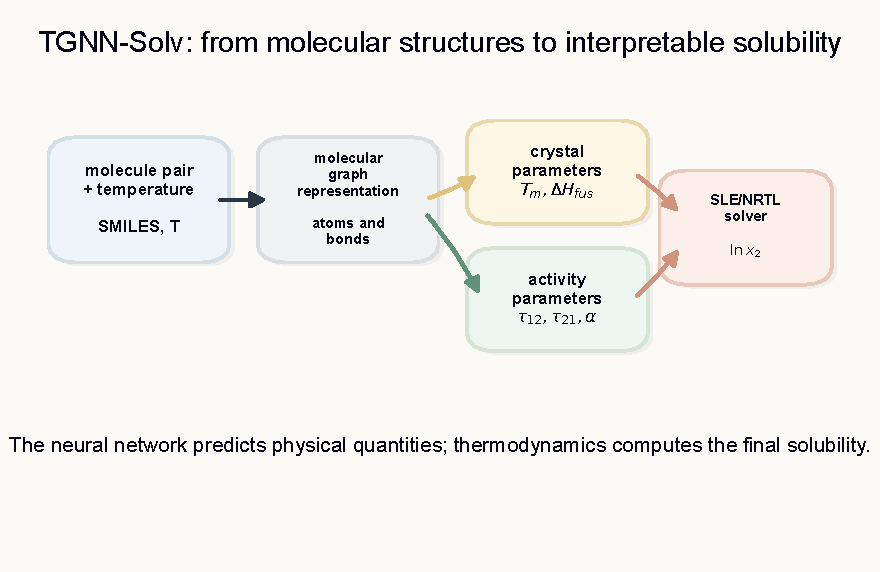
\includegraphics[width=0.94\textwidth]{graphical_abstract_schematic.pdf}
\caption{Общая логика TGNN-Solv: модель получает структуры вещества и растворителя, строит молекулярное представление, предсказывает физические параметры и передаёт их в термодинамический решатель.}
\label{fig:graphical-abstract}
\end{figure}

\newpage

\section{Ключевые термины и обозначения}
\label{sec:glossary}

В отчёте используются несколько устоявшихся сокращений. Ниже они собраны в одном месте, чтобы дальнейший текст можно было читать без обращения к программному коду.

\begin{table}[H]
\centering
\caption{Основные термины отчёта.}
\label{tab:glossary}
\begin{tabularx}{\textwidth}{P{0.23\textwidth}Y}
\toprule
Термин & Значение в этом отчёте \\
\midrule
Растворяемое вещество & Твёрдое органическое соединение, растворимость которого предсказывается; в формулах имеет индекс $2$. \\
Растворитель & Жидкая фаза, в которой растворяется вещество; в формулах имеет индекс $1$. \\
$\ln x_2$ & Целевая величина: натуральный логарифм мольной доли растворяемого вещества в насыщенном растворе. \\
Твёрдо-жидкое равновесие (SLE) & Условие равенства химических потенциалов вещества в твёрдой фазе и в насыщенном растворе. Именно из него получается основное уравнение модели. \\
Графовая нейронная сеть (GNN) & Модель, которая обрабатывает молекулу как граф: атомы являются узлами, химические связи --- рёбрами. \\
Молекулярный каркас & Остов молекулы по Мёрко: кольца и соединяющие их цепи без боковых заместителей. Разбиение по каркасам проверяет перенос на новые структурные классы. \\
TGNN-Solv & Разработанная в проекте модель: сначала предсказывает физические параметры, затем решает уравнение твёрдо-жидкого равновесия. \\
DirectGNN & Контрольная модель с тем же графовым представлением, но с прямым предсказанием $\ln x_2$ без физического уравнения. \\
NRTL & Термодинамическая модель коэффициентов активности в неидеальном растворе. В TGNN-Solv она задаёт вклад $\ln\gamma_2$. \\
IDAC & Коэффициент активности при бесконечном разбавлении. Такие данные не являются растворимостью; они дают частичный прямой сигнал на NRTL-ветвь, но одна IDAC-точка не определяет все параметры активности однозначно. \\
UNIFAC & Групповая модель активности растворов. В проекте она используется как источник физически осмысленных псевдометок и априорных оценок. \\
Групповой априорный прогноз & Оценка свойства по вкладам функциональных групп молекулы; в конфигурациях ей соответствуют параметры группы \code{use\_gc\_priors}. \\
Оракульная проверка & Диагностический режим, также называемый контрольным расчётом с известными параметрами: часть промежуточных физических параметров временно заменяется экспериментальными значениями, чтобы измерить вклад ошибки конкретного блока. \\
Плановый бюджет обучения & Базовая исследовательская схема обучения $50/200/50$ эпох по трём фазам. Короткие локальные запуски используются только как отладочные и диагностические. \\
\bottomrule
\end{tabularx}
\end{table}

\section{Постановка задачи}

Растворимость твёрдых органических веществ нужна не как абстрактная молекулярная характеристика, а как рабочий параметр химического эксперимента~\cite{bradley2014,boobier2017,vermeire2022,krasnov2025}. Она определяет выбор растворителя, температуру кристаллизации, выход очистки, риск выпадения осадка, пригодность формы вещества для разработки лекарственного препарата и границы технологического окна. Экспериментальное измерение при каждой новой паре вещество--растворитель и при каждой температуре дорого, поэтому надёжный расчётный прогноз имеет прямую практическую ценность.

Трудность состоит в том, что растворимость задаётся сразу двумя физическими объектами. Первый объект --- чистое твёрдое вещество: его температура плавления, энтальпия плавления, жёсткость, симметрия, склонность к плотной кристаллической упаковке. Второй объект --- жидкая смесь: совместимость функциональных групп растворяемого вещества и растворителя, водородные связи, полярность, дисперсионные взаимодействия, кислотно-основные эффекты и неидеальность раствора. Поэтому даже близкие по строению молекулы могут иметь разные растворимости, а одно и то же вещество может вести себя противоположно в воде, спирте и неполярном растворителе.

В работе рассматривается равновесная растворимость твёрдого органического вещества в жидком растворителе. На вход модели подаются:
\begin{enumerate}
    \item структура растворяемого вещества в формате SMILES;
    \item структура растворителя в формате SMILES;
    \item температура измерения $T$.
\end{enumerate}
На выходе требуется предсказать $\ln x_2$, где $x_2$ --- мольная доля растворяемого вещества в насыщенном растворе. Индекс $2$ используется для растворяемого вещества, индекс $1$ --- для растворителя.

Логарифм мольной доли выбран не только из численного удобства. Именно эта величина естественно появляется в уравнении твёрдо-жидкого равновесия, а логарифмическая шкала делает сопоставимыми хорошо растворимые и практически нерастворимые системы. Это важно: корпус содержит широкий диапазон растворимостей, и ошибка в линейной шкале была бы плохо связана с химической значимостью результата.

Цель проекта --- проверить, даёт ли явная термодинамическая структура преимущество перед прямым статистическим предсказанием. Физическая интерпретация здесь нужна по трём причинам. Во-первых, она позволяет отдельно смотреть на вклад кристалла и вклад раствора, а не получать один непрозрачный численный ответ. Во-вторых, она должна улучшать перенос по температуре, потому что форма зависимости от $T$ известна из термодинамики. В-третьих, она делает ошибки содержательными: можно понять, ошиблась ли модель в температуре плавления, энтальпии плавления или коэффициенте активности.

Поэтому поддерживается строгое сравнение двух моделей:
\begin{itemize}
    \item TGNN-Solv --- графовая модель с физическим слоем твёрдо-жидкого равновесия;
    \item DirectGNN --- такая же графовая обработка молекул, но прямое предсказание $\ln x_2$.
\end{itemize}
Если TGNN-Solv выигрывает, это должно происходить не из-за более сильного графового блока, а из-за физического ограничения. Если выигрывает DirectGNN, значит текущий физический путь вносит дополнительную ошибку или плохо идентифицирует промежуточные параметры.

\section{Данные}

\subsection{Состав корпуса}

Основной корпус построен на базе BigSolDB v2.1~\cite{krasnov2025,bigsoldb2026} и поддерживаемых в проекте обработанных таблиц \code{train.csv}, \code{val.csv}, \code{test.csv}. Важно различать два уровня данных. Полные обработанные таблицы содержат также строки со вспомогательными физическими метками; подмножество с метками растворимости содержит только строки, где используется целевая величина $\ln x_2$.

Текущий аудит обработанных таблиц даёт показатели из таблицы~\ref{tab:dataset}. Эти числа относятся к файлам, которые фактически используются текущими программами обучения и оценки.

\begin{table}[H]
\centering
\caption{Состав актуальных обработанных таблиц.}
\label{tab:dataset}
\begin{tabular}{lr}
\toprule
Показатель & Значение \\
\midrule
Все строки в обработанных таблицах & $127\,088$ \\
Строки с целевой растворимостью & $108\,287$ \\
Уникальные растворяемые вещества в строках растворимости & $1\,525$ \\
Уникальные растворители в строках растворимости & $212$ \\
Уникальные пары вещество--растворитель с метками растворимости & $12\,129$ \\
Диапазон температур в строках растворимости & $243.15$--$425.77\,\mathrm{K}$ \\
Средняя температура & $303.68\,\mathrm{K}$ \\
Медианная температура & $303.15\,\mathrm{K}$ \\
Среднее число строк на растворяемое вещество & $71.0$ \\
Медианное число строк на растворяемое вещество & $60$ \\
Среднее число температурных строк на пару & $8.93$ \\
Медианное число температурных строк на пару & $9$ \\
Полные дубликаты троек вещество--растворитель--температура & $0$ \\
Конфликтующие дубликаты таких троек & $0$ \\
\bottomrule
\end{tabular}
\end{table}

Отсутствие конфликтующих дубликатов важно для интерпретации ошибки: текущие значения MAE порядка $1.6$ нельзя объяснить тем, что в тесте часто встречаются одинаковые тройки с разными экспериментальными значениями. Главная сложность находится не в таких прямых противоречиях, а в переносе на новые вещества, новые каркасы и новые температурные области.

\begin{figure}[htbp]
\centering
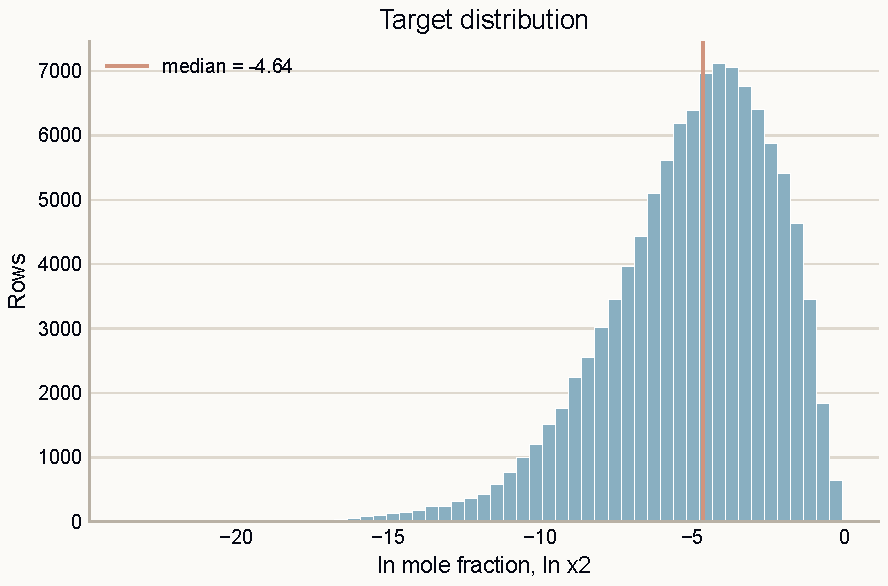
\includegraphics[width=0.66\textwidth]{corpus_lnx2_histogram.pdf}
\caption{Распределение целевой величины $\ln x_2$ в корпусе. Широкий диапазон растворимостей делает логарифмическую шкалу практически необходимой.}
\label{fig:corpus-lnx2}
\end{figure}

\begin{figure}[htbp]
\centering
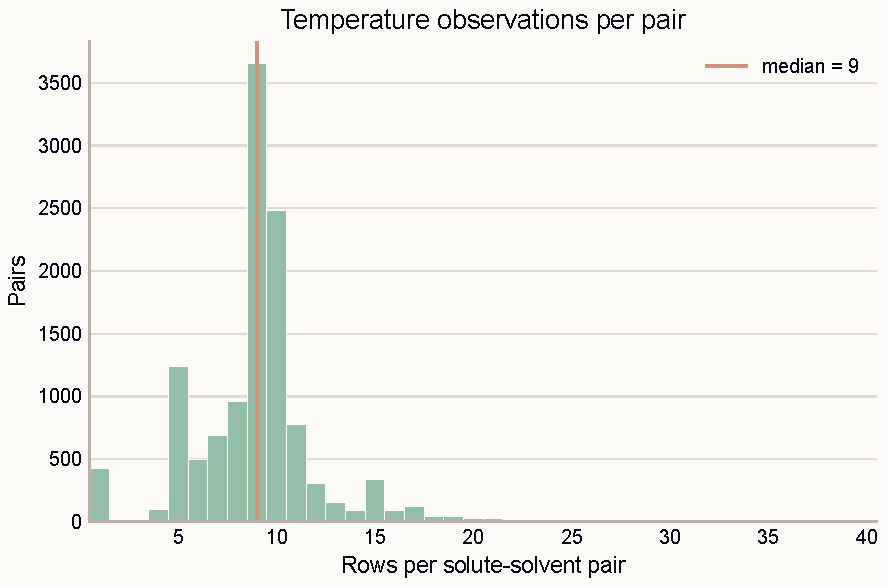
\includegraphics[width=0.66\textwidth]{corpus_points_per_pair.pdf}
\caption{Число температурных строк на пару вещество--растворитель. Наличие повторных температурных измерений позволяет проверять не только точечные прогнозы, но и форму температурных кривых.}
\label{fig:corpus-points-per-pair}
\end{figure}

\begin{figure}[htbp]
\centering
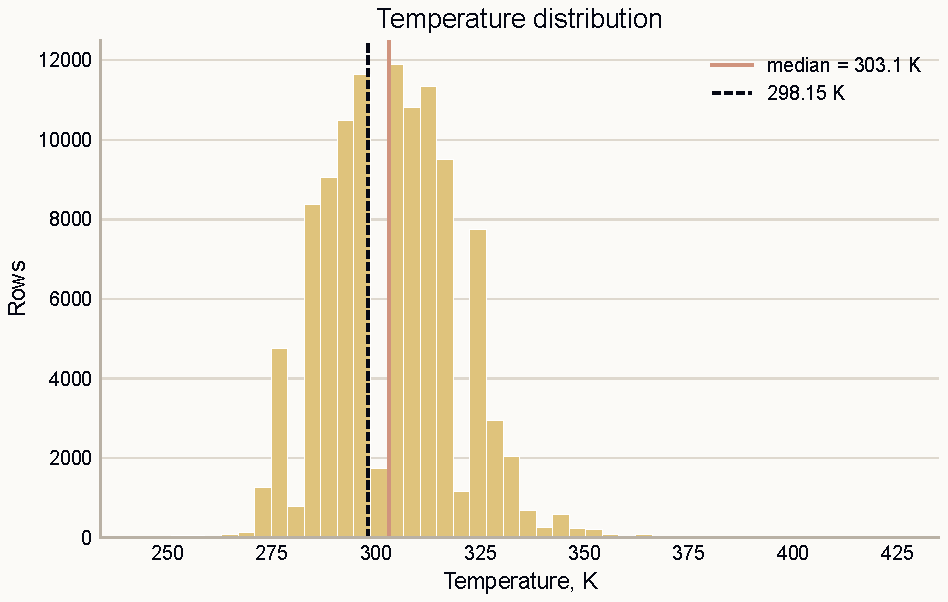
\includegraphics[width=0.66\textwidth]{corpus_temperature_histogram.pdf}
\caption{Распределение температур в строках растворимости. Основная масса измерений сосредоточена около комнатной температуры, поэтому перенос на высокие температуры проверяется отдельным протоколом, а не считается автоматически решённым общей метрикой.}
\label{fig:corpus-temperature}
\end{figure}

\begin{figure}[htbp]
\centering
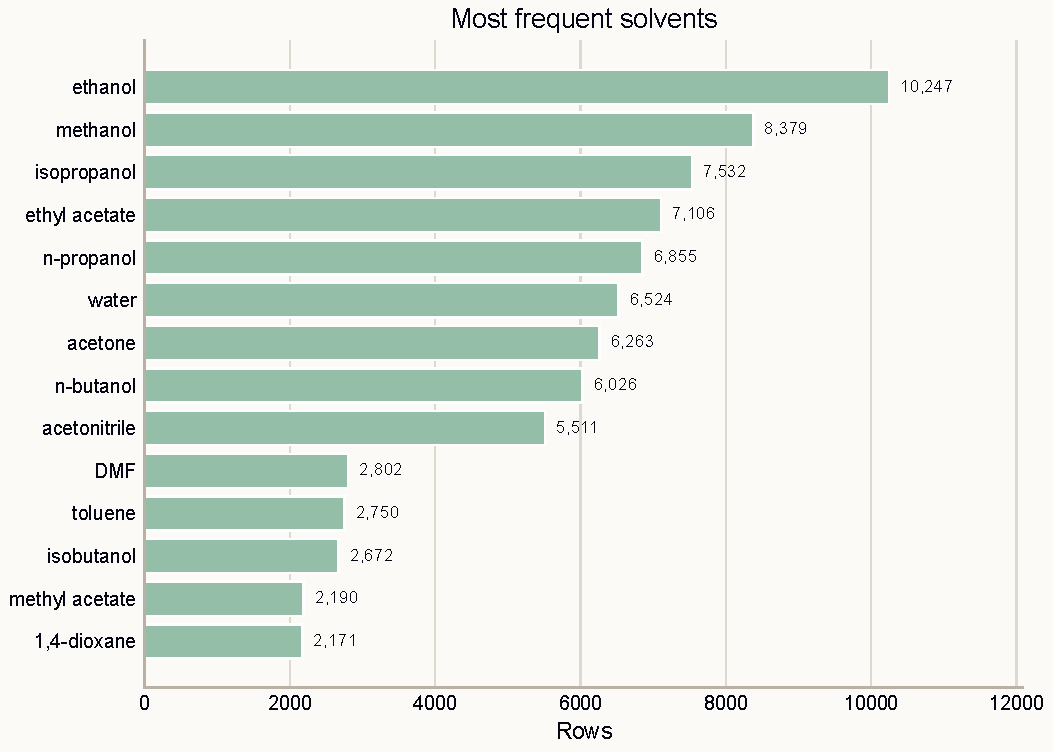
\includegraphics[width=0.72\textwidth]{corpus_solvent_barplot.pdf}
\caption{Наиболее частые растворители в корпусе. Распределение неравномерно: часть растворителей представлена тысячами строк, а длинный хвост растворителей встречается редко. Это важно для интерпретации ошибок на новых растворителях и водных системах.}
\label{fig:corpus-solvents}
\end{figure}

Эти распределения задают практическую геометрию задачи. Модель видит много повторных температурных рядов, но большинство из них лежит в узкой температурной области. Она также видит одни растворители существенно чаще других. Поэтому в отчёте отдельно разделяются три вопроса: перенос на новые структуры, перенос по температуре внутри той же пары и устойчивость к перекосу по источникам и растворителям.

Помимо целевой растворимости, в данных присутствуют или могут быть восстановлены вспомогательные физические величины: температура плавления $\Tm$, энтальпия плавления $\dHfus$, параметры Хансена, данные о коэффициенте активности при бесконечном разбавлении, групповые оценки кристаллических свойств, признаки растворителя и растворяемого вещества.

Покрытие вспомогательных величин неодинаково. В полных обработанных таблицах есть $73\,551$ строк с температурой плавления, но только $1\,279$ строк с прямой энтальпией плавления и $404$ строки с исходной IDAC-разметкой. Это создаёт асимметрию: кристаллическая часть модели получает гораздо более сильный прямой сигнал, чем часть, отвечающая за неидеальность раствора. Именно поэтому в проекте отдельно расширялся IDAC-корпус и добавлялись физические псевдометки.

\subsection{Как собирался основной корпус}

Сбор и приведение данных были отдельной частью работы, а не технической подготовкой перед моделированием. Главная таблица растворимости берётся из BigSolDB v2.1~\cite{krasnov2025,bigsoldb2026}. Затем записи приводятся к единому контракту: структуры растворяемого вещества и растворителя хранятся как канонические SMILES, температура --- в Кельвинах, целевая величина --- как $\ln x_2$. Строки, в которых растворимость доступна в другой шкале, переводятся в мольную долю; нечисловые, бесконечные и физически невозможные значения отбрасываются.

Второй принцип состоит в том, что растворимость и вспомогательные физические свойства не смешиваются в одну неразличимую таблицу. Для каждой строки есть маски: \code{has_solubility}, \code{has_T_m}, \code{has_dH_fus}, \code{has_hansen}, \code{has_gamma_inf}. Поэтому одна строка может участвовать в ошибке по растворимости, другая --- только в ошибке по температуре плавления, третья --- только в ошибке по коэффициенту активности. Это важно для честного обучения: отсутствующая метка не превращается в ноль и не создаёт ложный сигнал.

Дополнительно сохраняется происхождение строк. В проекте есть поля источника и диагностические программы, которые проверяют распределение измерений по источникам, возможные выбросы и дубликаты. Текущий аудит не нашёл конфликтующих полных дублей троек вещество--растворитель--температура. Тем самым дальнейшие ошибки модели нельзя списать на простое противоречие одинаковых экспериментальных записей.

\begin{figure}[H]
\centering
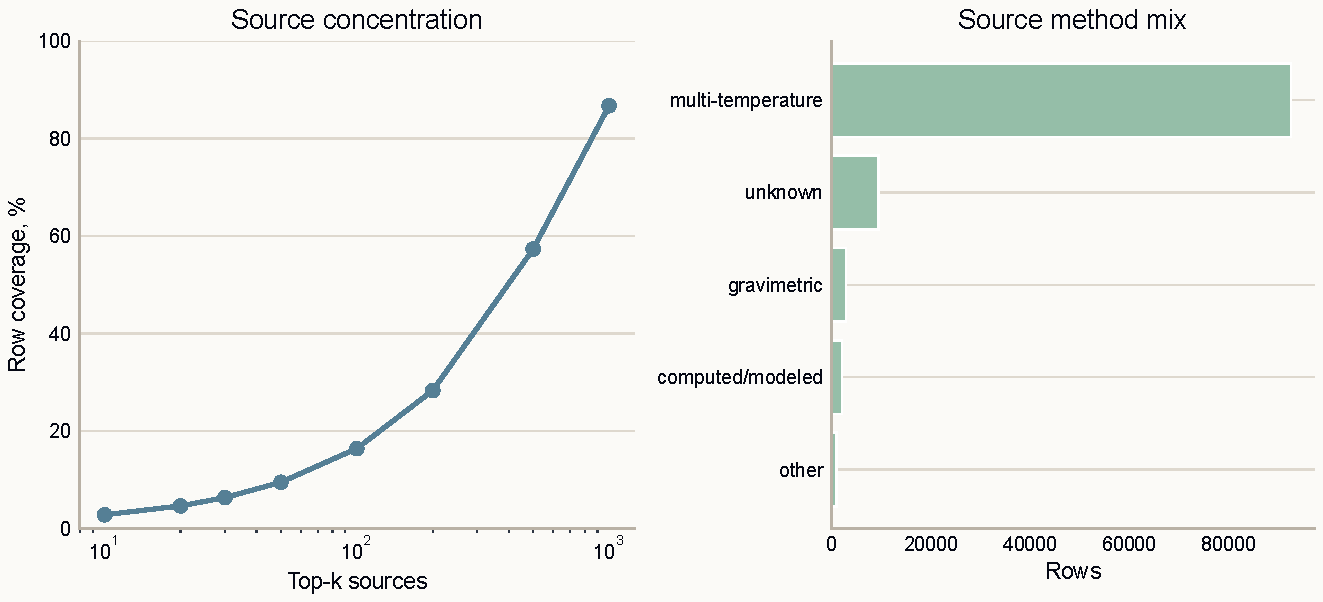
\includegraphics[width=0.92\textwidth]{source_uncertainty_coverage.pdf}
\caption{Аудит происхождения строк. Слева показано, какую долю корпуса покрывают наиболее крупные источники; справа --- приближённая смесь типов измерений после эвристической классификации. Такой аудит нужен, чтобы отделять физические ошибки модели от возможного перекоса корпуса по источникам.}
\label{fig:source-uncertainty-coverage}
\end{figure}

Отдельный результат этого аудита состоит в том, что корпус не сводится к нескольким доминирующим публикациям. Сто крупнейших источников дают около $16.4\%$ строк, пятьсот крупнейших --- около $57.3\%$. Низкая доля ста крупнейших источников связана с granularностью поля источника: в обработке многие записи различаются на уровне статьи, DOI или детализированного описания набора, а не только на уровне базы данных. Значит, источник данных может влиять на шум, но простое удаление одного-двух источников не решит задачу. По этой причине взвешивание источников было реализовано и проверено отдельно, а не принято как априорное улучшение.

\begin{figure}[H]
\centering
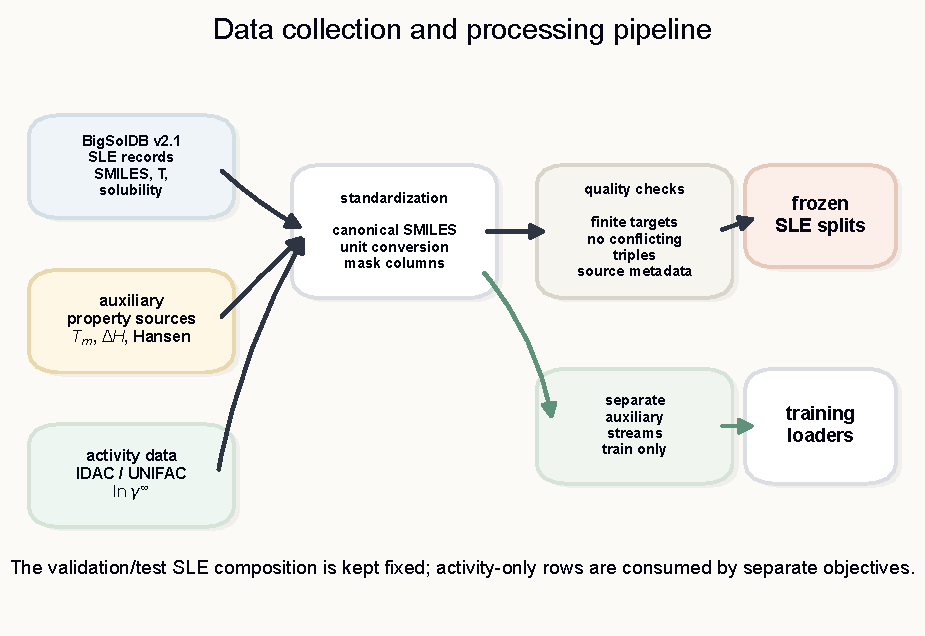
\includegraphics[width=0.96\textwidth]{data_collection_pipeline_schematic.pdf}
\caption{Схема подготовки данных. Основные SLE-строки фиксируют разбиения для оценки; вспомогательные физические данные подключаются через маски или отдельные обучающие потоки и не меняют состав валидационной и тестовой частей для растворимости.}
\label{fig:data-collection-pipeline}
\end{figure}

\subsection{IDAC-корпус для коэффициентов активности}

Особое внимание было уделено данным IDAC --- коэффициентам активности при бесконечном разбавлении. Причина проста: параметры NRTL почти не измеряются напрямую, а ошибка по растворимости видит только сумму кристаллического вклада и активности раствора. Поэтому без отдельного сигнала NRTL-ветвь может компенсировать ошибки кристаллической ветви, не становясь физически правильной.

Стартовый IDAC-набор был собран отдельно от BigSolDB как проверочный корпус для ветви активности. В файл \code{idac_seed_dois.txt} вошли $9$ вручную выбранных публикаций ThermoML; для них были загружены официальные NIST ThermoML JSON-записи, после чего тем же кодом извлечения были выбраны только бинарные жидкофазные измерения коэффициента активности при бесконечном разбавлении. В итоговом \code{idac.csv} сохранены DOI, номер набора в ThermoML, метод измерения, фаза, стандартное состояние, названия компонентов, InChI, RDKit-канонизированные SMILES, температура, $\gamma^\infty$ и $\ln\gamma^\infty$~\cite{idac_zenodo,frenkel2006,nist_thermoml}. Этот стартовый корпус содержит $404$ экспериментальные строки, $138$ пар и $9$ DOI; он достаточен для проверки схемы данных и обучения на малом примере, но слишком мал для устойчивой идентификации NRTL-параметров.

Поэтому был реализован расширенный извлекатель из NIST ThermoML~\cite{frenkel2006,nist_thermoml}. Он уже не ограничивается исходными DOI: программа проходит по DOI и страницам архива, кэширует ThermoML JSON, выбирает только бинарные IDAC-измерения, переводит стандартные InChI в SMILES с помощью RDKit, преобразует $\gamma^\infty$ в $\ln\gamma^\infty$ и сохраняет источник для каждой записи.

После извлечения выполняется очистка: удаляются нечисловые значения, отрицательные или нулевые $\gamma^\infty$, нераспознанные структуры и точные дубликаты. Затем строки агрегируются по ключу
\begin{equation*}
    (\mathrm{SMILES}_2,\mathrm{SMILES}_1,T),
\end{equation*}
где температура округляется до $10^{-3}\,\mathrm K$. Для обучения используется медианное значение $\ln\gamma^\infty$; параллельно сохраняются среднее, минимум, максимум, стандартное отклонение, число исходных записей и список DOI. Конфликтом считается группа со стандартным отклонением больше $0.5$ в $\ln\gamma^\infty$.

Итоговый расширенный IDAC-корпус содержит $14\,900$ агрегированных строк, $3\,145$ уникальных пар, $136$ растворяемых веществ, $112$ растворителей и $63$ DOI. Диапазон температур составляет $273.17$--$438.0\,\mathrm K$, диапазон $\ln\gamma^\infty$ --- от $-3.817$ до $8.178$. Конфликтующих агрегированных групп при пороге $0.5$ не обнаружено.

\begin{table}[H]
\centering
\caption{Расширение IDAC-данных.}
\label{tab:idac-corpus}
\begin{tabular}{lrr}
\toprule
Показатель & Стартовый набор & Расширенный набор \\
\midrule
Строки & $404$ & $14\,900$ \\
Уникальные пары & $138$ & $3\,145$ \\
Уникальные растворяемые вещества & --- & $136$ \\
Уникальные растворители & --- & $112$ \\
DOI-источники & $9$ & $63$ \\
Конфликтующие агрегированные группы & --- & $0$ \\
Точное пересечение с SLE-парами & --- & $0\%$ \\
Точное пересечение с SLE-тройками & --- & $0\%$ \\
\bottomrule
\end{tabular}
\end{table}

Отсутствие точного пересечения с SLE-парами имеет два следствия. Во-первых, расширенный IDAC-корпус не создаёт утечки целевой растворимости: он измеряет другую величину и на других парах. Во-вторых, он не может просто «подсказать» ответ для тестовых SLE-строк. Его роль другая: он обучает ту же функцию активности, которая затем используется в NRTL-слое для произвольной пары. Это одновременно является и ограничением: польза IDAC в SLE-задаче предполагает переносимость функции активности между химически разными парами. Поэтому окончательный вывод о вкладе IDAC требует абляции с одинаковым SLE-разбиением и включённым/выключенным вспомогательным IDAC-потоком; на текущем этапе такая полноразмерная абляция не завершена.

Поэтому IDAC не добавляется в SLE-таблицу как псевдорастворимость. В поддерживаемом протоколе он подаётся отдельным вспомогательным потоком: строки имеют \code{has_solubility=false}, \code{has_gamma_inf=true} и участвуют только в ошибке по $\ln\gamma^\infty$. Для контролируемых абляций также создана версия обработанных разбиений только для обучения: новые IDAC-строки добавляются только к обучающему файлу, а валидационная и тестовая части для растворимости остаются неизменными. В текущем потоке только для обучения используется $14\,876$ IDAC-строк и $3\,140$ пар; $404$ старых ключа уже присутствовали в исходной обработанной разметке и не дублируются.

UNIFAC-псевдометки имеют ещё более ограниченный статус. Они используются как слабый ориентир для $\ln\gamma^\infty$, но покрывают только часть текущего корпуса: в обработанном каркасном train-файле покрытие строк составляет $26.9\%$, в test-файле --- $8.6\%$, а покрытие уникальных пар в test --- $10.9\%$. Поэтому UNIFAC в отчёте не трактуется как самостоятельный сильный ориентир для новых каркасов. Нужны две отдельные проверки, которые ещё не закрыты: MAE UNIFAC на SLE-тесте там, где группы покрыты, и абляция TGNN-Solv с включёнными и выключенными UNIFAC-псевдометками при одинаковом SLE-разбиении.

\begin{figure}[H]
\centering
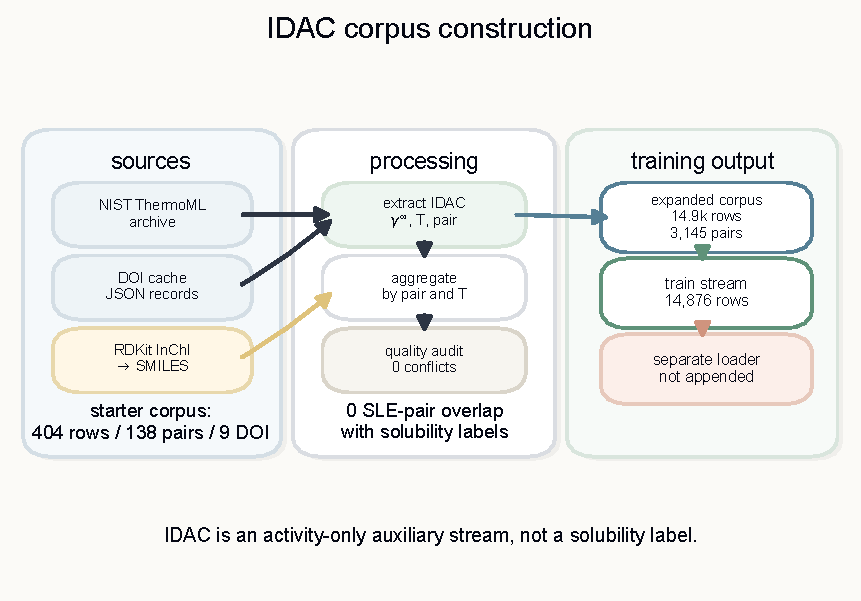
\includegraphics[width=0.96\textwidth]{idac_collection_pipeline_schematic.pdf}
\caption{Пайплайн сборки IDAC-корпуса. ThermoML используется как источник измерений активности, RDKit --- для стандартизации структур, а итоговый корпус подключается как отдельный обучающий сигнал для NRTL-ветви.}
\label{fig:idac-collection-pipeline}
\end{figure}

\begin{figure}[H]
\centering
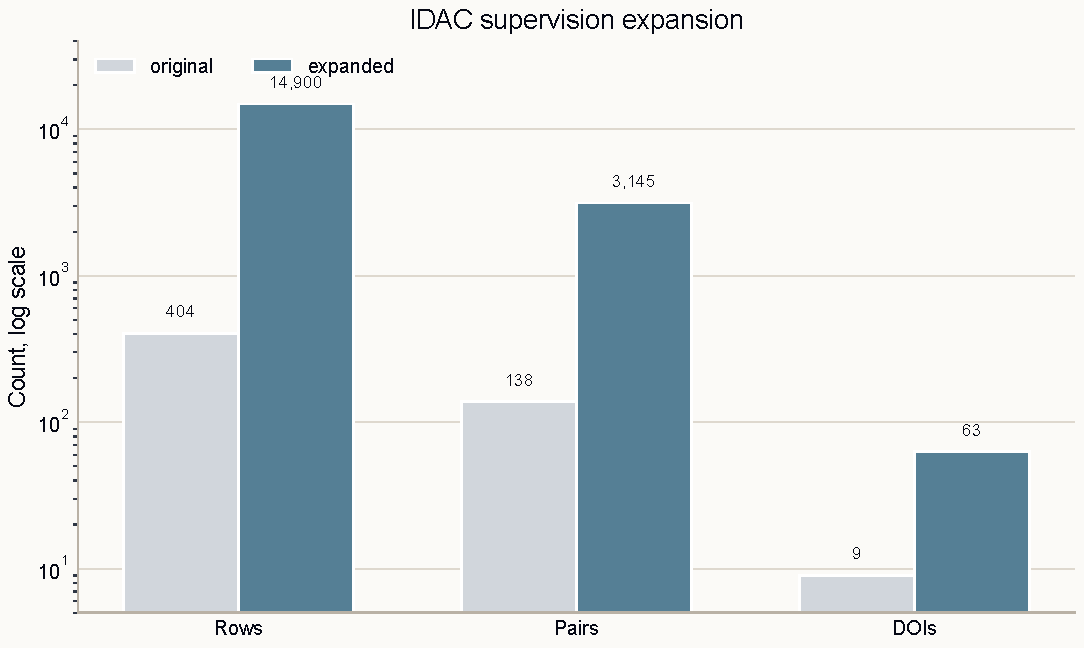
\includegraphics[width=0.76\textwidth]{idac_expansion_bars.pdf}
\caption{Масштаб расширения IDAC-разметки относительно стартового набора. Логарифмическая шкала используется только для совместного отображения строк, пар и DOI.}
\label{fig:idac-expansion}
\end{figure}

\subsection{Вода и малые растворители}

Вода сохранена в корпусе как обычный растворитель. В основном тесте по новым каркасам $476$ строк из $5\,826$ относятся к водным системам, то есть $8.17\%$. Малые растворители с числом тяжёлых атомов не больше трёх составляют $2\,104$ строки из $5\,826$, то есть $36.11\%$ теста.

Для графовой модели вода является особым случаем~\cite{landrum2024,gilmer2017}. При стандартном удалении водородов молекула $\mathrm{H_2O}$, записанная как SMILES \code{O}, превращается в граф из одного узла кислорода без обычных химических связей. Такой граф численно допустим, но беден: передача сообщений по связям почти не работает, а физические каналы, связанные с полярностью O--H, фактически не видят самих O--H связей.

Для этого реализован режим явных водородов для малых молекул. При его включении вода представляется как граф $\mathrm{H{-}O{-}H}$, то есть имеет три атома и направленные O--H связи. Размерность признаков не меняется, поэтому режим совместим с существующими моделями, но топология становится физически содержательнее.

\begin{figure}[H]
\centering
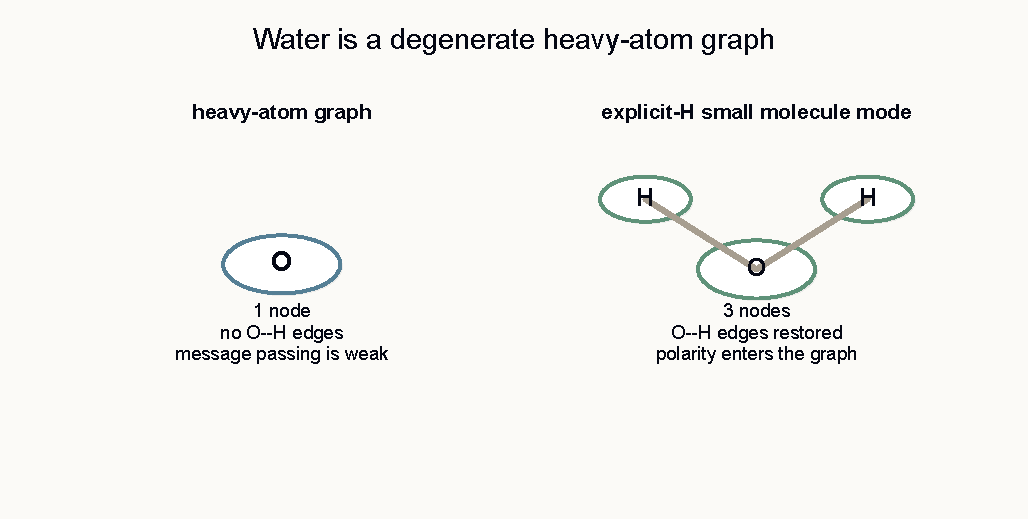
\includegraphics[width=0.88\textwidth]{water_graph_schematic.pdf}
\caption{Почему вода требует отдельного графового режима. В тяжелоатомном графе вода почти не даёт сообщения по связям; явные водороды возвращают O--H связи и делают полярную структуру доступной для графовой модели.}
\label{fig:water-graph}
\end{figure}

Текущие ошибки на водных строках близки у всех основных моделей: DirectGNN --- $2.199$, TGNN-Solv --- $2.203$, случайный лес --- $2.305$. Следовательно, вода сама по себе не объясняет отставание TGNN-Solv от DirectGNN, но её представление было исправлено как очевидный слабый случай графовой постановки.

\subsection{Разбиения данных}

В проекте используется несколько разбиений. Они нужны, чтобы разделить разные типы обобщения.

\begin{table}[H]
\centering
\caption{Основные режимы оценки.}
\begin{tabularx}{\textwidth}{lY}
\toprule
Разбиение & Что проверяет \\
\midrule
Случайные строки & Интерполяционный режим с сильным пересечением пар между обучением и тестом \\
Случайные пары & Новая пара, но оба компонента обычно уже встречались \\
Новый растворитель & Перенос на растворитель, отсутствующий в обучении \\
Новое вещество & Перенос на новый растворяемый компонент \\
Новый каркас & Перенос на новый структурный класс растворяемого вещества \\
Та же пара, новая температура & Физическую температурную зависимость внутри пары \\
\bottomrule
\end{tabularx}
\end{table}

Основное строгое разбиение для отчётности --- разбиение по молекулярным каркасам растворяемых веществ. Оно ближе к практической задаче, где требуется предсказывать свойства новых молекул, а не только новых температур для уже известных систем.

\begin{figure}[H]
\centering
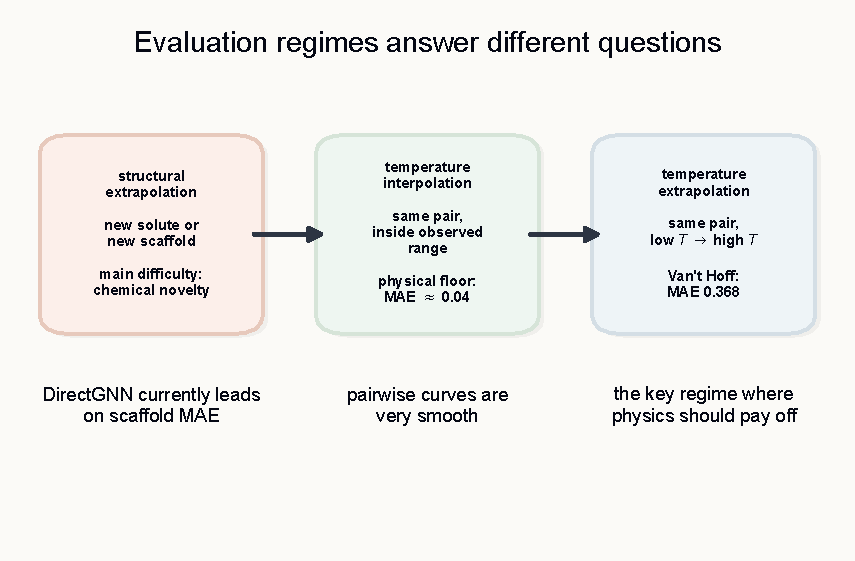
\includegraphics[width=0.92\textwidth]{evaluation_regimes_schematic.pdf}
\caption{Три принципиально разных режима оценки. Случайные строки проверяют почти интерполяцию; новые каркасы проверяют структурную экстраполяцию; температурные тесты для одной и той же пары проверяют, умеет ли модель использовать физическую форму зависимости от $T$.}
\label{fig:evaluation-regimes}
\end{figure}

\section{Обзор существующих подходов и внешних ориентиров}
\label{sec:methods-overview}

Существующие методы прогноза растворимости можно условно разделить на четыре группы~\cite{bradley2014,lusci2013,boobier2017,francoeur2021,vermeire2021,vermeire2022}. Они различаются не только точностью, но и тем, что именно считают: водную растворимость при одной температуре, растворимость в органических растворителях, коэффициенты активности или полное твёрдо-жидкое равновесие.

\begin{table}[H]
\centering
\caption{Основные классы методов, с которыми сопоставляется TGNN-Solv.}
\label{tab:method-overview}
\small
\begin{tabularx}{\textwidth}{P{0.20\textwidth}P{0.17\textwidth}Y P{0.20\textwidth}}
\toprule
Класс методов & Примеры & Что моделируют & Ограничение для текущей задачи \\
\midrule
Эмпирические и дескрипторные модели & GSE, QSPR, случайный лес & Прямую связь между молекулярными дескрипторами и растворимостью; часто хорошо работают как сильная практическая база & Обычно не разделяют вклад кристалла и раствора; температурная форма задаётся признаками, а не уравнением равновесия \\
Групповые термодинамические модели & UNIFAC, Modified UNIFAC & Коэффициенты активности через вклады функциональных групп~\cite{fredenslund1975,weidlich1987} & Требуют покрытия функциональных групп и не всегда хорошо работают для новых или сложных молекул \\
Модели избыточной энергии & NRTL, Wilson, UNIQUAC & Неидеальность жидкой смеси через параметры активности~\cite{renon1968,wilson1964,abrams1975} & Сами параметры нужно либо измерить, либо предсказать; без прямого обучающего сигнала они плохо идентифицируются \\
Графовые нейронные сети & MPNN, GAT, Chemprop-подобные модели & Структуру молекул как граф и прямое предсказание свойства~\cite{gilmer2017,velickovic2018,yang2019} & Обычно дают один итоговый скаляр и не гарантируют физически корректную температурную экстраполяцию \\
Внешние модели растворимости & SolProp, FastSolv & Современные прикладные ориентиры для растворимости в органических растворителях и воде~\cite{vermeire2022,fastsolv2025} & Обучаются и оцениваются в собственных протоколах; для честного сравнения в проекте они прогоняются через отдельные адаптеры \\
\bottomrule
\end{tabularx}
\end{table}

Отдельно полезно зафиксировать, какие модели неидеальности раствора были рассмотрены как физический слой. Они описывают одну и ту же термодинамическую величину --- избыточную энергию Гиббса или производные от неё коэффициенты активности, --- но имеют разные требования к данным.

\begin{table}[H]
\centering
\caption{Почему в основной версии выбран NRTL-слой, а альтернативы оставлены для абляций и приложений.}
\label{tab:activity-models}
\small
\begin{tabularx}{\textwidth}{P{0.16\textwidth}Y Y}
\toprule
Модель & Сильная сторона & Причина, по которой она не стала единственным основным вариантом \\
\midrule
NRTL & Работает с локальными составами, допускает асимметричные взаимодействия и естественно даёт $\gamma_i(x,T)$ для бинарной SLE-задачи~\cite{renon1968} & Параметры плохо идентифицируются без IDAC/VLE-подобного сигнала, поэтому их приходится супервизировать косвенно \\
Wilson & Численно гладкая и компактная форма для многих жидких смесей~\cite{wilson1964} & Менее удобна как универсальный слой для корпуса со сильной локальной неидеальностью и возможной ограниченной смешиваемостью; требует отдельной проверки области применимости, а не отвергается как физически неверная модель \\
UNIQUAC & Более явное разделение комбинаторного и остаточного вкладов~\cite{abrams1975} & Нужны дополнительные структурные параметры и аккуратная параметризация для большого набора органики \\
UNIFAC & Даёт переносимость через функциональные группы~\cite{fredenslund1975,weidlich1987} & Покрытие групп ограничивает новые молекулы; в проекте поэтому рассматривается как априорная оценка и источник псевдосигнала, а не как единственная модель \\
COSMO-RS & Физически богатая модель на основе поверхностных зарядов и квантово-химической информации~\cite{klamt1995} & Требует дорогого внешнего расчёта и не соответствует цели получить быстрый графовый предиктор для больших скринингов \\
\bottomrule
\end{tabularx}
\end{table}

Внутри проекта используются три типа базовых ориентиров. Первый --- случайный лес на молекулярных отпечатках и дескрипторах; он показывает, насколько далеко можно продвинуться без нейросетевого графового представления. Второй --- DirectGNN, то есть контрольная графовая модель с той же молекулярной частью, что и TGNN-Solv. Третий --- внешние программные модели SolProp и FastSolv, которые дают независимую точку отсчёта относительно современных прикладных решений.

Позиция TGNN-Solv между этими классами следующая. Модель использует гибкость графовых нейронных сетей, но не даёт им напрямую предсказывать растворимость. Вместо этого графовая часть оценивает физические параметры, а итоговое $\ln x_2$ получается из уравнения равновесия. Поэтому TGNN-Solv имеет более сложную задачу обучения, чем DirectGNN, но в случае успеха должна давать проверяемую декомпозицию ошибки и более устойчивый перенос по температуре.

\section{Термодинамическая основа модели}

\subsection{Уравнение равновесия}

В равновесии химический потенциал растворяемого вещества в твёрдой фазе равен химическому потенциалу того же вещества в жидком растворе~\cite{prausnitz1998,hildebrand1970}. Для жидкой фазы:
\begin{equation*}
    \mu_2^{\mathrm{liq}}(T,P,x)
    = \mu_2^{\mathrm{liq},0}(T,P) + RT\ln(\gamma_2 x_2).
\end{equation*}
Для чистого твёрдого вещества:
\begin{equation*}
    \mu_2^{\mathrm{sol}}(T,P)=\mu_2^{\mathrm{sol},0}(T,P).
\end{equation*}
Условие SLE даёт
\begin{equation*}
    \mu_2^{\mathrm{sol},0}(T)
    = \mu_2^{\mathrm{liq},0}(T) + RT\ln(\gamma_2 x_2).
\end{equation*}
Введём свободную энергию плавления:
\begin{equation*}
    \dGfus(T)=\mu_2^{\mathrm{liq},0}(T)-\mu_2^{\mathrm{sol},0}(T).
\end{equation*}
Тогда
\begin{equation*}
    \ln x_2 = -\frac{\dGfus(T)}{RT} - \ln\gamma_2.
\end{equation*}
Именно это уравнение является вычислительным ядром TGNN-Solv.

\begin{figure}[H]
\centering
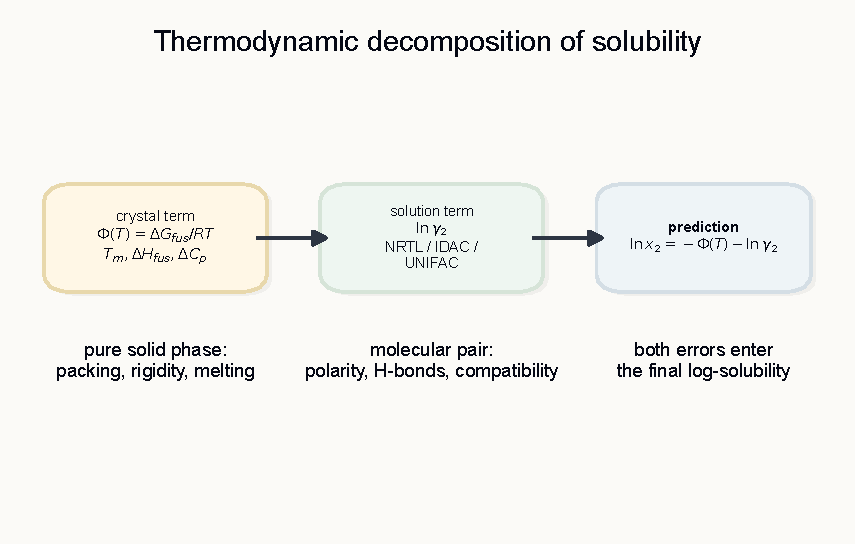
\includegraphics[width=0.90\textwidth]{sle_decomposition_schematic.pdf}
\caption{Физическое разложение $\ln x_2$ в TGNN-Solv. Кристаллическая часть задаёт стоимость плавления чистого вещества, а NRTL-часть описывает неидеальность жидкого раствора.}
\label{fig:sle-decomposition}
\end{figure}

\subsection{Кристаллический вклад}

В приближении нулевой теплоёмкостной поправки~\cite{hildebrand1970,yalkowsky1979}:
\begin{equation*}
    \Phi(T)=\frac{\dGfus(T)}{RT}
    =\frac{\dHfus}{R}\left(\frac{1}{T}-\frac{1}{\Tm}\right).
\end{equation*}
Если учитывать постоянную теплоёмкостную поправку, то
\begin{equation}
    \Phi(T)
    =\frac{\dHfus}{R}\left(\frac{1}{T}-\frac{1}{\Tm}\right)
    -\frac{\dCpfus}{R}\left(\frac{\Tm-T}{T}+\ln\frac{T}{\Tm}\right).
    \label{eq:phi-dcp}
\end{equation}
Вывод этой формулы приведён в приложении~\ref{app:fusion}. Он важен, потому что пренебрежение $\dCpfus$ может давать ошибку порядка $0.5$--$0.8$ в $\ln x_2$ для высокоплавких и сложных молекул. Это сравнимо с величиной улучшения, которую обычно ищут в моделях растворимости.

\begin{figure}[H]
\centering
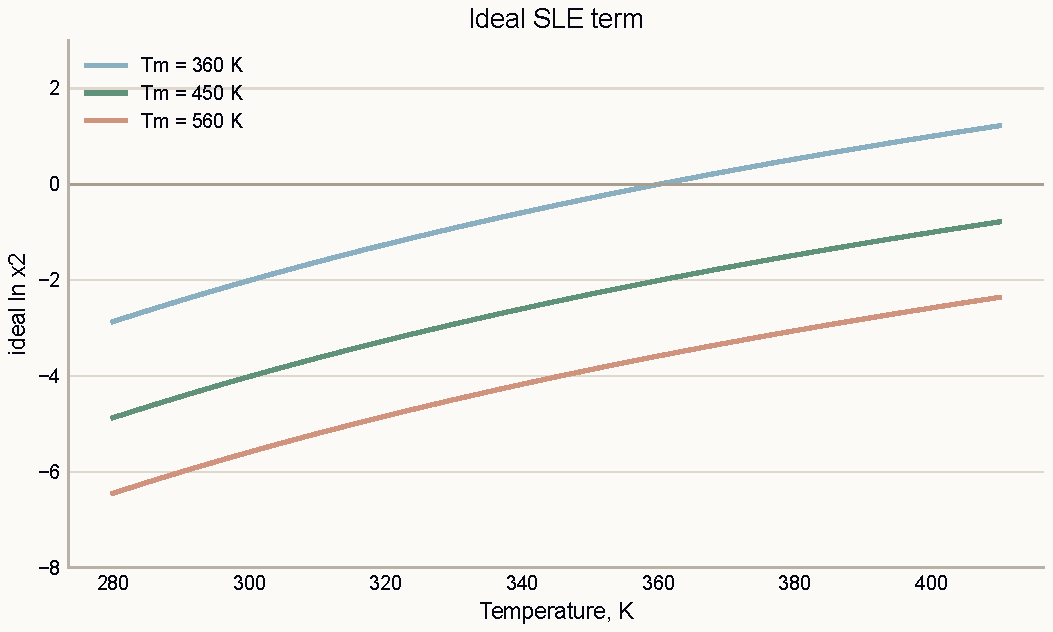
\includegraphics[width=0.82\textwidth]{ideal_sle_example.pdf}
\caption{Пример поведения идеальной части SLE: вклад плавления задаёт сильную температурную зависимость даже без учёта активности раствора.}
\label{fig:ideal-sle}
\end{figure}

Чувствительность этого члена достаточно велика, чтобы ошибки промежуточных параметров были заметны в итоговой растворимости. В приближении $\Delta C_p^{\mathrm{fus}}=0$:
\begin{equation*}
    \left|\delta \ln x_2\right|
    \approx
    \frac{\Delta H_{\mathrm{fus}}}{RT_m^2}\left|\delta T_m\right|.
\end{equation*}
Например, при $\Delta H_{\mathrm{fus}}=30\,\mathrm{kJ/mol}$, $T_m=450\,\mathrm K$ и ошибке $T_m$ на $30\,\mathrm K$ вклад в ошибку составляет примерно $0.53$ в $\ln x_2$. Это не малая величина относительно текущей разницы между TGNN-Solv и DirectGNN. Аналогично, ошибка энтальпии плавления на несколько $\mathrm{kJ/mol}$ может дать вклад порядка $0.5$--$0.7$ в $\ln x_2$. Поэтому физический путь требует не просто правильного уравнения, а достаточно точного предсказания промежуточных величин.

Теплоёмкостная поправка также не является заведомо малой. Для типичного порядка $T_m=500\,\mathrm K$, $T=298\,\mathrm K$ и $\Delta C_p^{\mathrm{fus}}=40\,\mathrm{J\,mol^{-1}K^{-1}}$ она даёт около $0.77$ в $\ln x_2$. Полная оценка вынесена в приложение~\ref{app:fusion}; в основном тексте важно только, что приближение $\Delta C_p^{\mathrm{fus}}=0$ может создавать систематическую ошибку масштаба, сравнимого с выигрышем сильных моделей.

\subsection{Активность раствора и NRTL}

Для коэффициента активности используется NRTL~\cite{renon1968,prausnitz1998}. В простейшей бинарной записи:
\begin{align*}
    G_{12} &= \exp(-\alpha\tau_{12}), \\
    G_{21} &= \exp(-\alpha\tau_{21}).
\end{align*}
Для растворённого вещества:
\begin{equation}
\ln\gamma_2
= x_1^2\left[
\tau_{12}\left(\frac{G_{12}}{x_2+x_1G_{12}}\right)^2
+ \frac{\tau_{21}G_{21}}{(x_1+x_2G_{21})^2}
\right].
\label{eq:nrtl}
\end{equation}
При бесконечном разбавлении $x_2\to0$, $x_1\to1$:
\begin{equation}
    \ln \gamma_2^{\infty}
    = \tau_{12}+\tau_{21}\exp(-\alpha\tau_{21}).
    \label{eq:idac}
\end{equation}
Эта формула связывает IDAC-данные с теми же параметрами активности, которые используются в SLE-решателе.

\begin{figure}[H]
\centering
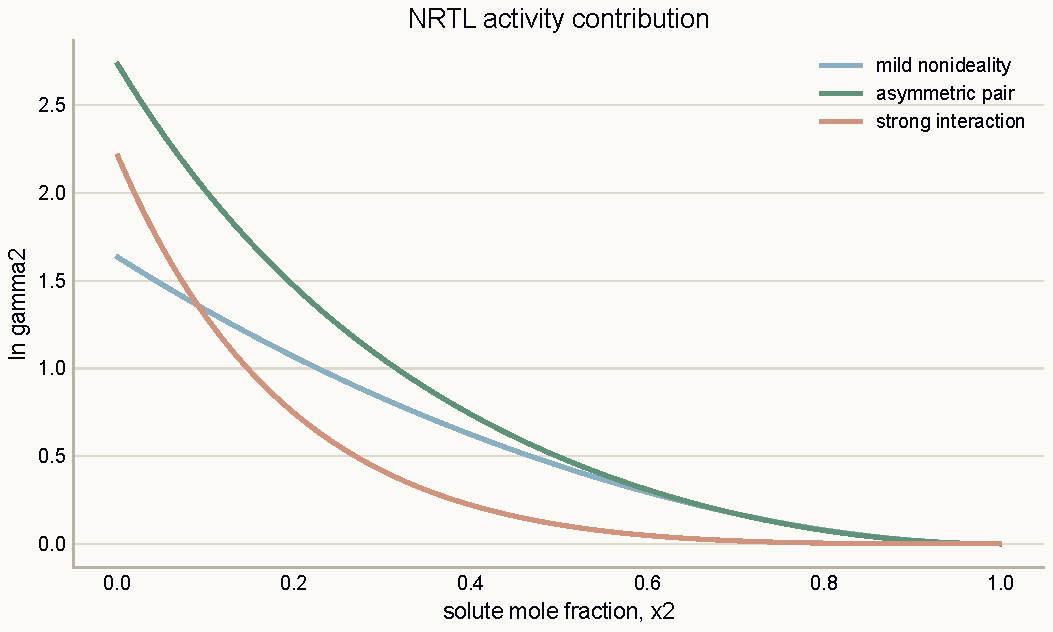
\includegraphics[width=0.82\textwidth]{nrtl_gamma_example.pdf}
\caption{Иллюстрация NRTL-вклада: изменение параметров $\tau_{12}$, $\tau_{21}$ и $\alpha$ меняет $\ln\gamma_2$ и тем самым сдвигает предсказанную растворимость.}
\label{fig:nrtl-gamma}
\end{figure}

\subsection{Почему задача плохо идентифицируема}

Из одного значения $\ln x_2$ невозможно однозначно восстановить все физические параметры; это типичный случай недоопределённой обратной задачи с физически осмысленными, но скрытыми параметрами~\cite{raissi2019,gould2021}. Разные комбинации $\Tm$, $\dHfus$, $\tau_{12}$, $\tau_{21}$ и $\alpha$ могут давать близкую растворимость. Даже несколько температур не всегда полностью снимают неоднозначность, потому что температурные вклады кристаллической части и активности частично коллинеарны. Формально это видно из линейной аппроксимации в приложении~\ref{app:identifiability}.

Следствие принципиально важно: хорошая итоговая ошибка по $\ln x_2$ не гарантирует физически правильные промежуточные параметры. Поэтому в проекте отдельно проверяются $\Tm$, $\dHfus$, $\tau_{12}$, $\tau_{21}$, $\Phi(T)$, $\ln\gamma_2$ и температурные наклоны.

\begin{figure}[H]
\centering
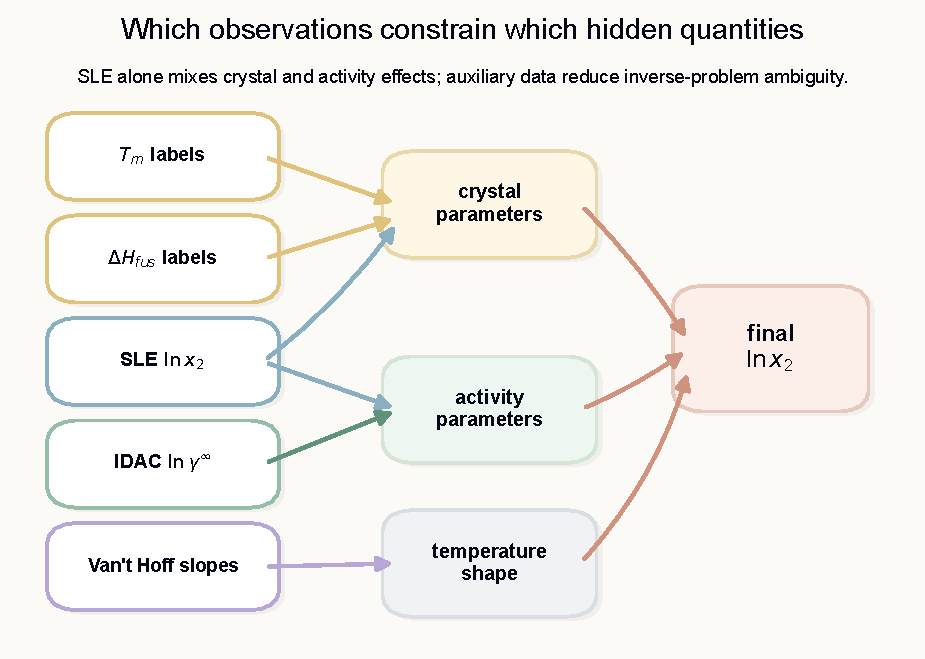
\includegraphics[width=0.94\textwidth]{identifiability_constraints_schematic.pdf}
\caption{Какие наблюдения ограничивают скрытые физические величины. Одна только SLE-метка смешивает кристаллический вклад и активность раствора; поэтому дополнительные данные нужны именно для идентифицируемости, а не для декоративного усложнения модели.}
\label{fig:identifiability-constraints}
\end{figure}

\begin{figure}[H]
\centering
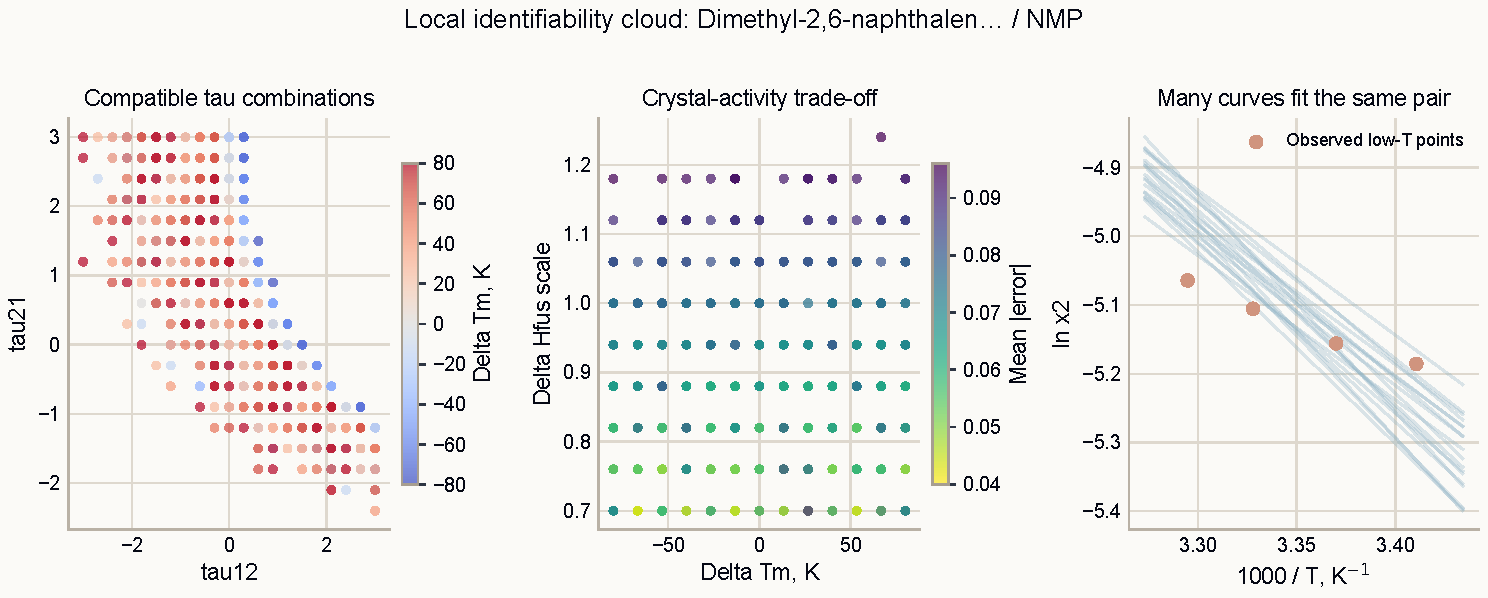
\includegraphics[width=0.96\textwidth]{degeneracy_visualization.pdf}
\caption{Локальная визуализация компенсаторной вырожденности на реальной температурной серии одной пары. Вокруг опорного решения существует заметное облако комбинаций $\Tm$, $\dHfus$, $\tau_{12}$ и $\tau_{21}$, которые воспроизводят те же низкотемпературные точки почти одинаково хорошо. Это не абстрактный довод, а наблюдаемая геометрия локальной обратной задачи.}
\label{fig:degeneracy-visualization}
\end{figure}

Рисунок~\ref{fig:degeneracy-visualization} добавляет важную интуицию к формальным выкладкам приложения. Даже если зафиксировать одну реальную пару и смотреть только на небольшой окрестности найденного решения, оказывается, что допустимых комбинаций параметров всё равно много. Поэтому слабая вспомогательная супервизия не обязана автоматически восстановить физически правильные $\tau_{12}$, $\tau_{21}$ или $\Tm$: она может оставить модель в области, где итоговая растворимость выглядит правдоподобно, но внутренние величины компенсируют друг друга.

\section{Архитектура TGNN-Solv и DirectGNN}

\subsection{Молекулярный граф и размер представления}

Молекулы представляются как графы: атомы являются узлами, химические связи --- рёбрами~\cite{gilmer2017,yang2019,landrum2024}. В базовой обработке один атом описывается не только атомным номером. В признаковый вектор входят валентность, степень, ароматичность, гибридизация, формальный заряд, число водородов, признаки донорно-акцепторного поведения, а также физико-химические подсказки вроде электроотрицательности, радиуса и поляризуемости. Базовый исторический формат корпуса имеет 35 атомных и 8 рёберных признаков; в TIMP-режиме к ним могут добавляться парциальный заряд Gasteiger и физические признаки связи.

Такое количество признаков не является избыточным украшением. Один атомный номер сообщает, что узел --- кислород, но не сообщает, находится ли он в гидроксильной группе, карбониле, эфире, ионизованной группе или воде. Для растворимости эти различия принципиальны: они меняют водородные связи, полярность, локальную доступность и вклад в коэффициент активности. Графовая сеть могла бы частично восстановить эти свойства из окружения, но тогда она тратила бы ёмкость и данные на изучение уже известных химических правил. Поэтому входные признаки задают химически осмысленную систему координат, а обучаемые слои решают более сложную задачу --- как эти признаки взаимодействуют в конкретной паре вещество--растворитель.

После нескольких слоёв передачи сообщений атомные состояния агрегируются в молекулярные векторы. Их размер больше числа исходных признаков, потому что это уже не таблица свойств атома, а скрытое представление роли молекулы в задаче: часть координат кодирует размер и форму, часть --- полярность и водородные связи, часть --- признаки, полезные для кристаллической ветви или для NRTL-параметров. Иными словами, высокая размерность нужна не для хранения атомного номера, а для одновременного описания нескольких физических аспектов молекулы.

\subsection{Агрегация атомных состояний в вектор молекулы}

После передачи сообщений модель всё ещё имеет набор атомных состояний $\{h_i\}$, а физическим выходным блокам нужен один вектор молекулы. Поэтому используется не простое усреднение, а многоканальная агрегация. Она объединяет два механизма:
\begin{equation*}
    g_{\mathrm{attn}}
    =
    \sum_{i\in G} a_i h_i,
    \qquad
    a_i=
    \frac{\exp u(h_i)}{\sum_{j\in G}\exp u(h_j)},
\end{equation*}
и Set2Set-агрегацию:
\begin{equation*}
    g_{\mathrm{s2s}}=\operatorname{Set2Set}(\{h_i:i\in G\}).
\end{equation*}
Итоговый вектор равен
\begin{equation*}
    g_{\mathrm{mol}}=[g_{\mathrm{attn}},g_{\mathrm{s2s}}],
\end{equation*}
поэтому его размерность равна $3d$ при скрытой размерности атомного состояния $d$. Часть с вниманием позволяет модели выделять функциональные группы, которые важны для конкретного свойства, а Set2Set сохраняет более глобальную информацию о форме и составе молекулы. В TIMP-режиме к этому добавляются отдельные агрегации дисперсионного и полярного каналов:
\begin{equation*}
    g_{\mathrm{mol}}^{\mathrm{TIMP}}
    =
    [g_{\mathrm{attn}},g_{\mathrm{s2s}},g_{\mathrm{disp}},g_{\mathrm{polar}}].
\end{equation*}
Это объясняет, почему агрегация атомных состояний является самостоятельной частью архитектуры, а не техническим средним по атомам: именно здесь локальные атомные сообщения превращаются в физически пригодные молекулярные координаты.

\begin{figure}[H]
\centering
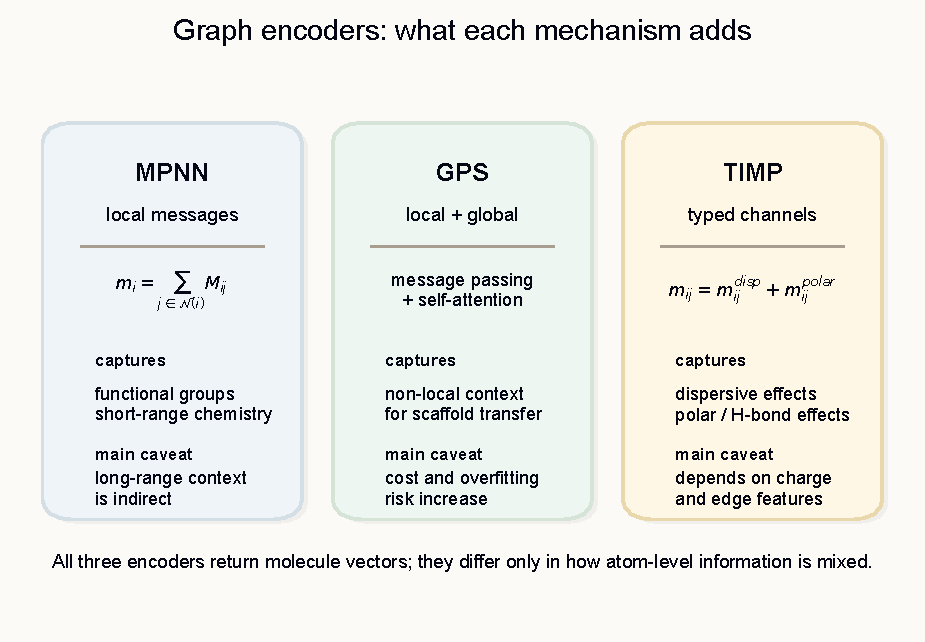
\includegraphics[width=0.96\textwidth]{graph_mechanisms_schematic.pdf}
\caption{Три поддерживаемых механизма графового кодирования. MPNN использует локальную передачу сообщений; GPS добавляет глобальное внимание; TIMP разделяет сообщения на дисперсионный и полярно-ассоциативный каналы.}
\label{fig:graph-mechanisms}
\end{figure}

\subsection{Передача сообщений, GPS и TIMP}

Базовый MPNN обновляет состояние атома через сообщения от соседей:
\begin{equation*}
    m_i^{(\ell)}=\sum_{j\in\mathcal N(i)}
    M_\ell(h_i^{(\ell)},h_j^{(\ell)},e_{ij}),
    \qquad
    h_i^{(\ell+1)}=U_\ell(h_i^{(\ell)},m_i^{(\ell)}).
\end{equation*}
Такой блок хорошо описывает локальные химические окружения. Его слабость --- дальние связи в молекуле и глобальные эффекты формы: сигнал между удалёнными фрагментами проходит через несколько слоёв и может затухать. Поэтому реализован вариант GPS/GraphGPS: локальная передача сообщений дополняется глобальным самовниманием по атомам графа и позиционными кодировками~\cite{rampasek2022,vaswani2017}. Этот вариант проверяет, помогает ли глобальный контекст при переносе на новые каркасы.

TIMP был добавлен как более физически направленное исправление. В обычном MPNN все связи обрабатываются одним типом сообщения. В TIMP сообщение раскладывается на два канала:
\begin{equation*}
    m_{ij}
    =
    m_{ij}^{\mathrm{disp}}
    +
    m_{ij}^{\mathrm{polar}},
\end{equation*}
где дисперсионный канал масштабируется признаками поляризуемости, а полярный канал --- парциальными зарядами, разностью электроотрицательностей и способностью к водородной связи. Это не квантово-химический расчёт энергии, а физически осмысленная декомпозиция обучаемых сообщений. Её смысл в том, что параметры NRTL описывают эффективные энергии контактов, поэтому на вход NRTL-блока лучше подавать не один «серый» вектор, а представление, где дисперсионные и полярные эффекты уже частично разведены.

\begin{figure}[H]
\centering
\includegraphics[width=0.92\textwidth]{timp_hansen_diagnostics.pdf}
\caption{Диагностика TIMP и контрастивное выравнивание по параметрам Хансена. По линейной пробе TIMP с контрастивным выравниванием повышает медианный $R^2$ восстановления RDKit-дескрипторов, а каналовая диагностика показывает почти ортогональные дисперсионный и полярный каналы. Это диагностика представления, а не доказанный выигрыш итогового MAE.}
\label{fig:timp-hansen-diagnostics}
\end{figure}

Контрастивное выравнивание по параметрам Хансена следует понимать как метрическое обучение, а не как строгое доказательство физической интерпретируемости канала. Если два вещества близки по $\delta_d$ или $\delta_p$, штраф сближает соответствующие представления, но сеть всё ещё может использовать коррелирующие признаки, например молярный объём, ароматичность или число гетероатомов. Поэтому TIMP-диагностика показывает доступность физико-химических координат в представлении, а не гарантирует, что конкретная координата является чистой дисперсионной или полярной энергией.

\subsection{Представление пары и перекрёстное внимание}

Графовый блок получает два графа: растворяемого вещества и растворителя. Затем строится представление пары. Базовый вариант использует перекрёстное внимание~\cite{vaswani2017}: атомы одной молекулы формируют запросы, атомы другой --- ключи и значения. Так модель получает мягкую карту потенциальных контактов между функциональными группами двух компонентов. После агрегации строится парный вектор
\begin{equation*}
    g_{\mathrm{pair}}
    =
    [g_2,\;g_1,\;g_2\odot g_1,\;|g_2-g_1|],
\end{equation*}
а в режимах с дескрипторным дополнением к нему добавляется аналогичный блок из нормированных RDKit-дескрипторов. Это важно: дескрипторы не обходят физический слой, а обогащают вход для физических выходных блоков.

В этой части обнаружено важное слабое место. Кристаллические выходные блоки получают много прямых меток $\Tm$, тогда как NRTL-параметры почти не размечены напрямую. Поэтому градиент к парному взаимодействию идёт в основном через SLE-решатель и может быть слабым или плохо обусловленным. Для борьбы с этим реализованы три механизма: отдельный IDAC-поток для активности, вспомогательная прямая ошибка по растворимости на парном векторе только во время обучения и частичное ослабление кристаллического градиента во второй фазе. Эти механизмы не меняют физический расчёт при применении модели, а должны «оживить» представление пары.

\begin{figure}[H]
\centering
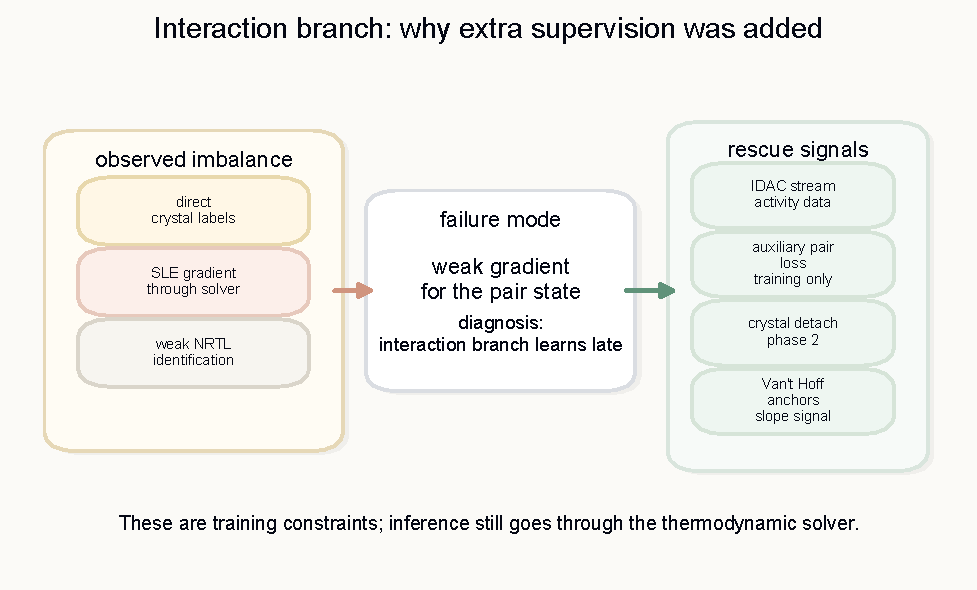
\includegraphics[width=0.94\textwidth]{interaction_rescue_schematic.pdf}
\caption{Перекрёстное внимание строит признаки контакта между молекулами, но его обучение может голодать по градиенту, потому что основной путь к NRTL идёт через решатель. В проекте реализованы прямой вспомогательный сигнал на парный вектор, IDAC-якоря и режимы ослабления кристаллического градиента.}
\label{fig:interaction-rescue}
\end{figure}

\subsection{Физический путь TGNN-Solv}

TGNN-Solv состоит из следующих логических частей:
\begin{enumerate}
    \item графовая обработка растворяемого вещества и растворителя;
    \item построение парного представления, при необходимости с маршрутизацией по типу растворителя;
    \item блок кристаллических свойств, оценивающий $\Tm$, $\dHfus$ и в некоторых режимах $\dSfus$ или $\dCpfus$;
    \item блок взаимодействия пары, оценивающий параметры активности NRTL;
    \item численный решатель уравнения SLE;
    \item ограниченная поправка в пространстве физических параметров.
\end{enumerate}

\begin{figure}[H]
\centering
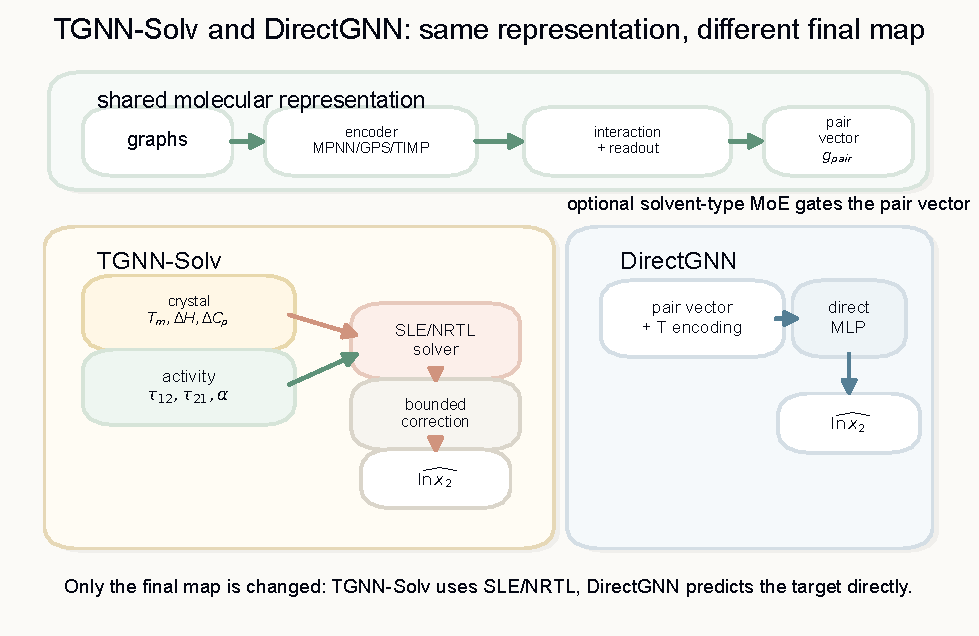
\includegraphics[width=0.96\textwidth]{architecture_schematic.pdf}
\caption{Схема двух поддерживаемых моделей. DirectGNN нужен как строгий контроль: графовый блок тот же, отличие состоит в наличии или отсутствии физического SLE-слоя.}
\label{fig:architecture}
\end{figure}

Маршрутизация по типу растворителя реализована как смесь экспертов. Пусть $c$ --- дискретный тип растворителя, а $e(c)$ --- его обучаемое векторное представление. Тогда сеть маршрутизации строит веса экспертов
\begin{equation*}
    \pi_k
    =
    \operatorname{softmax}_k
    W_g[g_{\mathrm{pair}},e(c)],
\end{equation*}
а сами эксперты дают преобразования $E_k(g_{\mathrm{pair}})$. Обновление имеет остаточный вид:
\begin{equation*}
    g_{\mathrm{pair}}'
    =
    g_{\mathrm{pair}}
    +
    \tanh\rho
    \sum_k \pi_k E_k(g_{\mathrm{pair}}).
\end{equation*}
Параметр $\rho$ инициализируется так, чтобы в начале блок почти не менял представление. Это сделано намеренно: водные, спиртовые, ароматические и неполярные растворители имеют разные типичные механизмы неидеальности, но смесь экспертов не должна сразу разрушать базовый парный вектор. Для контроля добавлен слабый штраф на баланс экспертов, чтобы все примеры не ушли в один и тот же эксперт.

Важно не переоценивать этот блок. Смесь экспертов по типам растворителей реализована и доступна в конфигурации, но её изолированный вклад в итоговый MAE ещё не доказан полноразмерной абляцией. Поэтому в этом отчёте она трактуется как подготовленная архитектурная возможность, а не как установленная причина улучшения качества.

Итоговый ответ TGNN-Solv получается не из отдельной регрессионной формулы, а из вычисления $\Phi(T)$, $\ln\gamma_2$ и решения SLE. Поэтому у результата есть проверяемая внутренняя структура: можно отдельно анализировать вклад кристалла, вклад активности раствора и остаточную поправку. Если итоговая ошибка велика, диагностика может показать, где именно она возникает.

Важное расширение --- энтропийно согласованная кристаллическая параметризация~\cite{yalkowsky1979,acree2010}. Вместо независимого предсказания $\Tm$ и $\dHfus$ модель может предсказывать $\dHfus$ и $\dSfus$, а затем вычислять
\begin{equation*}
    \Tm = \frac{\dHfus}{\dSfus}.
\end{equation*}
Такое представление лучше согласовано с термодинамикой и позволяет вводить мягкое ограничение на энтропию плавления.

\subsection{Температура и остаточная физическая коррекция}

Температура кодируется в двух моделях по-разному. В TGNN-Solv она входит в физические формулы через $1/T$, $\Phi(T)$ и температурную форму NRTL-параметров. В DirectGNN используется обучаемое температурное кодирование, похожее на набор мягких индикаторов температурных интервалов, после чего температура поступает в прямой выходной блок. Поэтому температурные тесты отвечают не только на вопрос качества, но и на вопрос формы: кто лучше восстанавливает наклон $\ln x_2$ как функции $1/T$.

\begin{figure}[H]
\centering
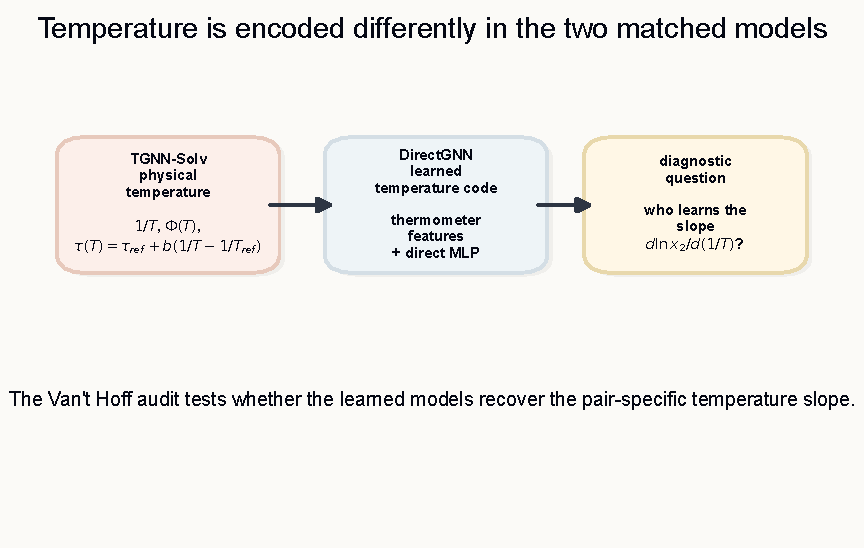
\includegraphics[width=0.88\textwidth]{temperature_encoding_schematic.pdf}
\caption{Кодирование температуры в TGNN-Solv и DirectGNN. В физической модели температура входит в SLE и NRTL явно; в прямой модели она передаётся как обучаемые температурные признаки.}
\label{fig:temperature-encoding}
\end{figure}

Остаточная коррекция в TGNN-Solv тоже устроена физически. Она не добавляет свободный нейросетевой сдвиг к $\ln x_2$. Сначала базовые параметры проходят через SLE-решатель. Затем отдельный блок предлагает ограниченные поправки к $\Tm$, $\dHfus$, $\tau_{12}$ и $\tau_{21}$, после чего SLE решается повторно. Итог смешивается с базовым решением через ограниченный gate. Поэтому даже коррекция остаётся диагностируемой: можно измерить, какие физические параметры она меняет и насколько.

\begin{figure}[H]
\centering
\includegraphics[width=0.90\textwidth]{correction_loop_schematic.pdf}
\caption{Остаточная коррекция TGNN-Solv работает в пространстве физических параметров и требует повторного решения SLE. Это сохраняет интерпретируемость и ограничивает превращение модели в прямую регрессию.}
\label{fig:correction-loop}
\end{figure}

\subsection{DirectGNN как контроль}

DirectGNN использует тот же графовый блок и тот же способ построения парного представления, что и TGNN-Solv, но вместо физической ветви имеет прямой регрессионный выход на $\ln x_2$.

Это не просто ещё одна конкурирующая модель, а контрольный эксперимент. У DirectGNN и TGNN-Solv совпадают молекулярный графовый блок, способ построения представления пары, целевая величина и разбиения данных. Различается только финальный путь: DirectGNN сразу предсказывает $\ln x_2$, а TGNN-Solv проходит через физические параметры и решатель.

Такое сравнение изолирует цену физического узкого места. Если DirectGNN выигрывает, это не доказывает, что молекулярные графы бесполезны или что данные не моделируются. Это означает более конкретную вещь: текущий физический путь либо усиливает ошибки промежуточных параметров, либо недостаточно хорошо идентифицирует параметры кристалла и активности.

\subsection{Вспомогательные сигналы}

В модель и обучение добавлены:
\begin{itemize}
    \item прямые метки $\Tm$ и $\dHfus$;
    \item параметры Хансена и их парные разности~\cite{hansen2007};
    \item IDAC-данные для $\ln\gamma_2^\infty$~\cite{frenkel2006,nist_thermoml};
    \item групповые оценки кристаллических свойств~\cite{joback1987,marrero2001};
    \item оценки UNIFAC для части пар~\cite{fredenslund1975,weidlich1987};
    \item температурные ограничения по кривым Вант-Гоффа;
    \item явные водороды для малых молекул;
    \item режимы ослабления конфликта между кристаллической и парной частями.
\end{itemize}
Не все эти расширения уже доказали улучшение качества. Часть из них является подготовленной инфраструктурой для следующей серии проверок. В основных таблицах учитываются только проведённые воспроизводимые сравнения.


\section{Обучение, функция ошибки и протокол оценки}
\label{sec:training}

Физически-информированную модель нельзя устойчиво обучать как обычную регрессию «граф $\rightarrow$ число». Если в начале обучения случайные параметры сразу попадают в SLE-решатель, то модель получает плохо обусловленные градиенты: кристаллическая часть, активность раствора и остаточная поправка начинают компенсировать ошибки друг друга. Поэтому обучение построено как последовательность режимов с возрастающей сложностью.

\subsection{Этап 0: предобучение графового блока}
\label{sec:stage0-pretraining}

До основной регрессии растворимости поддержан этап 0 --- предобучение графового блока на молекулярных задачах, которые не требуют измеренной растворимости. Его смысл не в том, чтобы сразу научить модель термодинамике растворов, а в том, чтобы дать графовому блоку химически осмысленную инициализацию: валентность, типы связей, ароматические окружения, полярность, размер и общие дескрипторные свойства молекул.

В текущем контуре реализованы четыре класса задач предобучения:
\begin{enumerate}
    \item восстановление маскированных атомных признаков по окружению;
    \item предсказание типа химической связи;
    \item восстановление набора RDKit-дескрипторов из молекулярного представления;
    \item контрастивное сближение двух слегка искажённых представлений одной молекулы и разведение разных молекул.
\end{enumerate}
После этапа 0 временные выходные блоки удаляются, а веса графового блока используются как тёплый старт для TGNN-Solv и DirectGNN. Это важно методически: если предобучение применяется только к одной модели, сравнение физического и прямого путей становится нечестным.

\begin{figure}[H]
\centering
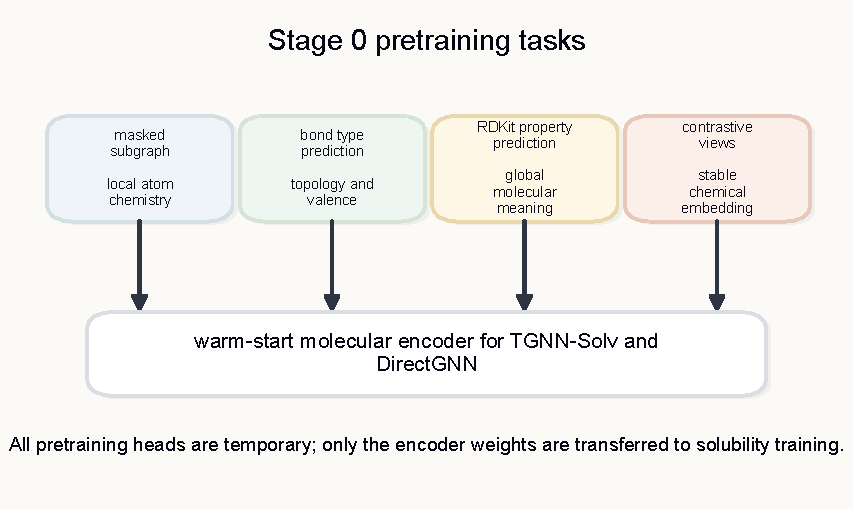
\includegraphics[width=0.92\textwidth]{pretraining_tasks_schematic.pdf}
\caption{Этап 0: вспомогательные задачи предобучения графового блока. Они улучшают молекулярное представление, но сами по себе ещё не учат термодинамическую совместимость пары вещество--растворитель.}
\label{fig:pretraining-tasks}
\end{figure}

Важное ограничение этого этапа уже зафиксировано в проектной памяти и диагностике: предобучение на одиночных молекулах не заменяет парную информацию. Оно может улучшить представление тиофенового кольца или карбонильной группы, но не сообщает напрямую, как данное вещество взаимодействует с водой, этанолом или гексаном. Поэтому для следующего этапа подготовлены парные задачи предобучения: близость растворимостей в одном растворителе, трудные отрицательные примеры с близкой структурой и разной растворимостью, а также предсказание разностей параметров Хансена.

Отдельно реализована диагностика качества представлений после таких блоков. На замороженных векторных представлениях обучается простая линейная модель, которая пытается восстановить стандартные химические дескрипторы. Эта проверка нужна потому, что низкий MAE сам по себе не говорит, что графовый блок действительно содержит LogP, полярную поверхность, число доноров и акцепторов водородной связи. В старых промежуточных проверках медианный $R^2$ такой линейной пробы был около $0.505$, то есть базовый MPNN сохранял только часть информации, которую сильная дескрипторная модель получает явно. После добавления TIMP и контрастивного выравнивания по параметрам Хансена медианный показатель в диагностическом срезе вырос до $0.601$, а число хорошо восстанавливаемых дескрипторов увеличилось. Это не финальный результат по растворимости, но это важное объяснение, почему работа над представлением не менее важна, чем работа над решателем.

\subsection{Три фазы основного обучения}

Основное обучение TGNN-Solv проводится в три фазы. Канонический плановый бюджет --- $50/200/50$ эпох: 50 эпох физического разогрева, 200 эпох SLE-обучения и 50 эпох тонкой настройки с меньшим шагом оптимизации.

\begin{figure}[H]
\centering
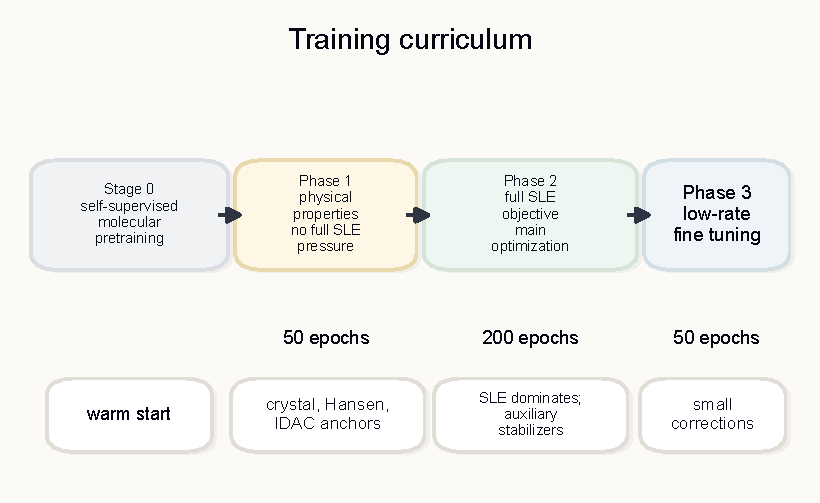
\includegraphics[width=0.94\textwidth]{training_curriculum_schematic.pdf}
\caption{Поэтапная схема обучения. Она нужна не для усложнения протокола, а для того, чтобы решатель получил физически разумные входы до того, как станет главным источником градиента.}
\label{fig:training-curriculum}
\end{figure}

\textbf{Фаза 1} обучает прежде всего свойства чистого вещества и вспомогательные физические величины: $\Tm$, $\dHfus$, параметры Хансена, а также доступные сигналы активности. Полный SLE-путь ещё не должен доминировать, потому что случайные параметры NRTL в начале обучения способны породить бессмысленные градиенты.

\textbf{Фаза 2} включает основную функцию ошибки по растворимости. Именно здесь модель должна научиться согласовывать кристаллический вклад, активность раствора и итоговый $\ln x_2$. В этой фазе особенно важны мини-пакеты с несколькими температурами одной пары: если в одном мини-пакете есть несколько температур одной пары, можно добавлять ограничения на температурный порядок и локальную форму Вант-Гоффа.

\textbf{Фаза 3} выполняет дообучение с меньшим шагом. Её роль --- не переучивать всю модель, а стабилизировать физические диапазоны, остаточную поправку и поведение на валидации.

Дополнительно поддержаны два режима стабилизации. Первый --- оракульная подстановка во время обучения: если экспериментальные $\Tm$ или $\dHfus$ известны, они иногда временно подаются в решатель вместо предсказанных значений. Это не используется как основной режим оценки, а служит способом дать NRTL-ветви качественный градиент на ранних этапах. Второй --- заморозка остатка вокруг группового априорного прогноза для кристаллических свойств: если включены групповые оценки $\Tm$ и $\dHfus$, нейросетевая поправка сначала равна нулю и начинает обучаться не сразу.

Вторая фаза использует парно-ориентированную сборку мини-пакетов. Это не техническая мелочь: температурные члены функции ошибки имеют смысл только тогда, когда в одном мини-пакете есть несколько температур одной и той же пары. При случайной сборке строк такие члены часто становятся пустыми или почти пустыми, и модель фактически обучается только точечным значениям. Поэтому в текущем контуре мини-пакеты специально сохраняют повторные температурные наблюдения, чтобы можно было контролировать порядок и наклон кривой внутри пары.

Формально загрузчик старается собирать мини-пакет как объединение малых групп
\begin{equation*}
    B=\bigcup_{(s,v)\in\mathcal P_B}
    \{(s,v,T_j,q_j):T_j\in\mathcal T_{s,v}^{B}\},
\end{equation*}
где хотя бы для части пар $|\mathcal T_{s,v}^{B}|\ge 2$. После этого температурные члены функции ошибки вычисляются только внутри одной пары, а не между химически разными строками. Это особенно важно для \code{pair\_temp\_rank}, \code{vant\_hoff\_local}, компонент наклона и свободного члена, а также якорных строк Вант-Гоффа: без такой сборки эти ограничения превращаются в шум или почти не включаются.

\subsection{Состав функции ошибки}

Полная функция ошибки является суммой основной ошибки растворимости и вспомогательных физических членов:
\begin{equation*}
    \mathcal L
    = \lambda_{\mathrm{sol}}\mathcal L_{\mathrm{sol}}
    + \lambda_{\mathrm{cryst}}\mathcal L_{\mathrm{cryst}}
    + \lambda_{\mathrm{act}}\mathcal L_{\mathrm{act}}
    + \lambda_{\mathrm{temp}}\mathcal L_{\mathrm{temp}}
    + \lambda_{\mathrm{repr}}\mathcal L_{\mathrm{repr}}
    + \lambda_{\mathrm{reg}}\mathcal L_{\mathrm{reg}}.
\end{equation*}
Здесь каждый член включается только там, где для него есть данные или физический смысл. Отсутствующая метка не заменяется нулём: для $\Tm$, $\dHfus$, параметров Хансена и IDAC используются маски.

Основная часть --- робастная ошибка Хьюбера по $\ln x_2$~\cite{huber1964}:
\begin{equation*}
    \mathcal L_{\mathrm{sol}}
    = \rho_\delta\!\left(\widehat{\ln x_2}-\ln x_2\right),
\end{equation*}
где $\rho_\delta$ квадратична около нуля и линейна на больших ошибках. Такой выбор устойчивее MSE для экспериментального корпуса с выбросами, но даёт более гладкий градиент, чем чистая MAE.

Кристаллическая часть связывает выходы модели с известными $\Tm$ и $\dHfus$:
\begin{equation*}
    \mathcal L_{\mathrm{cryst}}
    = m_T\rho(\widehat T_m-T_m)
    + m_H\rho(\widehat{\Delta H}_{\mathrm{fus}}-\Delta H_{\mathrm{fus}}),
\end{equation*}
где $m_T$ и $m_H$ --- маски наличия метки. В энтропийно-согласованном режиме модель предсказывает $\dHfus$ и $\dSfus$, а температуру плавления получает как $\Tm=\dHfus/\dSfus$. Это не гарантирует идеальный прогноз, но не даёт тройке $(\Tm,\dHfus,\dSfus)$ стать термодинамически бессвязной.

Часть активности включает IDAC:
\begin{equation*}
    \mathcal L_{\mathrm{IDAC}}
    = w_{\mathrm{exp}}\rho\!\left(\widehat{\ln\gamma_2^\infty}-\ln\gamma_{2,\mathrm{exp}}^\infty\right)
    + w_{\mathrm{UNIFAC}}\rho\!\left(\widehat{\ln\gamma_2^\infty}-\ln\gamma_{2,\mathrm{UNIFAC}}^\infty\right).
\end{equation*}
Экспериментальные IDAC-данные имеют больший вес, чем UNIFAC-псевдометки. Принципиально, что IDAC подключается отдельным вспомогательным потоком, а не добавляется как строка растворимости: у такой строки нет измеренного SLE-значения $\ln x_2$.

Температурная часть включает мягкие ограничения на монотонность и локальные наклоны Вант-Гоффа. Эти члены не должны становиться главной целью оптимизации: их задача --- удерживать физическую форму кривой, а не заменить экспериментальную ошибку по растворимости. На ранних версиях это ограничение нарушалось: локальный член Вант-Гоффа на шумных или почти плоских температурных сериях мог вырасти с $3811$ до $240148$ и начать доминировать над основной задачей. После этого были добавлены маски корректных пар, ограничение остатка наклона и меньшие фазовые веса. Этот эпизод важен методически: физически правильный штраф может вредить, если его масштаб не согласован с главным экспериментальным сигналом.

Представленческая часть включает параметры Хансена и их парные разности. Индивидуальные $\delta_d$, $\delta_p$, $\delta_h$ полезны, но для растворимости важна именно совместимость двух компонентов, поэтому отдельно подготовлена функция ошибки на разность параметров пары. В TIMP-режиме дисперсионный и полярный каналы также получают слабый обучающий сигнал, чтобы не схлопнуться в одно и то же представление.

Регуляризация ограничивает физические диапазоны параметров: величины $\tau_{12}$ и $\tau_{21}$ не должны уходить в нефизичные значения, $\alpha$ остаётся в допустимом интервале, а остаточная поправка не должна превращать TGNN-Solv в прямую модель. Связующий штраф на основе теории регулярных растворов по умолчанию выключен. Причина не в том, что параметры Хансена бесполезны: дисперсионный и полярный вклады действительно дают полезную меру несовместимости. Ограничение находится в знаке и области применимости: классический вклад Хансена неотрицателен, тогда как специфические контакты, прежде всего водородные связи, могут быть выгодными и приводить к $\gamma_2<1$. Поэтому текущий мостовой компонент сохранён как абляция, а безопасная версия должна быть знако-гибкой поправкой, а не жёстким включением регулярного раствора во все пары.

\begin{figure}[H]
\centering
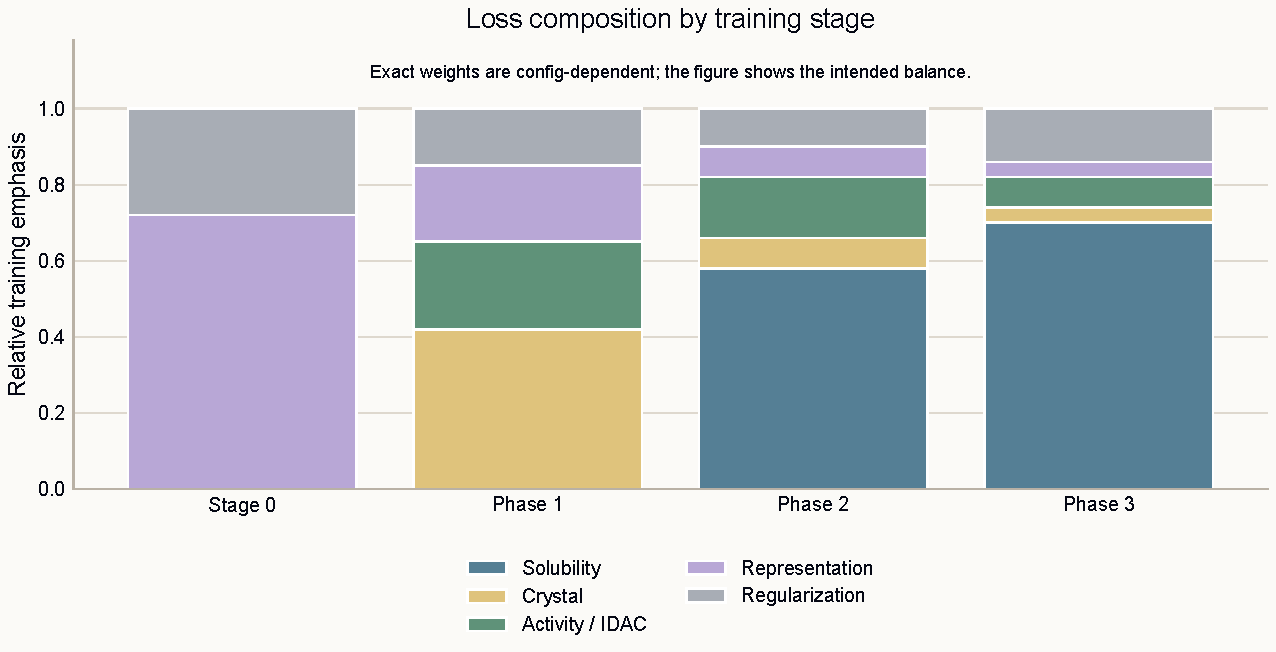
\includegraphics[width=0.86\textwidth]{loss_components_schematic.pdf}
\caption{Состав функции ошибки по этапам. Точные веса задаются конфигурацией, но принцип остаётся неизменным: на второй фазе должна доминировать растворимость, а физические члены должны стабилизировать промежуточные величины, не подменяя главную задачу.}
\label{fig:loss-components}
\end{figure}

Чтобы функция ошибки не выглядела набором независимых добавок, важно сопоставить каждый наблюдаемый сигнал со скрытой величиной, которую он ограничивает. Это сопоставление приведено на рисунке~\ref{fig:supervision-matrix}. Оно показывает главный источник сложности: растворимость ограничивает сразу сумму кристаллического вклада и активности, тогда как прямые наблюдения для NRTL-параметров появляются только через IDAC, UNIFAC-приоры и температурные ряды.

\begin{figure}[H]
\centering
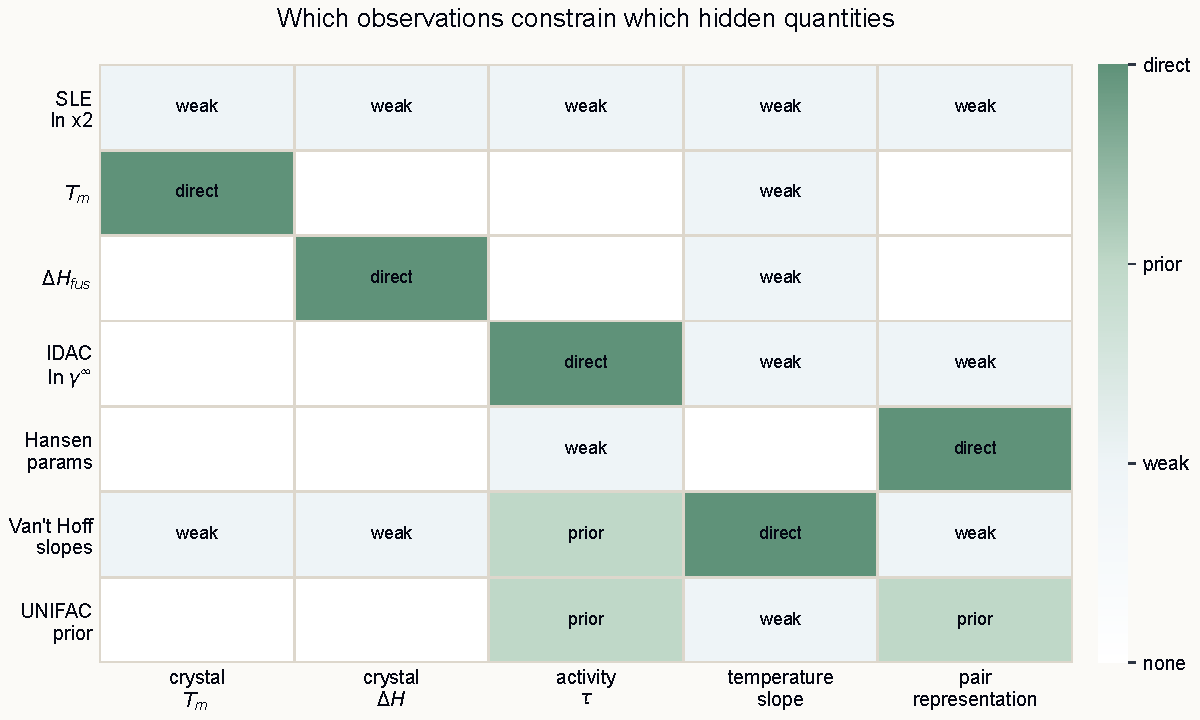
\includegraphics[width=0.90\textwidth]{supervision_matrix.pdf}
\caption{Какие наблюдения ограничивают скрытые величины модели. Такая матрица нужна для понимания идентифицируемости: сильная ошибка по итоговой растворимости сама по себе не гарантирует правильные $T_m$, $\Delta H_{\mathrm{fus}}$ и параметры активности.}
\label{fig:supervision-matrix}
\end{figure}

\begin{table}[H]
\centering
\caption{Основные компоненты функции ошибки и их роль.}
\label{tab:loss-components}
\small
\begin{tabularx}{\textwidth}{P{0.22\textwidth}P{0.24\textwidth}Y}
\toprule
Компонент & Источник сигнала & Зачем нужен \\
\midrule
$\mathcal L_{\mathrm{sol}}$ & измеренные $\ln x_2$ & главная целевая ошибка по растворимости \\
$\mathcal L_{\mathrm{cryst}}$ & $\Tm$, $\dHfus$, групповые оценки & удерживает кристаллический вклад в физически разумной области \\
$\mathcal L_{\mathrm{IDAC}}$ & экспериментальные IDAC и UNIFAC-псевдометки & даёт частичный прямой сигнал на коэффициент активности при бесконечном разбавлении \\
$\mathcal L_{\mathrm{Hansen}}$ & параметры Хансена и парные разности & структурирует представление совместимости молекул \\
$\mathcal L_{\mathrm{temp}}$ & температурные серии одной пары & удерживает форму зависимости $\ln x_2$ от $1/T$ \\
$\mathcal L_{\mathrm{reg}}$ & физические диапазоны параметров & предотвращает вырожденные решения и чрезмерную остаточную поправку \\
\bottomrule
\end{tabularx}
\end{table}

\subsection{Протокол оценки}

Основная метрика --- $\mae$ по $\ln x_2$:
\begin{equation*}
    \mae = \frac{1}{n}\sum_{i=1}^n \abs{\widehat{\ln x_{2,i}}-\ln x_{2,i}}.
\end{equation*}
Также используется $\Rtwo$. Для температурных проверок дополнительно анализируются ошибка наклона $\ln x_2$ как функции $1/T$, правильность направления изменения растворимости с температурой, распределение ошибки по парам и качество формы кривой.

Случайное разбиение строк не используется как главный вывод, потому что в корпусе много повторных измерений одной пары при разных температурах. Если делить строки случайно, одна и та же пара часто попадает и в обучение, и в тест. Такой режим полезен как нижняя оценка сложности, но не отвечает на вопрос о новых веществах.

\section{Основные результаты}

\subsection{Новые молекулярные каркасы}

Основная таблица текущего состояния приведена в таблице~\ref{tab:scaffold-main}.

\begin{table}[H]
\centering
\caption{Основной тест по новым молекулярным каркасам. Все числа в таблице --- один поддерживаемый запуск без доверительных интервалов.}
\label{tab:scaffold-main}
\begin{tabularx}{\textwidth}{P{0.30\textwidth}rrY}
\toprule
Модель & $\mae$ & $\Rtwo$ & Статус \\
\midrule
DirectGNN & 1.652 & 0.478 & лучшая средняя ошибка в этом запуске \\
Случайный лес, гибридные признаки & 1.722 & 0.449 & сильная контрольная модель \\
TGNN-Solv & 1.741 & 0.438 & физический путь в текущей реализации уступает \\
\bottomrule
\end{tabularx}
\end{table}

\begin{figure}[H]
\centering
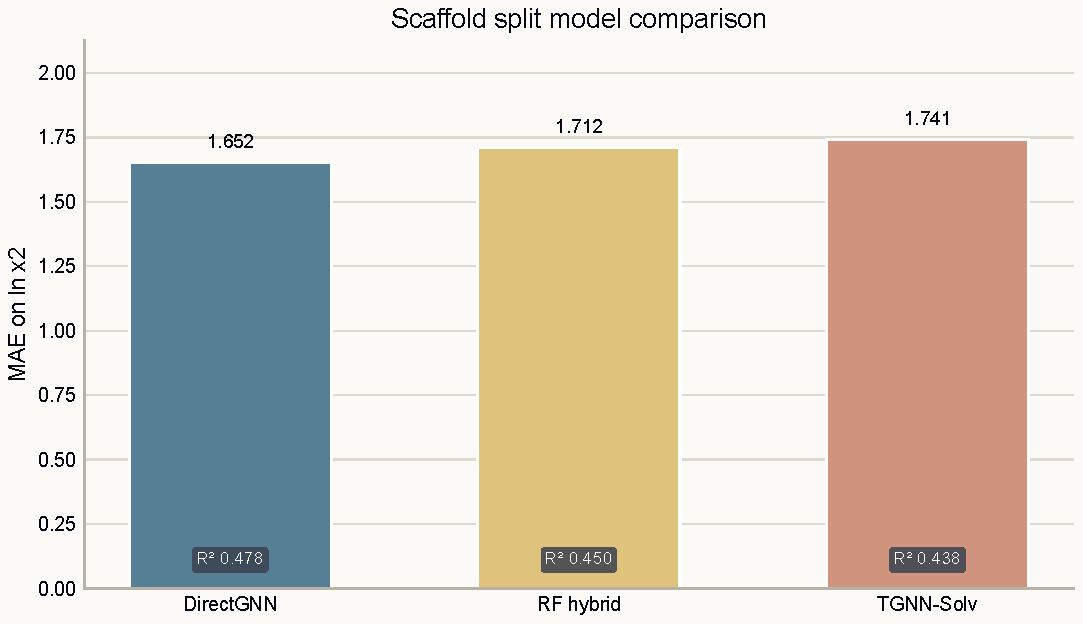
\includegraphics[width=0.88\textwidth]{prediction_slice_model_comparison.pdf}
\caption{Сравнение основных моделей на текущем наборе диагностических срезов. Рисунок показывает как общий проигрыш TGNN-Solv по MAE, так и неоднородность этого проигрыша по химическим областям.}
\label{fig:model-comparison}
\end{figure}

Разница TGNN-Solv и DirectGNN составляет $0.089$ по MAE. Для текущей стадии это важный отрицательный результат: термодинамически ограниченный путь не даёт выигрыша по средней ошибке на разбиении по новым каркасам. При этом статистическую значимость разрыва ещё нельзя утверждать: для неё нужны независимые инициализации и доверительный интервал, а не один запуск. Значение $\Rtwo=0.478$ у лучшей текущей модели также не является сильным качеством в абсолютном смысле: оно означает, что на новых каркасах объясняется меньше половины дисперсии целевой величины.

Однако это не означает, что физическая модель является просто ухудшенной копией прямой. В парном сравнении TGNN-Solv лучше DirectGNN примерно на $46.4\%$ строк и $46.9\%$ пар. Кроме того, у TGNN-Solv меньше доля пар с очень большой средней ошибкой выше $3.0$: $15.4\%$ против $17.1\%$ у DirectGNN. Значит, модели имеют разную структуру ошибок.

\begin{figure}[H]
\centering
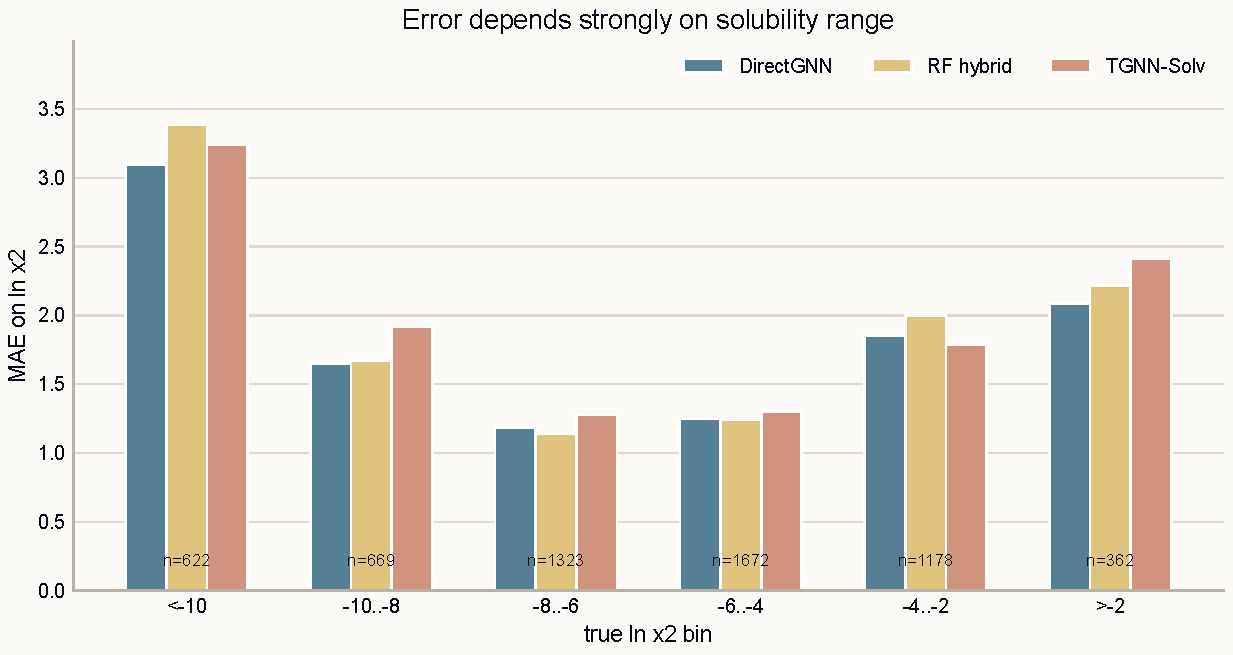
\includegraphics[width=0.90\textwidth]{prediction_slice_lnx2_bin_mae.pdf}
\caption{Ошибка как функция истинной растворимости на каркасном тесте. Левый хвост очень плохо растворимых систем является одним из главных источников ошибки, особенно для TGNN-Solv: именно там слабый вклад активности раствора приводит к завышению растворимости.}
\label{fig:lnx2-bin-mae}
\end{figure}

Этот срез важнее, чем ещё одна общая метрика: он показывает, что ошибка неоднородна по диапазону $\ln x_2$. Если модель сжимает предсказания к центру распределения, она может выглядеть приемлемо по средней ошибке, но систематически проваливать вещества с очень низкой растворимостью.

\subsection{Трудные зарядовые и постановочные случаи}

После разбора крайних примеров была добавлена отдельная диагностика трудных систем, а не архитектурное усложнение по умолчанию. Скрипт \code{scripts/analysis/audit_difficult_ionic_systems.py} классифицирует строки по формальному заряду, числу фрагментов, признаку соли, цвиттер-ионности и грубому режиму диэлектрической проницаемости растворителя. Это важно методически: строка с заряженным SMILES в этаноле или ацетоне не обязательно требует eNRTL, потому что при низкой диэлектрической проницаемости она может вести себя как контактная ионная пара. Напротив, заряженная система в воде или ДМСО уже ближе к настоящей электролитной постановке.

\begin{figure}[H]
\centering
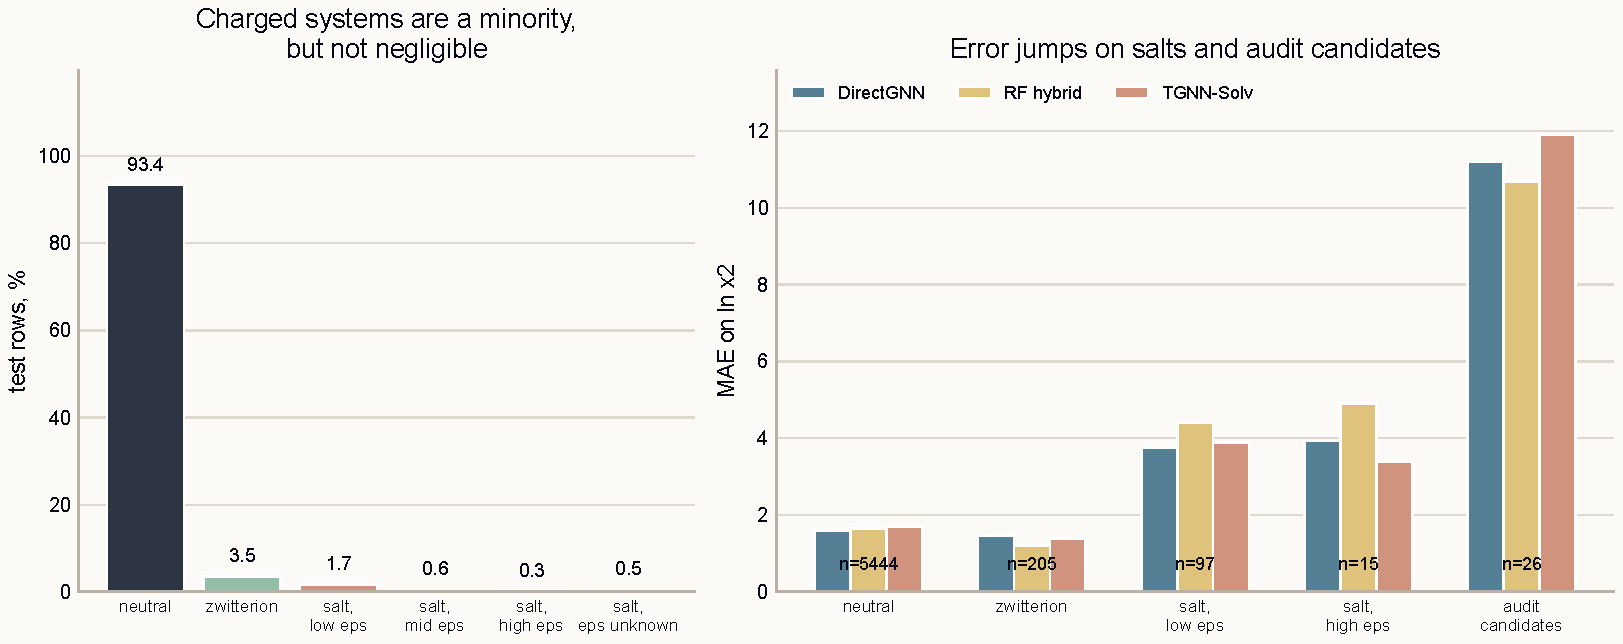
\includegraphics[width=0.96\textwidth]{difficult_systems_audit_summary.pdf}
\caption{Аудит трудных систем на каркасном тесте. Зарядовые системы являются меньшинством, но ошибка на них резко выше средней. Кандидаты на ручной аудит --- это экстремально плохо растворимые заряженные или антоцианидин-подобные строки, где проблема может быть не только модельной, но и постановочной.}
\label{fig:difficult-system-audit}
\end{figure}

Численно в основном тесте $6.6\%$ строк имеют формальный заряд, $3.6\%$ являются явными солями, $3.5\%$ --- цвиттер-ионами. Кандидаты на режим контактных ионных пар в низкодиэлектрических растворителях составляют $3.0\%$ тестовых строк, а кандидаты на настоящую диссоциацию в высокодиэлектрических растворителях --- $0.9\%$. Это не маргинальный эффект, но и не всё объяснение средней ошибки: нейтральные системы остаются основной массой корпуса.

На существующих предсказаниях ошибка DirectGNN на нейтральных строках равна $\mae=1.604$, а на всех зарядовых строках --- $\mae=2.337$. Для TGNN-Solv соответствующие значения равны $1.701$ и $2.309$. На явных солях в низкодиэлектрических растворителях ошибка ещё выше: $3.749$ для DirectGNN и $3.894$ для TGNN-Solv. На $26$ строках, помеченных как кандидаты на ручной аудит постановки, ошибка становится катастрофической: $11.19$ и $11.90$ соответственно. Это сильный аргумент против немедленного перехода к eNRTL: сначала нужно отделить физически корректные сложные системы от строк, где эксперимент мог относиться к смеси растворителей, подкисленной среде, другой солевой форме или полиморфу.

Пример дельфинидин-хлорида подтверждает эту осторожность, но уточняет её. В обработанном каркасном тесте есть $40$ строк: ацетон, этанол, метанол и вода по $10$ температурных точек. Для ацетона диапазон $\ln x_2$ равен $-23.62$--$-22.57$, для этанола $-16.67$--$-15.67$, для метанола $-14.35$--$-13.29$, для воды $-14.44$--$-13.32$. Эти строки соответствуют работе Kumoro et al.~\cite{kumoro2010}: растворимость дельфинидина измерялась спектрофотометрически в воде, метаноле, этаноле и ацетоне при $298.15$--$343.15\,\mathrm K$, а материалы описаны как вода, абсолютный этанол, безводный метанол и ацетон, использованные как растворители без дополнительной очистки. Поэтому гипотеза о подкисленной смеси для этого конкретного источника не подтверждается.

\begin{figure}[H]
\centering
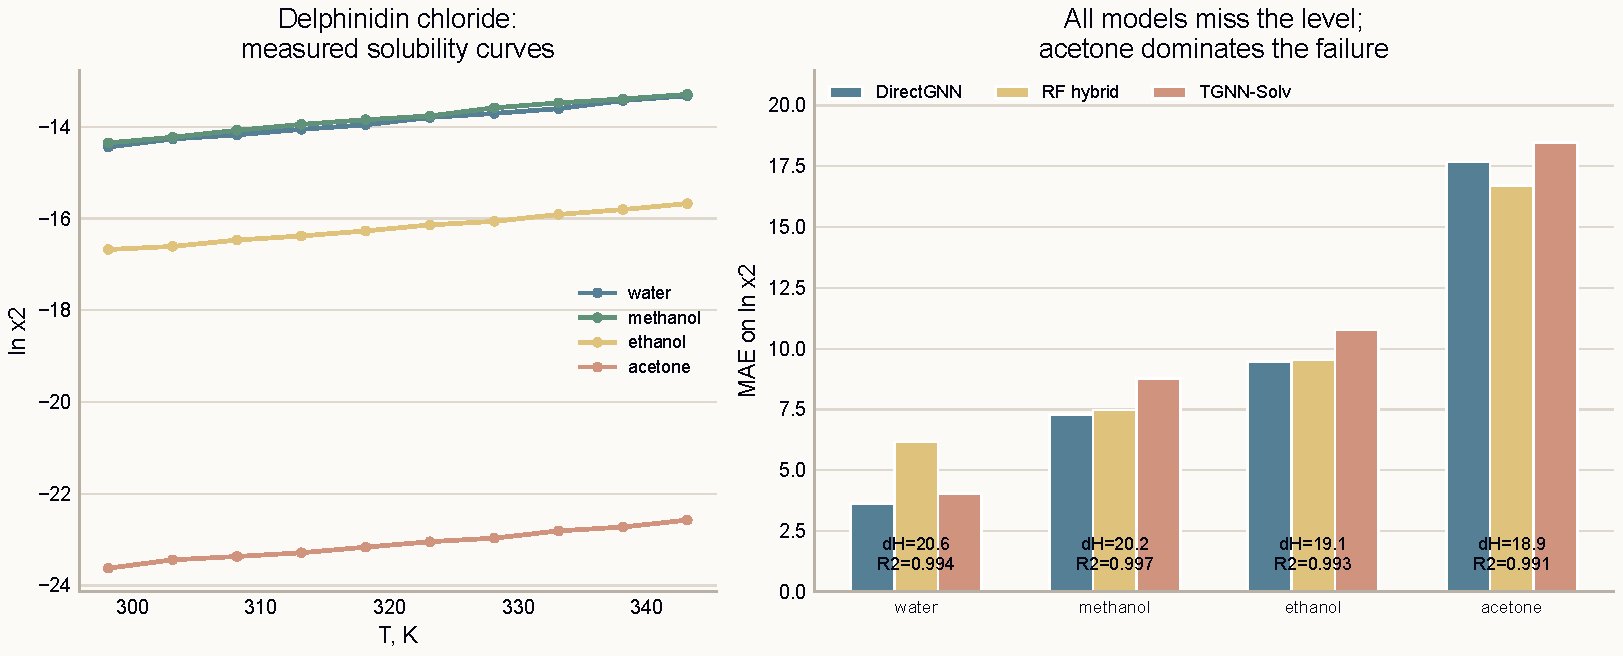
\includegraphics[width=0.96\textwidth]{delphinidin_case_study.pdf}
\caption{Дельфинидин-хлорид как локальный разбор экстремального хвоста. Слева показаны экспериментальные температурные кривые: во всех четырёх растворителях растворимость монотонно растёт с температурой, а линейная аппроксимация Вант-Гоффа имеет $R^2>0.991$. Справа показано, что модели ошибаются в основном в уровне кривой, особенно для ацетона и этанола.}
\label{fig:delphinidin-case-study}
\end{figure}

Именно дельфинидин даёт $20$ из $26$ строк, помеченных как кандидаты на ручной аудит: это ацетоновые и этаноловые точки с $\ln x_2<-15$. Ошибка всех моделей здесь систематически положительная, то есть модели завышают растворимость. Для ацетона MAE равна $17.68$ у DirectGNN, $16.72$ у RF-гибрида и $18.47$ у TGNN-Solv; для этанола --- $9.48$, $9.53$ и $10.77$ соответственно. Метанол и вода тоже трудны, но уже не попадают в самый экстремальный срез: для воды DirectGNN имеет $\mae=3.63$, TGNN-Solv --- $4.03$.

Температурные наклоны у дельфинидина выглядят физически согласованно: эффективная энтальпия растворения из наклона Вант-Гоффа составляет примерно $18.9$--$20.6\,\mathrm{kJ/mol}$, а растворимость монотонно растёт с температурой во всех растворителях. Это снижает вероятность простой ошибки знака или единиц в температурной серии. Главная незакрытая часть --- кристалл: в обработанных строках нет экспериментальных $T_m$ и $\Delta H_{\mathrm{fus}}$, поэтому требуемую $\ln\gamma_2^{\mathrm{req}}$ через контрольный расчёт с известными кристаллическими параметрами посчитать нельзя. Следовательно, дельфинидин остаётся примером экстремального хвоста и особой химии антоцианидиновой соли, но не является самостоятельным доказательством необходимости электролитного NRTL.

Отдельный расчёт $\ln\gamma_2^{\mathrm{req}}$ возможен только для строк, где одновременно есть $T_m$ и $\Delta H_{\mathrm{fus}}$. Таких строк в текущих обработанных CSV всего $1080$, и они находятся в обучающей части. Для них медианное $|\ln\gamma_2^{\mathrm{req}}|$ равно $0.47$, а доля строк с $|\ln\gamma_2^{\mathrm{req}}|>4$ равна $2.9\%$. Это показывает, что экстремальная требуемая неидеальность существует, но она редка и должна рассматриваться как сигнал к аудиту данных, а не как автоматическое требование расширять физическую модель.

\begin{table}[H]
\centering
\caption{Что уже известно по разным режимам разбиения. Полная матрица всех нейросетевых моделей по всем разбиениям ещё не закрыта; строки ниже отделяют готовые артефакты от отсутствующих запусков.}
\label{tab:split-wise-current}
\small
\begin{tabularx}{\textwidth}{P{0.24\textwidth}P{0.21\textwidth}P{0.21\textwidth}Y}
\toprule
Режим проверки & DirectGNN & TGNN-Solv & Доступный ориентир \\
\midrule
Случайные строки & нет финального артефакта & нет финального артефакта & RF: $\mae=0.166$, $\Rtwo=0.987$ \\
Новые пары & нет финального артефакта & нет финального артефакта & RF: $\mae=0.783$, $\Rtwo=0.806$ \\
Новый растворитель & нет финального артефакта & нет финального артефакта & RF: $\mae=0.732$, $\Rtwo=0.735$ \\
Новое вещество & нет финального артефакта & нет финального артефакта & RF: $\mae=1.642$, $\Rtwo=0.420$ \\
Новый каркас & $\mae=1.652$, $\Rtwo=0.478$ & $\mae=1.741$, $\Rtwo=0.438$ & RF-гибрид: $\mae=1.722$, $\Rtwo=0.449$ \\
\bottomrule
\end{tabularx}
\end{table}

Чтобы не смешивать факты, диагностику и рабочие гипотезы, текущий статус проекта полезно формулировать в виде карты доказательности. В ней отдельно отмечено, что уже подтверждено численно, что является диагностическим выводом и что требует полноразмерных запусков.

\begin{figure}[htbp]
\centering
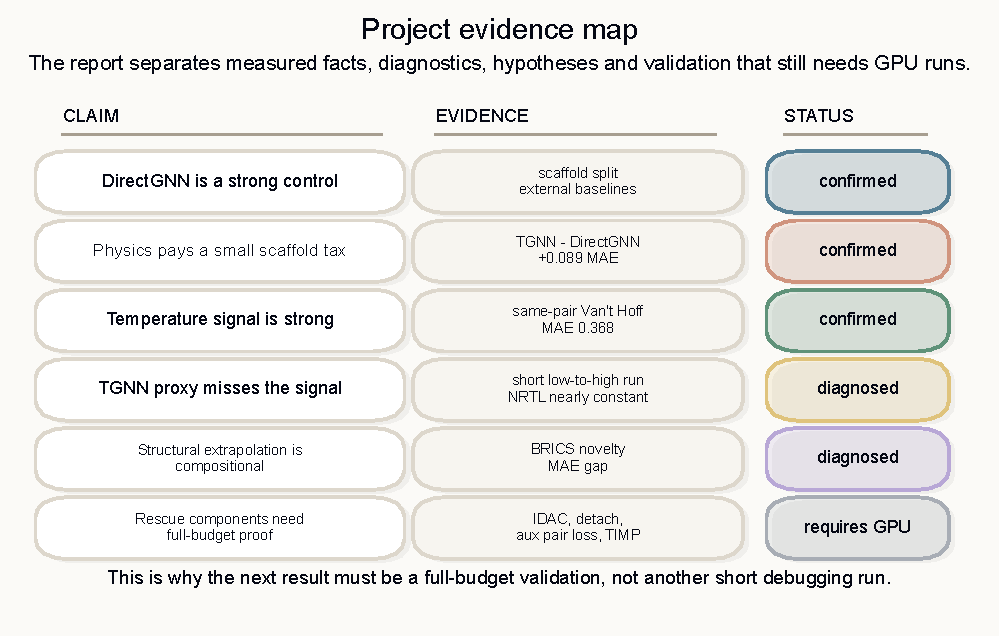
\includegraphics[width=0.82\textwidth]{evidence_status_matrix.pdf}
\caption{Карта доказательности текущих утверждений. Она отделяет воспроизводимые факты от рабочих гипотез и показывает, почему следующий критический шаг --- не новая архитектурная идея, а полноразмерная проверка уже реализованных стабилизирующих компонентов.}
\label{fig:evidence-status}
\end{figure}

\begin{figure}[H]
\centering
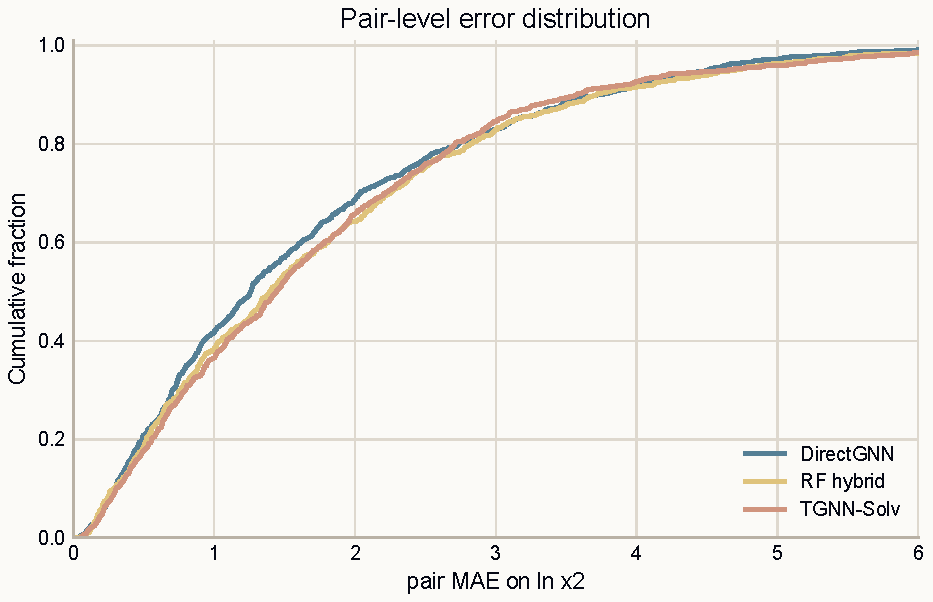
\includegraphics[width=0.64\textwidth]{prediction_slice_pair_mae_cdf.pdf}
\caption{Распределение парных ошибок для основных моделей. Форма распределения важна не меньше среднего значения: часть моделей имеет близкую MAE, но разную долю тяжёлых провалов.}
\label{fig:pair-mae-cdf}
\end{figure}

\begin{figure}[H]
\centering
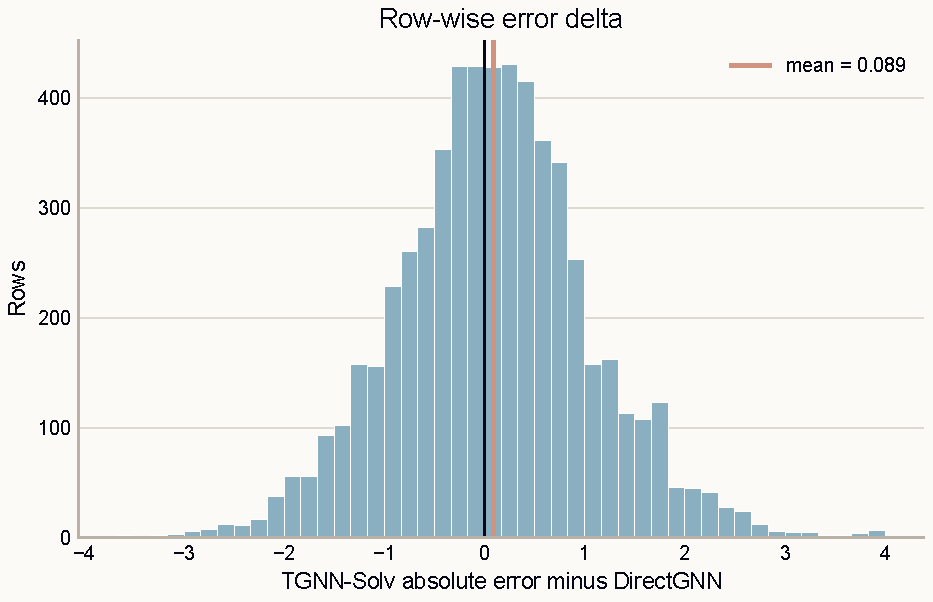
\includegraphics[width=0.64\textwidth]{prediction_slice_paired_deltas.pdf}
\caption{Построчное сравнение TGNN-Solv и DirectGNN. TGNN-Solv выигрывает на заметной доле строк, но проигрывает по средней ошибке из-за более крупных локальных ошибок.}
\label{fig:paired-deltas}
\end{figure}

\subsection{Трудность разных режимов обобщения}

Сравнение разных разбиений на модели случайного леса показывает, насколько сильно протокол оценки влияет на результат.

\begin{table}[H]
\centering
\caption{Сложность разных разбиений по RF-ориентиру.}
\label{tab:splits}
\begin{tabular}{lrrl}
\toprule
Разбиение & $\mae$ & $\Rtwo$ & Интерпретация \\
\midrule
Случайные строки & 0.166 & 0.987 & почти повторение известных пар \\
Случайные пары & 0.783 & 0.806 & новые пары, но знакомые компоненты \\
Новый растворитель & 0.732 & 0.735 & перенос по растворителю относительно легче \\
Новое вещество & 1.642 & 0.420 & трудный перенос на новое вещество \\
Новый каркас & 1.703 & 0.462 & новый каркас и смещение распределения \\
\bottomrule
\end{tabular}
\end{table}

Основная сложность задачи --- новое растворяемое вещество и особенно новый структурный каркас. Это общий вывод для всех проверенных подходов, а не только для TGNN-Solv.

\subsection{Сравнение с внешними моделями}

Внешние модели используются не как главный контроль физического слоя, а как практическая шкала качества. SolProp важен как опубликованная модель для широкого набора растворителей и температур~\cite{vermeire2022}. FastSolv важен как современный быстрый предиктор органической растворимости, обученный в близкой по духу постановке на больших корпусах растворимости~\cite{fastsolv2025}.

SolProp в режиме \emph{дообучения на целевых величинах TGNN-Solv} показал на разбиении по новым веществам $\mae=1.624$ и $\Rtwo=0.388$. Это не внешнее нулевое сравнение с опубликованными весами, а дообученный SolProp в нашем контракте данных. DirectGNN на сопоставимой задаче имеет $\mae=1.652$ и $\Rtwo=0.478$. Таким образом, дообученный SolProp немного лучше по MAE, но DirectGNN лучше по объяснённой дисперсии.

FastSolv потребовал отдельного аудита преобразования единиц. Изначально возникала проблема с нечисловыми предсказаниями из-за некорректных $\log S$-целей после преобразования. После фильтрации нечисловых значений и исправления обработки плотностей модель запускается корректно, но остаётся слабее: на разбиении по новым веществам $\mae=1.941$ и $\Rtwo=0.226$.

Главный вывод из этого блока: DirectGNN находится на уровне сильных внешних ориентиров, поэтому отставание TGNN-Solv нельзя списать на слабую инфраструктуру данных или графового кодирования. Проблема локализуется именно в физическом пути: в идентификации кристаллических параметров, параметров активности и их совместном обучении.

\subsection{Проверка моделируемости данных}

Для проверки, не является ли корпус слишком шумным или случайным, был выполнен поиск ближайшего обучающего примера по химическому сходству. Простейший ближайший сосед дал $\mae=2.530$ и $\Rtwo=-0.192$. Это намного хуже DirectGNN, случайного леса и TGNN-Solv. Следовательно, обучаемые модели действительно извлекают закономерности, которые не сводятся к копированию ближайшего примера.

\begin{figure}[H]
\centering
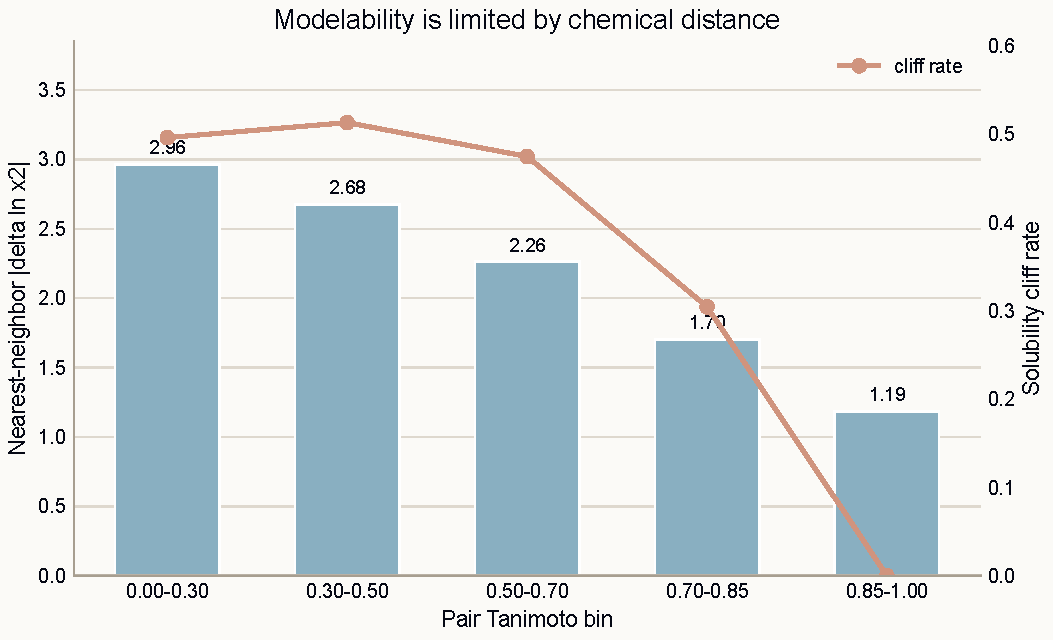
\includegraphics[width=0.90\textwidth]{knn_modelability_diagnostics.pdf}
\caption{Диагностика моделируемости через ближайшего соседа. Даже при росте сходства по коэффициенту Танимото средняя ошибка ближайшего обучающего примера остаётся заметной; локальные скачки растворимости исчезают только в очень близком диапазоне. Это объясняет, почему структурная экстраполяция остаётся трудной даже для сильных моделей.}
\label{fig:knn-modelability}
\end{figure}

Этот результат важен для интерпретации всего проекта. Если бы ближайший сосед уже давал ошибку на уровне $1.6$, сложная модель была бы в основном механизмом поиска похожей записи. В реальности ближайший сосед существенно хуже, а доля «обрывов растворимости» остаётся высокой при умеренном сходстве. Значит, данные содержат переносимые закономерности, но они не сводятся к простой локальной гладкости химического пространства.

\section{Температурные эксперименты}

\subsection{Экстраполяция с низких температур на высокие}

Температура --- режим, где физическая модель должна иметь естественное преимущество~\cite{apelblat1999,hildebrand1970}. Если для одной и той же пары вещество--растворитель известны несколько низкотемпературных точек, зависимость $\ln x_2$ от $1/T$ часто близка к линейной. Это следует из уравнения Вант-Гоффа и родственных термодинамических приближений.

В простейшей записи:
\begin{equation*}
    \ln x_2 \approx a + b\frac{1}{T},
    \qquad
    b \approx -\frac{\Delta H_{\mathrm{sol}}}{R}.
\end{equation*}
Поэтому температурный тест проверяет не только точечную ошибку, но и физический наклон кривой. Если TGNN-Solv действительно использует термодинамическую форму, она должна восстанавливать направление и величину изменения $\ln x_2$ по $1/T$, а не просто давать близкое среднее значение в диапазоне обучения.

Были выбраны пары с несколькими точками при $T\le 310\,\mathrm{K}$ и хотя бы одной точкой при $T\ge 330\,\mathrm{K}$. Низкотемпературные точки используются для обучения или подгонки, высокотемпературные --- для проверки. Итоговый набор содержит $1\,751$ пару, $7\,120$ обучающих строк, $1\,751$ валидационную строку и $3\,343$ тестовые строки. Диапазон тестовых температур --- от $330.0$ до $425.77\,\mathrm{K}$.

После дополнительного аудита этот протокол нужно формулировать точнее: это не проверка на новые пары и не проверка на новые молекулярные каркасы. Все $1\,751$ пары из высокотемпературного теста присутствуют в низкотемпературной части. Поэтому температурная экстраполяция является режимом \emph{той же пары}: она проверяет перенос по температуре при известной паре вещество--растворитель. Это полезный и физически важный режим, но его нельзя смешивать с основным разбиением по новым каркасам.

\begin{table}[H]
\centering
\caption{Аудит протокола низкая температура $\to$ высокая температура.}
\label{tab:temp-protocol-audit}
\small
\begin{tabularx}{\textwidth}{Y r}
\toprule
Показатель & Значение \\
\midrule
Уникальные пары в низкотемпературной обучающей, валидационной и высокотемпературной тестовой частях & $1\,751$ в каждой части \\
Пересечение пар между низкотемпературной обучающей и высокотемпературной тестовой частями & $1\,751/1\,751=100.0\%$ \\
Число строк в обучающей, валидационной и тестовой частях & $7\,120 / 1\,751 / 3\,343$ \\
Доля водных строк в высокотемпературной тестовой части & $12.2\%$ \\
Доля малых растворителей в высокотемпературной тестовой части, $\le 3$ тяжёлых атома & $29.6\%$ \\
Пары с положительным сдвигом $\overline{\ln x_2}_{high}-\overline{\ln x_2}_{low}$ & $99.6\%$ \\
Медианное $R^2$ аппроксимации Вант-Гоффа на низкотемпературных точках & $0.999$ \\
Средняя и медианная ошибка низкотемпературной аппроксимации Вант-Гоффа на высоких температурах & $0.315 / 0.140$ \\
\bottomrule
\end{tabularx}
\end{table}

\begin{figure}[H]
\centering
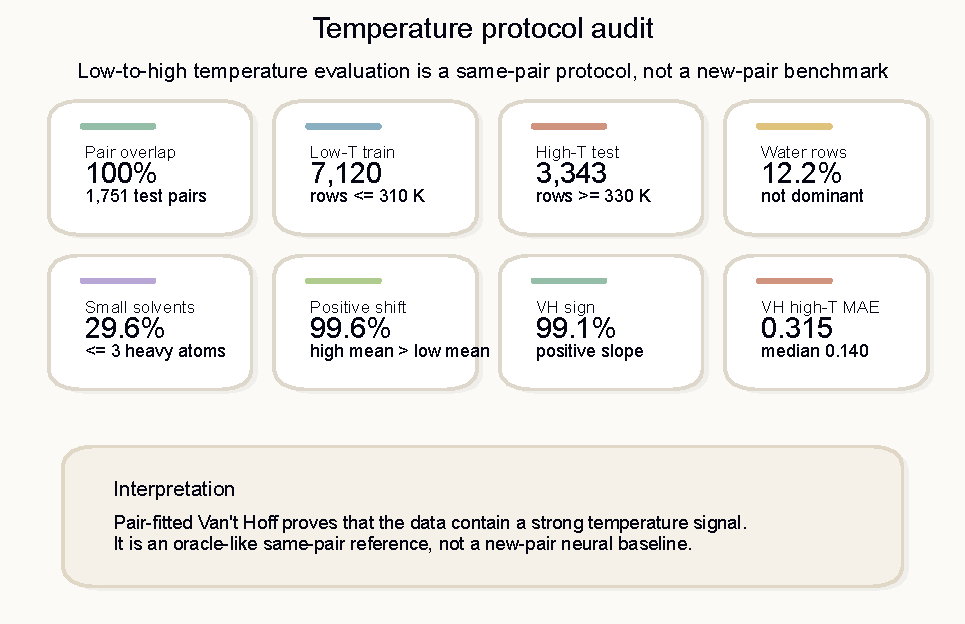
\includegraphics[width=0.92\textwidth]{temperature_protocol_audit.pdf}
\caption{Аудит температурного протокола. Основной вывод: температурная проверка построена корректно как перенос внутри известной пары, а не как тест на новые вещества. Вода присутствует, но не доминирует; направление температурного тренда в данных почти всегда обычное.}
\label{fig:temp-protocol-audit}
\end{figure}

Отдельно важно, что строки этого протокола собраны из объединённых обработанных таблиц, а не сохраняют исходный смысл разбиения по новым каркасам. Например, в train\_low есть строки, которые в исходном корпусе относились к test-разделу. Для данного температурного теста это нормально: здесь единицей проверки является температурная область одной и той же пары. Но эти числа нельзя использовать как доказательство отсутствия или наличия утечки в основном разбиении по новым каркасам.

\begin{table}[H]
\centering
\caption{Диагностическая экстраполяция на высокие температуры для одной и той же пары. Парные аппроксимации Вант-Гоффа являются оракульными ориентирами по известной паре; нейросетевые строки ниже получены в кратких локальных запусках, а не в плановом бюджете.}
\label{tab:temp-extrap}
\begin{tabular}{lrrr}
\toprule
Метод & $\mae$ & $\Rtwo$ & Правильное направление \\
\midrule
Вант-Гофф для каждой пары & 0.368 & 0.887 & 99.0\% \\
Линейная зависимость от $T$ для каждой пары & 0.414 & 0.850 & 99.0\% \\
Последняя низкотемпературная точка & 1.202 & 0.694 & 1.0\% \\
Случайный лес с температурой & 1.290 & 0.658 & 40.4\% \\
Среднее по паре & 1.456 & 0.561 & 1.1\% \\
DirectGNN, краткий локальный запуск & 1.619 & 0.283 & --- \\
TGNN-Solv, краткий локальный запуск & 1.945 & 0.060 & --- \\
\bottomrule
\end{tabular}
\end{table}

\begin{figure}[H]
\centering
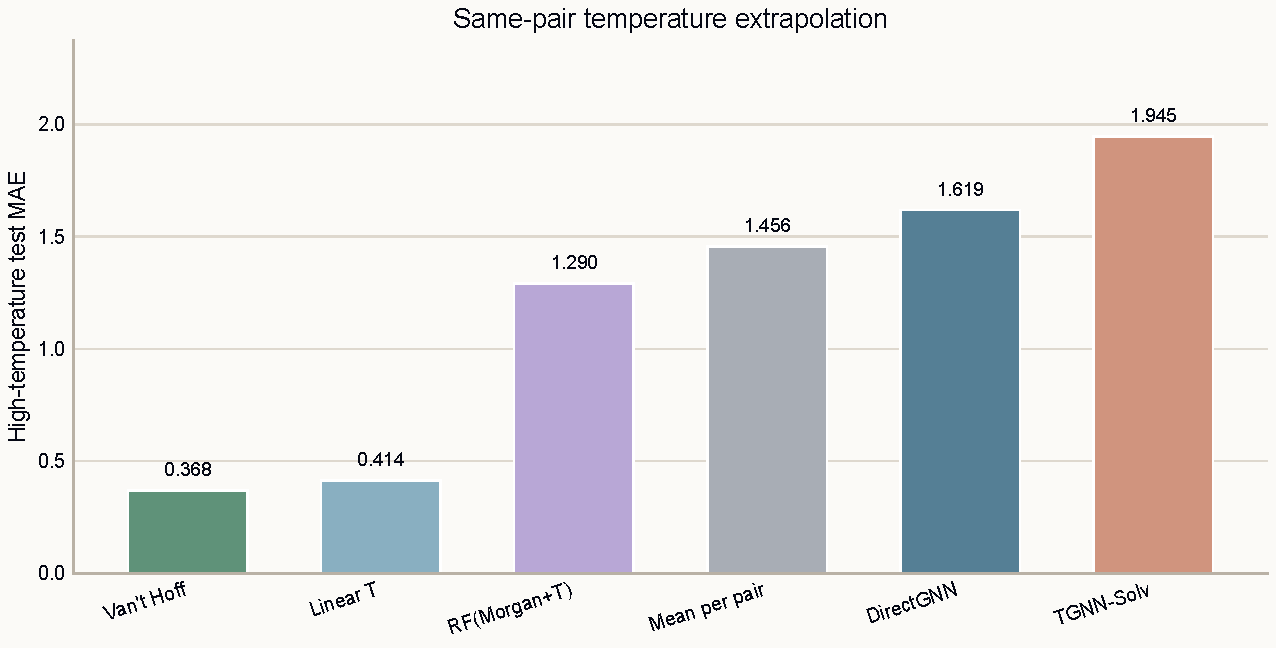
\includegraphics[width=0.88\textwidth]{temperature_extrapolation_baseline_comparison.pdf}
\caption{Температурная экстраполяция на высокие температуры. Простая парная аппроксимация Вант-Гоффа резко лучше кратких нейросетевых запусков, что задаёт главный целевой режим для TGNN-Solv.}
\label{fig:temp-extrap-bars}
\end{figure}

\begin{figure}[H]
\centering
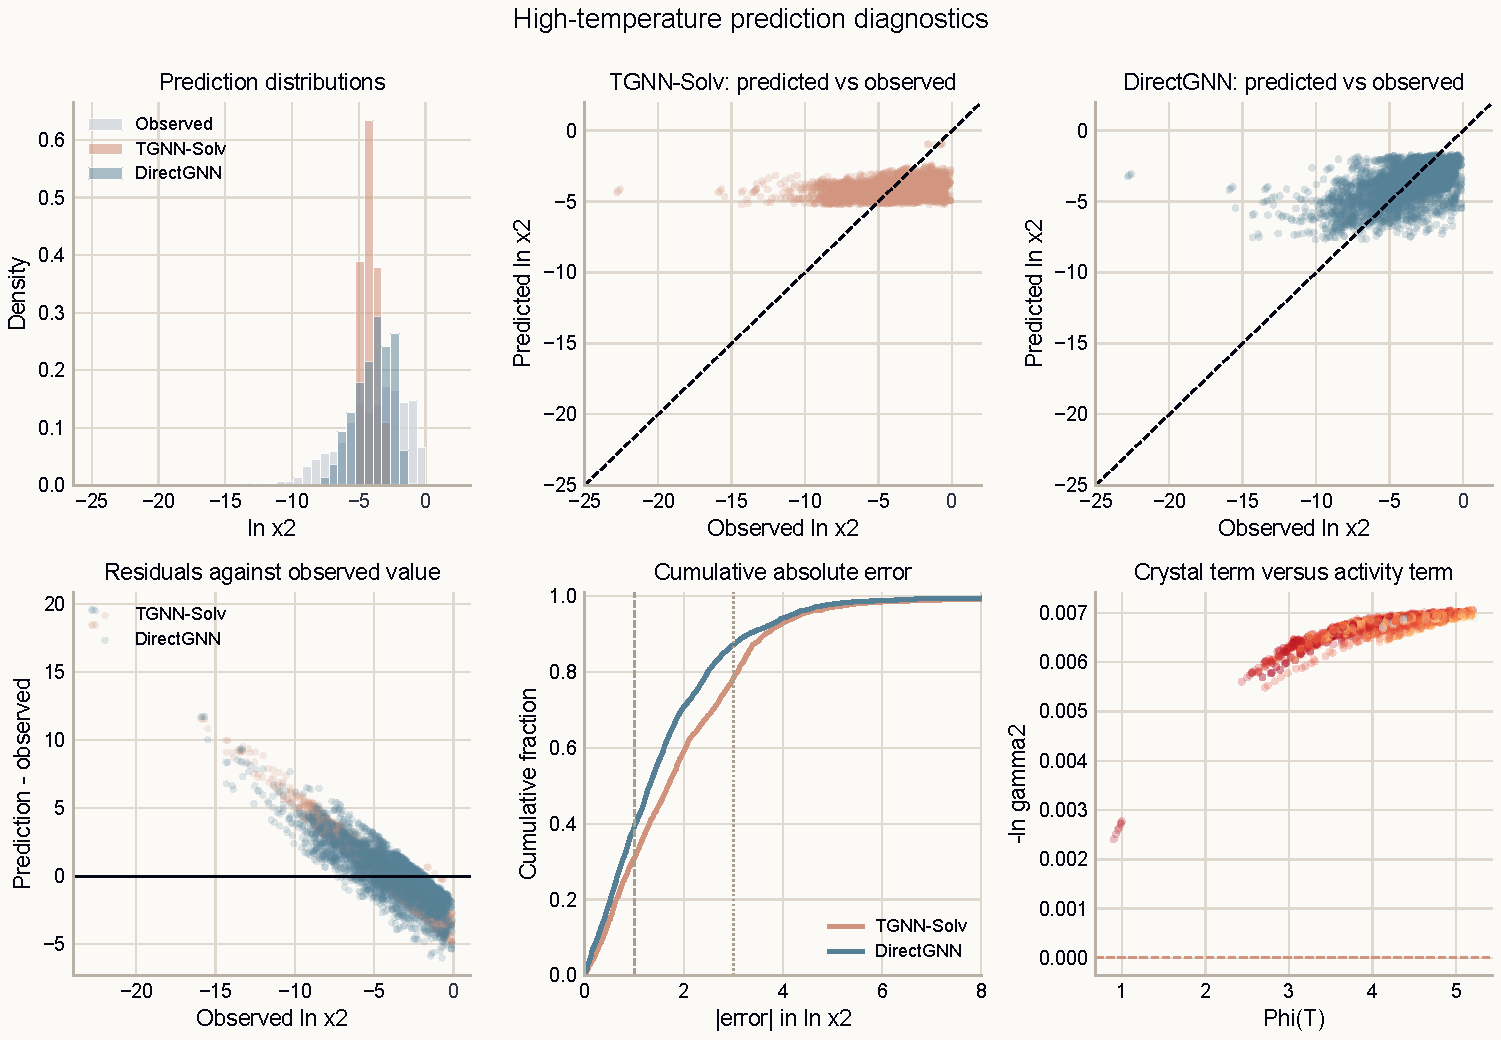
\includegraphics[width=0.96\textwidth]{temperature_prediction_distribution_diagnostics.pdf}
\caption{Распределения и структура ошибок на высокотемпературном тесте. TGNN-Solv в кратком запуске заметно сжимает диапазон предсказаний и хуже воспроизводит левый хвост плохо растворимых систем; это видно одновременно по гистограммам, диаграммам ``предсказание--факт'' и накопленным кривым абсолютной ошибки.}
\label{fig:temp-prediction-distributions}
\end{figure}

Этот рисунок нужен потому, что одних $\mae$ и $\Rtwo$ здесь недостаточно. По распределениям видно не просто то, что TGNN-Solv ошибается сильнее, чем DirectGNN, а то, \emph{как именно} он ошибается: разброс ответов у него уже истинного, а самые низкие значения $\ln x_2$ почти не воспроизводятся. Иными словами, проблема состоит не только в шуме, но и в потере динамического диапазона.

\begin{figure}[H]
\centering
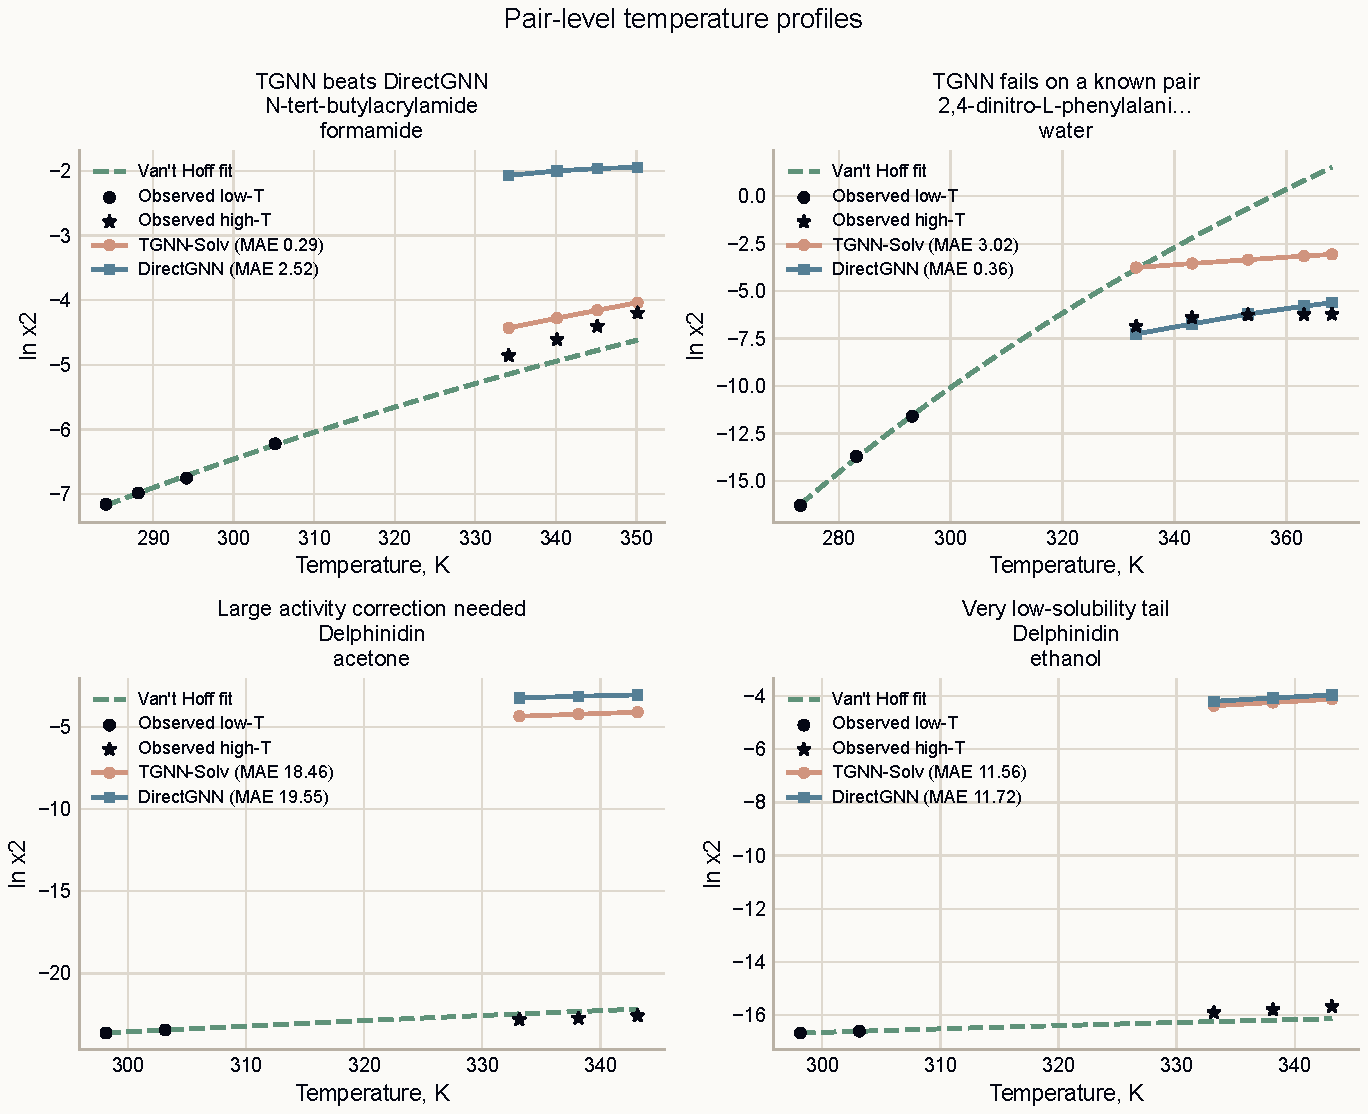
\includegraphics[width=0.94\textwidth]{temperature_pair_profile_panels.pdf}
\caption{Разбор реальных температурных профилей для нескольких известных пар. Панели показывают, что физический путь не бесполезен сам по себе: на части пар TGNN-Solv действительно выигрывает у DirectGNN. Но на других парах, особенно там, где нужен большой вклад активности раствора или наблюдается очень низкая растворимость, краткий запуск физической модели срывается.}
\label{fig:temp-pair-profiles}
\end{figure}

Панели по конкретным парам снимают ещё одну неоднозначность интерпретации. Если смотреть только на усреднённые метрики, легко сделать слишком сильный вывод, будто физическая модель ``не работает вообще''. Это не так. В отчёте теперь есть и пары, где TGNN-Solv действительно лучше прямой модели, и пары, где он резко хуже. Значит, задача состоит не в отказе от физического бутылочного горлышка как идеи, а в том, чтобы понять, при каких химических и температурных режимах оно получает достаточно сигнала. Ниже те же примеры разобраны химически: для каждой системы отдельно показана структура и дано короткое объяснение наблюдаемой ошибки.

\subsection{Химический разбор примерных температурных систем}

\paragraph{N-tert-butylacrylamide--formamide.}
Это нейтральный акриламид с одной амидной донорно-акцепторной группой и объёмным трет-бутильным фрагментом. Formamide --- малый сильнополярный протонный растворитель, поэтому специфическая сольватация амидного центра ожидаема, но требуемая поправка активности в выбранных высокотемпературных точках мала: средний требуемый вклад по диагностике около $0.29$ в $\ln x_2$. Здесь TGNN-Solv выигрывает у DirectGNN ($\mae=0.29$ против $2.52$), потому что физический путь удерживает уровень кривой около наблюдаемого значения. DirectGNN в кратком запуске переоценивает благоприятность полярной пары и предсказывает слишком высокую растворимость.

\begin{figure}[H]
\centering
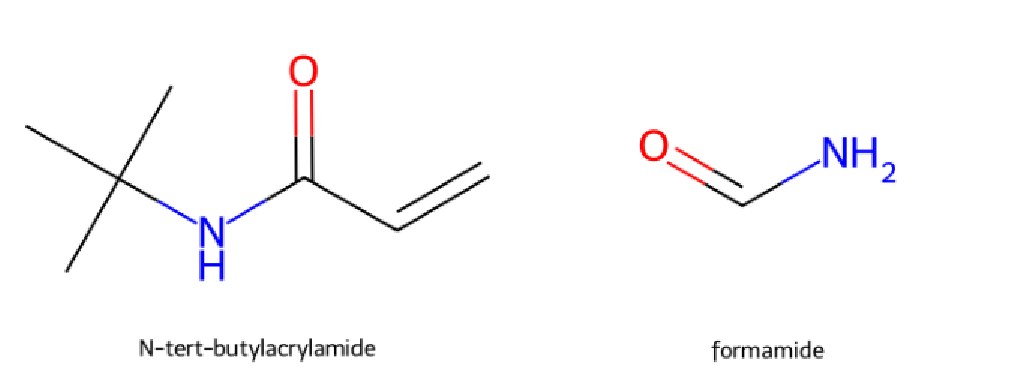
\includegraphics[width=0.58\textwidth]{example_system_n_tert_butylacrylamide_formamide.pdf}
\caption{Структуры пары N-tert-butylacrylamide--formamide. Это пример, где физическое ограничение уровня помогает TGNN-Solv.}
\label{fig:case-n-tert-butylacrylamide-formamide}
\end{figure}

\paragraph{2,4-dinitro-L-phenylalanine--water.}
Эта система противоположна предыдущей. Вещество аминокислотоподобное: есть аминная и карбоксильная функциональность, две сильные нитро-группы и ароматическое ядро. Вода хорошо сольватирует полярные центры, но динитроароматический фрагмент и возможные протонированные/цвиттер-ионные формы делают уровень растворимости нетривиальным. TGNN-Solv здесь сильно завышает растворимость ($\mae=3.02$), тогда как DirectGNN попадает лучше ($\mae=0.36$). Интерпретация простая: краткий физический запуск почти не использует NRTL-ветвь, поэтому не создаёт нужный положительный вклад активности, который должен сдвинуть кривую вниз.

\begin{figure}[H]
\centering
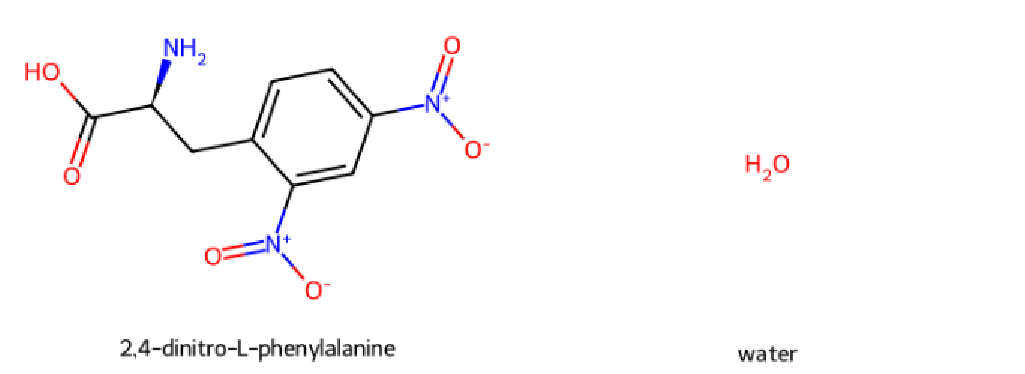
\includegraphics[width=0.58\textwidth]{example_system_2_4_dinitro_l_phenylalanine_water.pdf}
\caption{Структуры пары 2,4-dinitro-L-phenylalanine--water. Ошибка TGNN-Solv связана не с неправильным знаком температурного тренда, а с недостающим уровнем активности.}
\label{fig:case-dinitro-phenylalanine-water}
\end{figure}

\paragraph{Дельфинидин-хлорид--ацетон и дельфинидин-хлорид--этанол.}
Дельфинидин-хлорид --- флавилиевая соль: плоский катионный ароматический хромофор с несколькими фенольными группами и отдельный хлорид-анион. В ацетоне и этаноле это скорее режим контактной ионной пары, а не полностью диссоциированного электролита. При этом в обработанных строках нет экспериментальных $\Tm$ и $\dHfus$, поэтому модель вынуждена восстанавливать кристаллический вклад из необычной соли, которая, вероятно, не имеет обычного плавления. В ацетоне истинные значения лежат около $\ln x_2\approx -23$, а TGNN-Solv ошибается на $18.46$; в этаноле истинные значения около $-16$, ошибка TGNN-Solv равна $11.56$. Это не доказывает необходимость eNRTL само по себе: главная наблюдаемая проблема --- отсутствие корректного кристаллического уровня плюс контактно-ионная сольватация.

\begin{figure}[H]
\centering
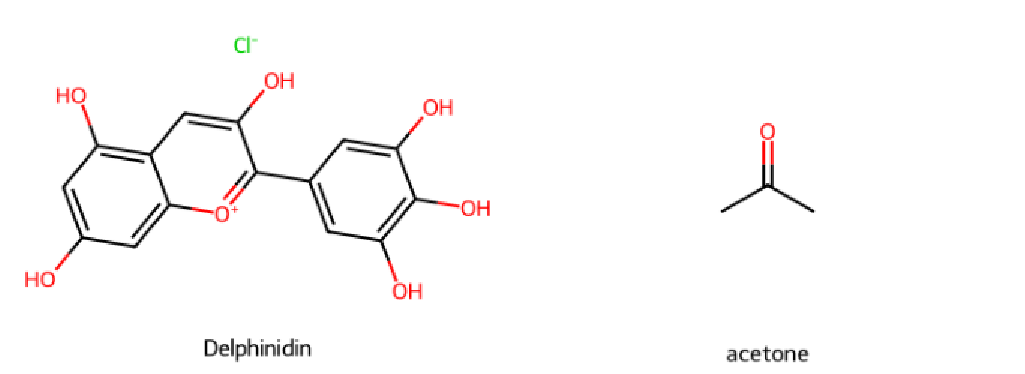
\includegraphics[width=0.58\textwidth]{example_system_delphinidin_acetone.pdf}
\caption{Структуры пары дельфинидин-хлорид--ацетон. Ацетон не даёт сильной протонной стабилизации хлорида; ошибка всех моделей является экстремальным завышением растворимости.}
\label{fig:case-delphinidin-acetone}
\end{figure}

\begin{figure}[H]
\centering
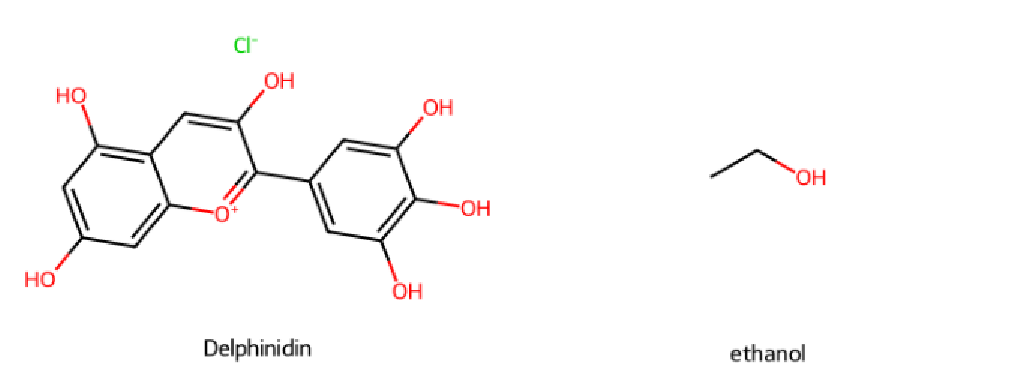
\includegraphics[width=0.58\textwidth]{example_system_delphinidin_ethanol.pdf}
\caption{Структуры пары дельфинидин-хлорид--этанол. Этанол может стабилизировать хлорид водородной связью, но отсутствие кристаллических параметров и солевая форма всё равно делают уровень растворимости трудным.}
\label{fig:case-delphinidin-ethanol}
\end{figure}

\paragraph{Xylitol--toluene.}
Xylitol --- малый полиол с пятью гидроксильными группами. Toluene --- аполярный ароматический растворитель, который не может компенсировать плотную сетку водородных связей полиола. Поэтому истинная растворимость требует большого неблагоприятного вклада активности: полярно-аполярное несоответствие должно сдвигать $\ln x_2$ вниз. TGNN-Solv сохраняет похожий температурный наклон, но завышает уровень кривой примерно на $5.26$. Это типичный случай, где кристаллический член даёт форму, но почти константная NRTL-ветвь не добавляет нужное отталкивание раствора.

\begin{figure}[H]
\centering
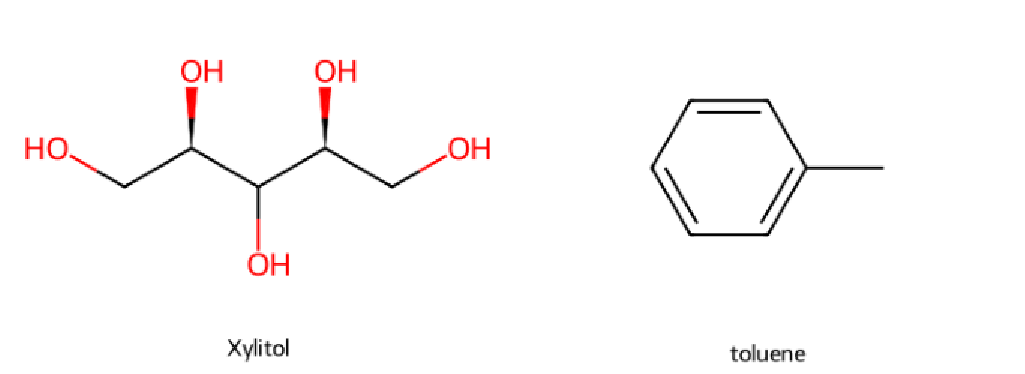
\includegraphics[width=0.58\textwidth]{example_system_xylitol_toluene.pdf}
\caption{Структуры пары xylitol--toluene. Главная химия ошибки --- сильное полярно-аполярное несоответствие.}
\label{fig:case-xylitol-toluene}
\end{figure}

\paragraph{Vitamin K3--benzene.}
Vitamin K3 --- компактный гидрофобный нафтохинон: ароматическая поверхность, два карбонильных акцептора и ограниченная гибкость. Benzene совместим с ним по дисперсионным и $\pi$-взаимодействиям. Здесь ошибка TGNN-Solv имеет другой знак: модель недооценивает растворимость, то есть кривая оказывается слишком низкой. Вероятное объяснение --- физический путь слишком сильно опирается на кристаллический/идеальный вклад и недодаёт благоприятную активностную поправку для ароматического растворителя.

\begin{figure}[H]
\centering
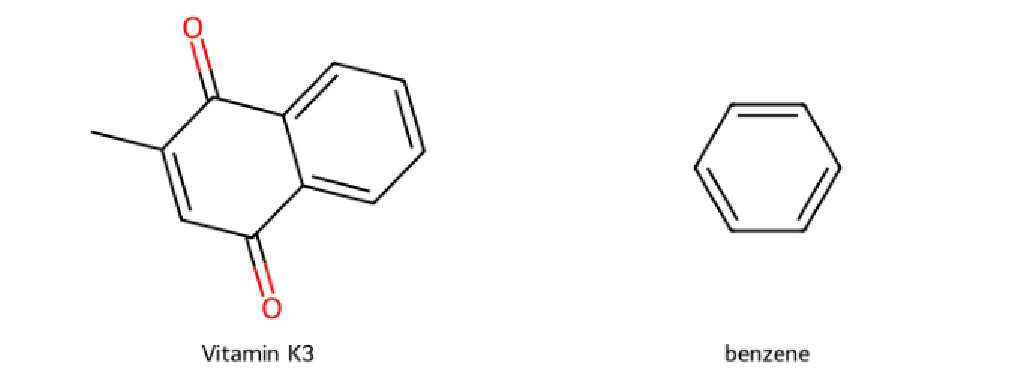
\includegraphics[width=0.58\textwidth]{example_system_vitamin_k3_benzene.pdf}
\caption{Структуры пары Vitamin K3--benzene. Это не левый хвост плохой растворимости, а случай недооценённой совместимости по дисперсионным и ароматическим взаимодействиям.}
\label{fig:case-vitamin-k3-benzene}
\end{figure}

\paragraph{Borneol--p-xylene.}
Borneol --- компактный терпеновый спирт: большая гидрофобная поверхность и один гидроксильный центр. p-Xylene --- аполярный ароматический растворитель, поэтому растворимость в значительной степени определяется дисперсионной совместимостью, а не сильной полярной сольватацией. TGNN-Solv снова предсказывает слишком низкий уровень ($\mae=3.31$ против $1.21$ у DirectGNN). Это указывает не на проблему температурного знака, а на недостающий благоприятный вклад активности для гидрофобно-ароматических пар.

\begin{figure}[H]
\centering
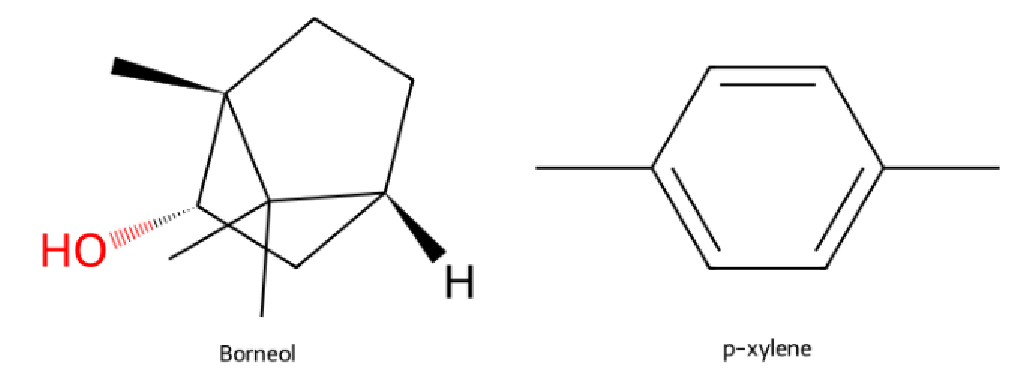
\includegraphics[width=0.58\textwidth]{example_system_borneol_p_xylene.pdf}
\caption{Структуры пары borneol--p-xylene. Ошибка TGNN-Solv связана с недооценкой благоприятной дисперсионной совместимости.}
\label{fig:case-borneol-p-xylene}
\end{figure}

\paragraph{o-Phthalic acid--DMAc.}
o-Phthalic acid содержит две карбоксильные группы в орто-положении и может образовывать сильные меж- и внутримолекулярные водородные связи. DMAc --- полярный апротонный растворитель с сильной карбонильной акцепторной группой. Наблюдаемая растворимость чувствительна к кислотно-основной и донорно-акцепторной ассоциации, а не только к общей полярности. TGNN-Solv недооценивает уровень растворимости: вероятно, кристаллический штраф или идеальная часть слишком велики, а благоприятная acid--amide сольватация не выражена в NRTL-параметрах.

\begin{figure}[H]
\centering
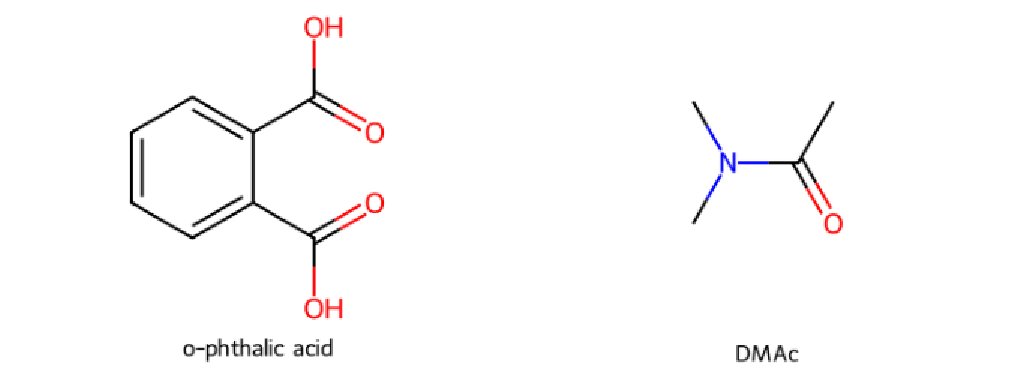
\includegraphics[width=0.58\textwidth]{example_system_o_phthalic_acid_dmac.pdf}
\caption{Структуры пары o-phthalic acid--DMAc. Система показывает чувствительность уровня растворимости к специфической acid--amide ассоциации.}
\label{fig:case-o-phthalic-acid-dmac}
\end{figure}

\paragraph{m-Methylbenzoic acid--isobutanol.}
m-Methylbenzoic acid сочетает гидрофобное ароматическое кольцо и одну сильную карбоксильную группу. Isobutanol может и отдавать, и принимать водородные связи, а также имеет гидрофобный фрагмент. Это химически совместимая acid--alcohol пара. TGNN-Solv недооценивает растворимость примерно на $3.23$ в $\ln x_2$, что согласуется с той же причиной: ветвь активности не добавляет достаточно благоприятного вертикального сдвига для специфической ассоциации кислоты со спиртом.

\begin{figure}[H]
\centering
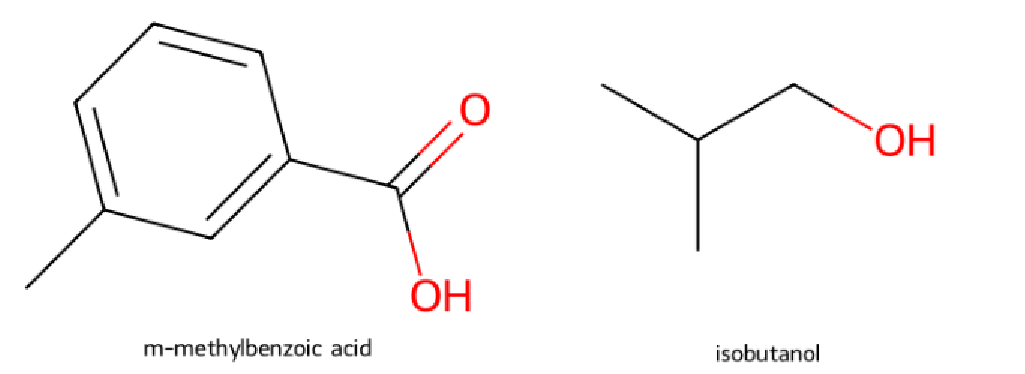
\includegraphics[width=0.58\textwidth]{example_system_m_methylbenzoic_acid_isobutanol.pdf}
\caption{Структуры пары m-methylbenzoic acid--isobutanol. Здесь важны acid--alcohol взаимодействия и гидрофобная совместимость.}
\label{fig:case-m-methylbenzoic-acid-isobutanol}
\end{figure}

\paragraph{Glutaric acid--acetic acid.}
Glutaric acid --- гибкая алифатическая дикарбоновая кислота, а acetic acid одновременно растворитель и участник кислотных ассоциаций. В таких системах уровень растворимости может сильно меняться из-за димеризации, кислотно-кислотных контактов и конкуренции с кристаллической упаковкой. TGNN-Solv держит температурную форму лучше, чем абсолютный уровень: ошибка $3.12$ в основном является вертикальным сдвигом. Это ещё один пример того, что краткий физический запуск знает направление температурной кривой, но не имеет достаточно выразительной активности раствора.

\begin{figure}[H]
\centering
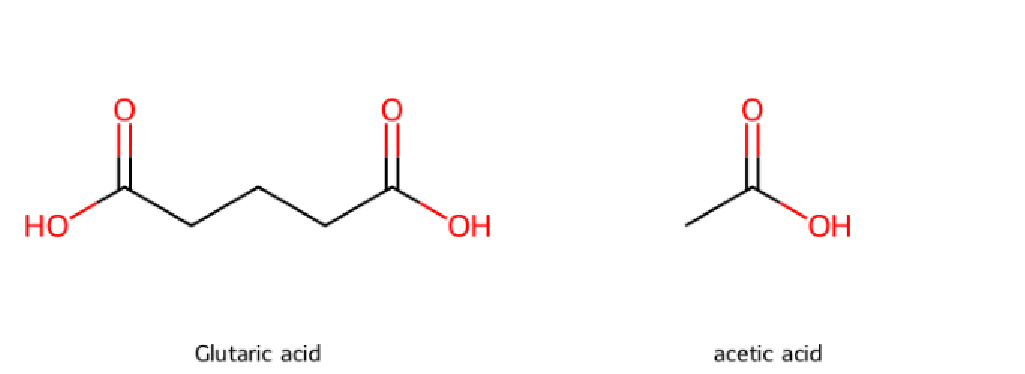
\includegraphics[width=0.58\textwidth]{example_system_glutaric_acid_acetic_acid.pdf}
\caption{Структуры пары glutaric acid--acetic acid. Ошибка уровня связана со специфической кислотной ассоциацией, а не с отсутствием температурного тренда.}
\label{fig:case-glutaric-acid-acetic-acid}
\end{figure}

\begin{figure}[H]
\centering
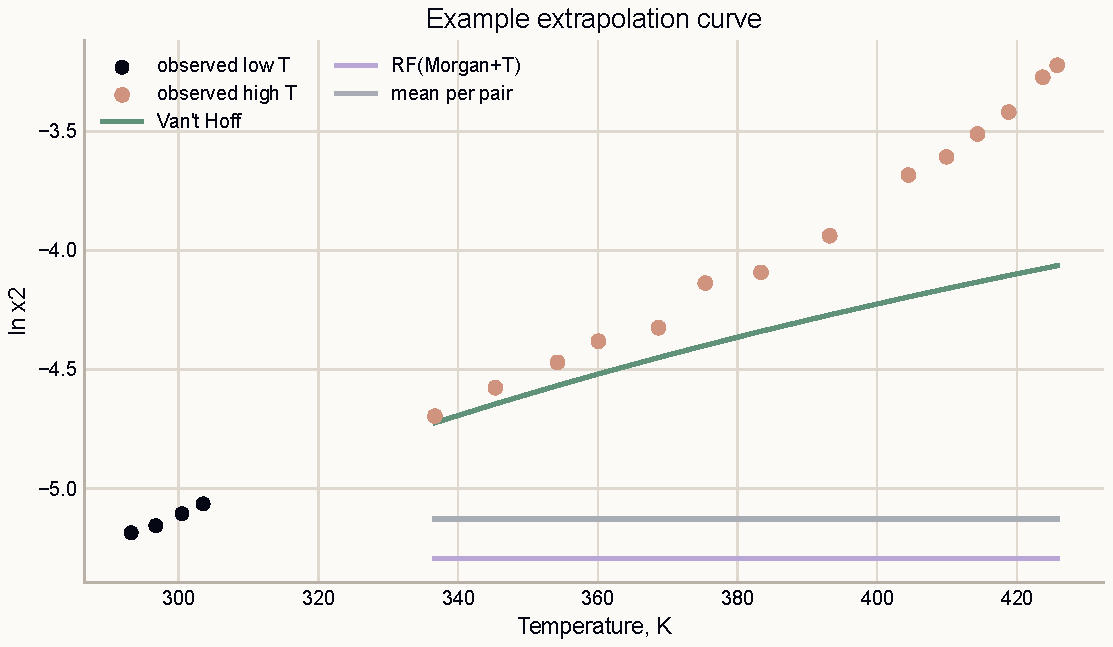
\includegraphics[width=0.88\textwidth]{temperature_extrapolation_example_curves.pdf}
\caption{Типовые температурные кривые для режима одной и той же пары. Низкотемпературные точки задают наклон, а высокотемпературные точки проверяют, сохраняет ли модель физическую форму вне обучающего диапазона.}
\label{fig:temp-extrap-curves}
\end{figure}

Самый важный факт --- Вант-Гофф сильно выигрывает. Это показывает, что температурная физика в данных не является декоративной. Если пара известна и есть несколько температурных точек, простая физическая форма предсказывает высокие температуры намного лучше общих моделей.

Однако это сравнение нужно читать аккуратно. Парная аппроксимация Вант-Гоффа является фактически оракульным ориентиром для известной пары: она подгоняет два параметра отдельно для каждой пары по её низкотемпературным точкам. TGNN-Solv и DirectGNN в текущих кратких запусках получают те же пары в обучающей таблице, но не выполняют отдельной аналитической подгонки параметров для каждой пары при выводе. Поэтому Вант-Гофф здесь не является честным прямым конкурентом модели для прогноза новых пар; он задаёт физический предел, показывающий, какую информацию можно извлечь из температурного ряда пары.

Текущая обучаемая TGNN-Solv этот предел не воспроизводит. Краткий локальный запуск даже хуже DirectGNN. Это говорит не против термодинамики, а против текущей процедуры обучения физической модели: она не восстанавливает парно-специфический температурный наклон с той же эффективностью, с какой это делает явная подгонка Вант-Гоффа.

\subsection{Почему краткий запуск TGNN-Solv не восстанавливает температурную форму}

После аудита протокола был проведён отдельный разбор самих кривых. Для пар, у которых в высокотемпературном тесте есть хотя бы три температурные точки, заново оценивался наклон зависимости $\ln x_2$ от $1/T$:
\[
    \ln x_2 \approx a + b/T.
\]
Затем сравнивался истинный наклон $b$ и наклон, который получается из предсказаний модели на тех же высокотемпературных точках. Такой анализ отделяет два разных вопроса: насколько близко предсказано значение $\ln x_2$ и насколько правильно восстановлена форма температурной кривой.

\begin{table}[H]
\centering
\caption{Восстановление температурного наклона на парах с как минимум тремя высокотемпературными точками.}
\label{tab:temp-slope-diagnostics}
\small
\begin{tabularx}{\textwidth}{Yrrrr}
\toprule
Метод & Пар & MAE по паре & Медианная ошибка наклона, K & Правильный знак \\
\midrule
Вант-Гофф для каждой пары & 389 & 0.425 & 763 & 99.0\% \\
DirectGNN, краткий запуск & 389 & 1.608 & 1 630 & 99.5\% \\
TGNN-Solv, краткий запуск & 389 & 1.894 & 1 158 & 99.7\% \\
Случайный лес с температурой & 389 & 1.280 & 3 386 & 56.0\% \\
\bottomrule
\end{tabularx}
\end{table}

\begin{figure}[H]
\centering
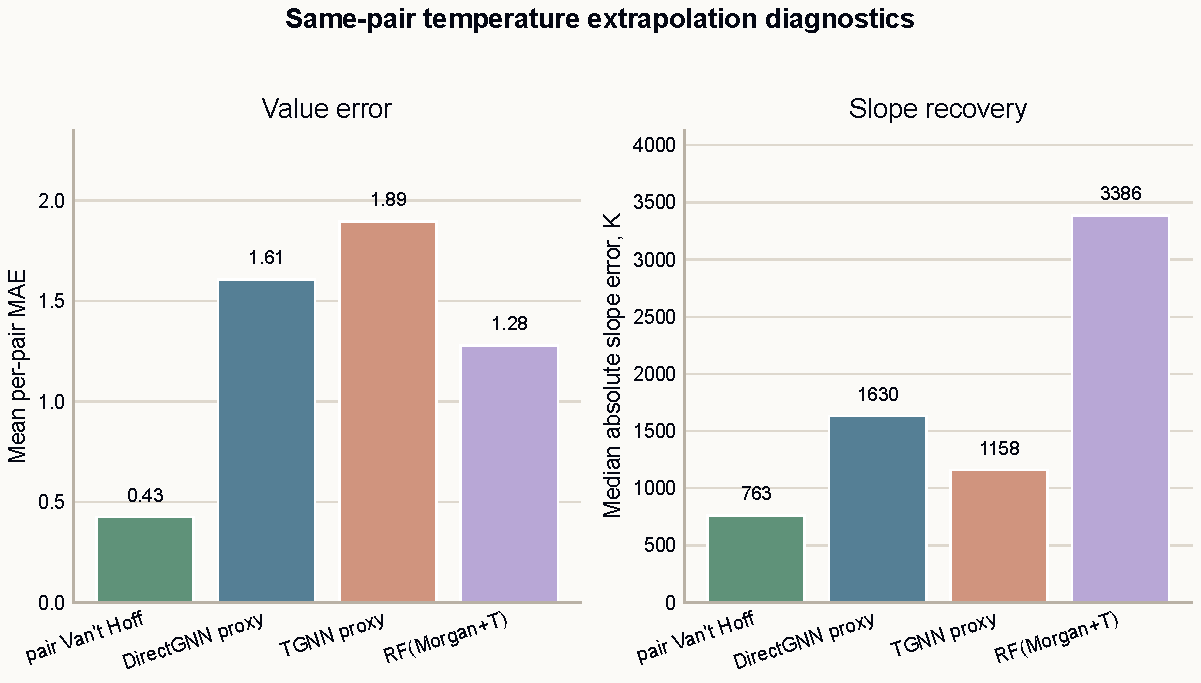
\includegraphics[width=0.94\textwidth]{temperature_slope_recovery_diagnostics.pdf}
\caption{Диагностика значения и наклона на высокотемпературном тесте. TGNN-Solv в кратком запуске лучше DirectGNN по медианной ошибке наклона, но хуже по уровню $\ln x_2$; значит, проблема не сводится к одному знаку температурного тренда.}
\label{fig:temp-slope-diagnostics}
\end{figure}

\begin{figure}[H]
\centering
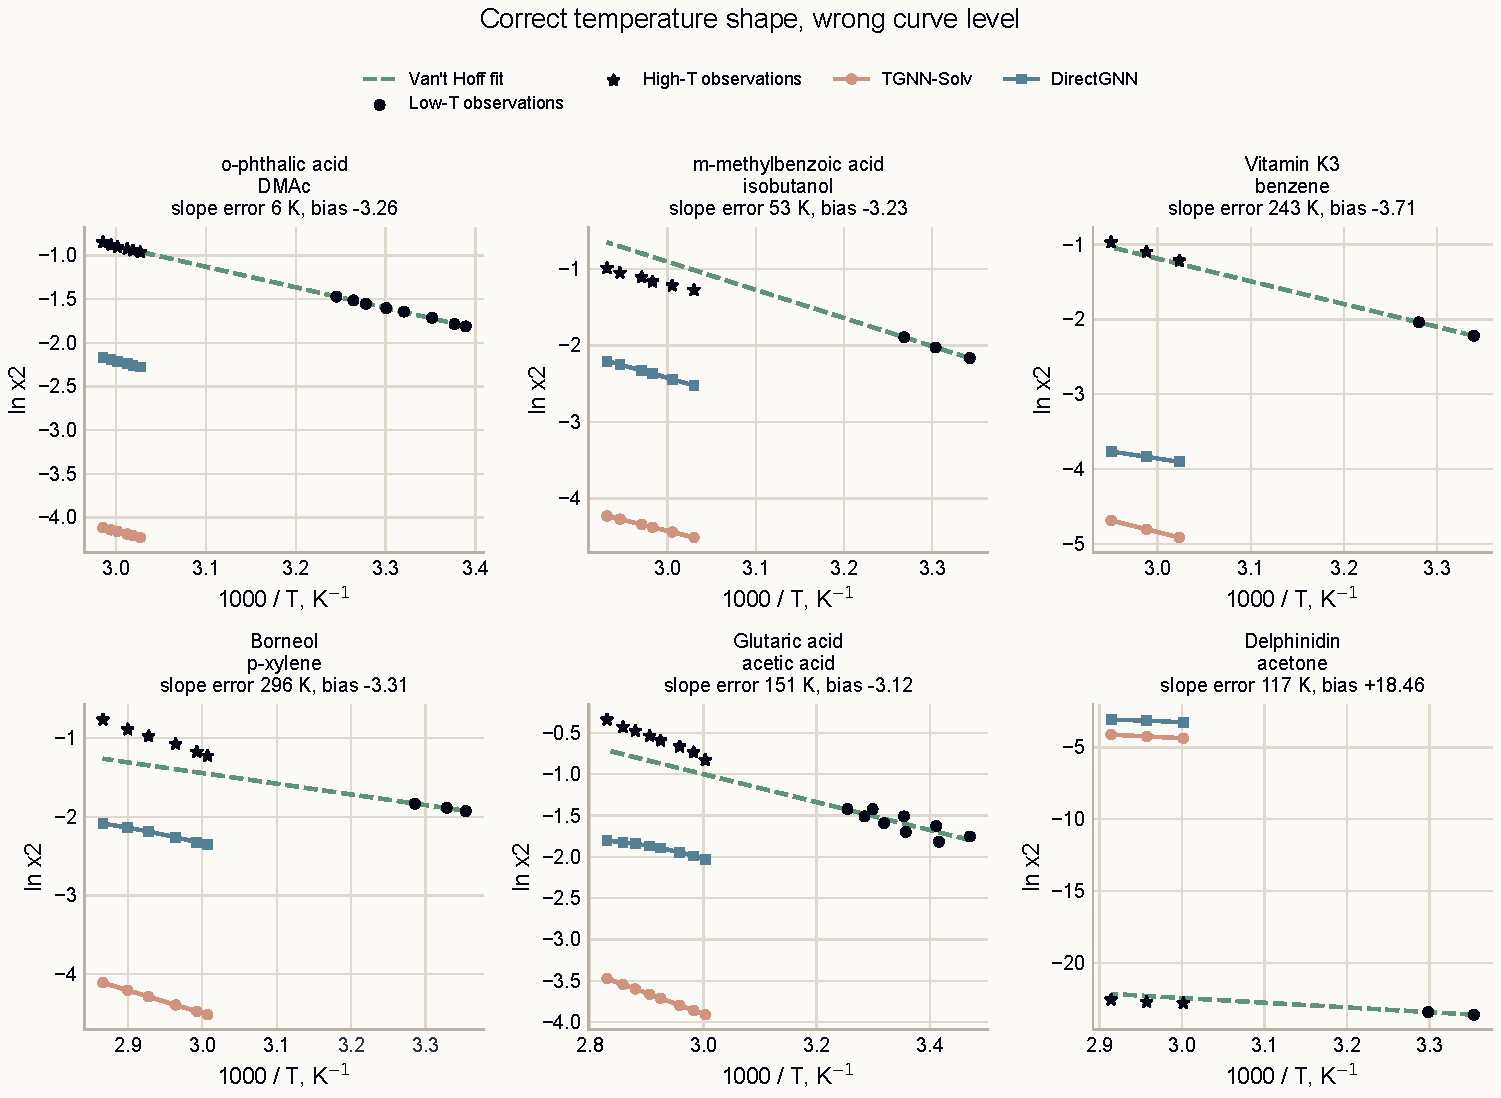
\includegraphics[width=0.96\textwidth]{temperature_slope_level_problem.pdf}
\caption{Пары, на которых TGNN-Solv в кратком запуске относительно неплохо удерживает температурную форму, но промахивается по уровню кривой. Это центральный симптом: модель нередко сохраняет зависимость от температуры, но смещает всю кривую вверх или вниз, потому что вклад активности раствора остаётся слишком слабым.}
\label{fig:temp-slope-level}
\end{figure}

Картина оказалась более конкретной, чем просто «нейросеть не знает температуру». Знак наклона у обеих нейросетевых моделей почти всегда правильный. Но TGNN-Solv в кратком запуске предсказывает слишком однообразные кривые: стандартное отклонение предсказанных наклонов равно примерно $327\,\mathrm{K}$, тогда как у парной аппроксимации Вант-Гоффа оно около $2\,831\,\mathrm{K}$. DirectGNN даёт более широкий набор наклонов, но хуже попадает в их величину. Поэтому следующий температурный эксперимент должен смотреть не только на MAE, но и на распределение наклонов по парам.

Новая галерея на рисунке~\ref{fig:temp-slope-level} делает эту картину зримой. На части пар TGNN-Solv действительно ведёт себя не хаотически: наклон и направление изменения растворимости с температурой улавливаются. Но уровень кривой оказывается систематически смещён. Это согласуется с внутренней диагностикой: кристаллический член $\Phi(T)$ ещё задаёт температурную форму, а ветвь активности раствора почти не вносит парно-специфический вертикальный сдвиг.

Разбор внутренних величин TGNN-Solv показывает причину этого сжатия. В кратком запуске модель почти не использует ветвь активности: $\tau_{12}$ и $\tau_{21}$ имеют стандартное отклонение всего порядка $4.8\cdot 10^{-5}$, а $\ln\gamma_2$ --- порядка $2.9\cdot 10^{-4}$. Практически это означает, что NRTL-часть стала почти константной и не несёт специфики пары. Итоговый прогноз почти полностью определяется кристаллическим членом $\Phi(T)$.

Это ключевое вырождение нужно формулировать прямо. Если $\tau_{12},\tau_{21}$ почти постоянны и $\ln\gamma_2\approx0$ или близок к одному и тому же сдвигу для всех пар, TGNN-Solv перестаёт быть полноценной моделью неидеального раствора и приближается к модели идеальной растворимости:
\begin{equation*}
    \ln x_2 \approx -\Phi(T).
\end{equation*}
В таком режиме правильный наклон может частично сохраняться за счёт кристаллического члена, но уровень кривой ошибается там, где реальный коэффициент активности должен давать большой положительный вклад. Именно поэтому левый хвост плохо растворимых систем оказывается наиболее проблемным. Открытый численный вопрос теперь конкретен: какой минимальный разброс и масштаб $\tau$ достаточны, чтобы физическая ветвь начала улучшать уровень $\ln x_2$, не выходя за допустимые диапазоны параметров.

\begin{figure}[H]
\centering
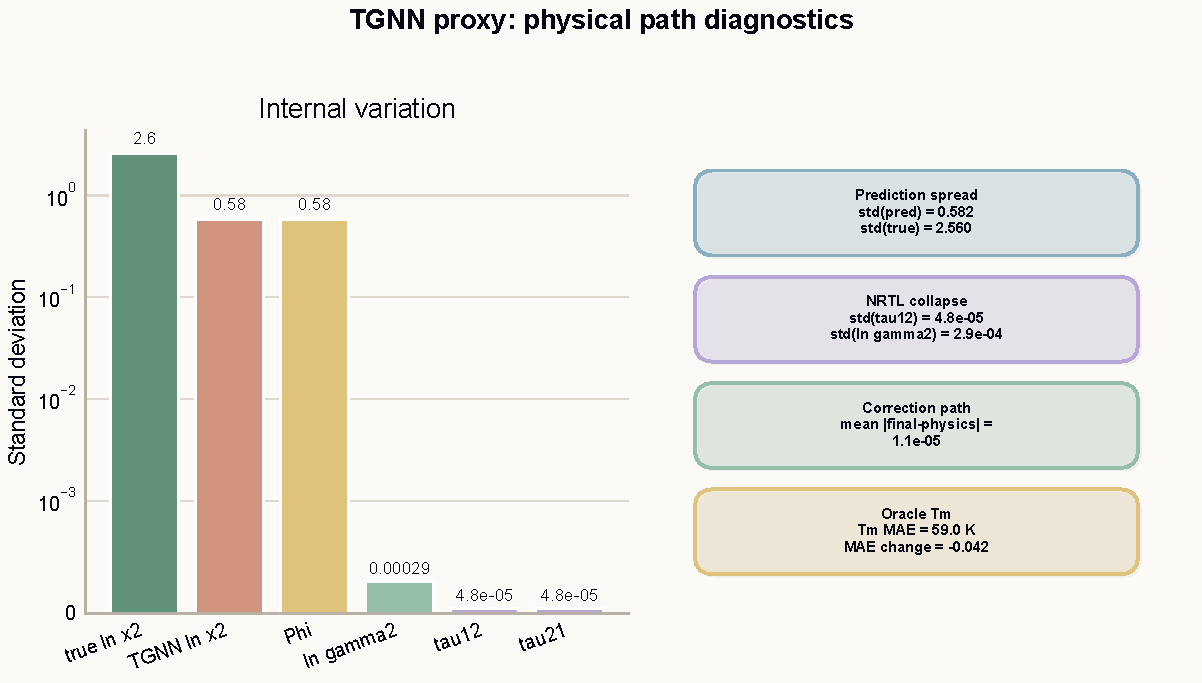
\includegraphics[width=0.94\textwidth]{temperature_tgnn_internal_diagnostics.pdf}
\caption{Внутренние величины TGNN-Solv в кратком температурном запуске. Разброс итоговых предсказаний сильно меньше истинного разброса, NRTL-параметры почти не меняются от пары к паре, а корректирующий путь практически неактивен.}
\label{fig:temp-internal-diagnostics}
\end{figure}

Численно это выглядит так. Истинные значения $\ln x_2$ в высокотемпературной тестовой части имеют стандартное отклонение $2.560$, а предсказания TGNN-Solv --- только $0.582$. Средняя величина поправки между физическим выходом и финальным выходом составляет $1.09\cdot 10^{-5}$, то есть корректирующий путь фактически не меняет ответ. На строках с известной температурой плавления ошибка $\Tm$ равна $59\,\mathrm{K}$, но подстановка истинного $\Tm$ снижает общий MAE только с $1.945$ до $1.903$. Следовательно, в данном кратком запуске проблема не сводится к одному кристаллическому выходному блоку: активность раствора и парная вариативность тоже почти не выучены.

Для проверки, является ли это общей патологией TGNN-Solv или особенностью краткого температурного запуска, те же внутренние величины были сопоставлены со среднебюджетным запуском на каркасном тесте. Картина различается. В кратком температурном запуске NRTL фактически схлопывается: стандартные отклонения $\tau_{12}$ и $\tau_{21}$ составляют около $4.8\cdot 10^{-5}$. В среднебюджетном запуске $\tau$ уже имеет ненулевой разброс и почти всегда остаётся в допустимых пределах. Однако остаточная поправка всё равно почти не улучшает физическое решение. Значит, есть два разных эффекта: в кратком температурном запуске активность почти не выучена вообще, а в более длинном каркасном запуске она выучена слабее, чем нужно для заметного исправления уровня $\ln x_2$.

\begin{figure}[H]
\centering
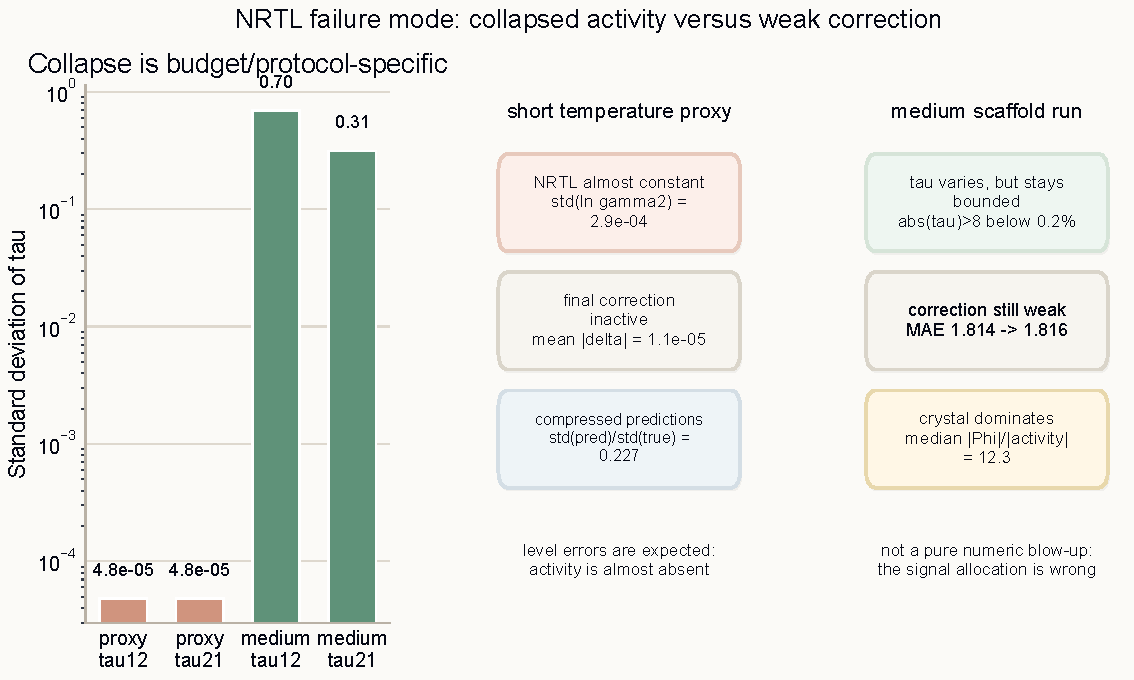
\includegraphics[width=0.92\textwidth]{nrtl_collapse_mechanism.pdf}
\caption{Сравнение двух режимов отказа физического пути. В кратком температурном запуске NRTL-параметры почти константны, поэтому модель сводится к идеальной растворимости с небольшим кристаллическим разбросом. В среднебюджетном каркасном запуске параметры NRTL уже не схлопнуты, но корректирующий путь остаётся слишком слабым и почти не меняет итоговую ошибку.}
\label{fig:nrtl-collapse-mechanism}
\end{figure}

Та же логика проверялась на среднебюджетном запуске TGNN-Solv для каркасного теста. Там остаточная коррекция почти не меняет итог: ошибка физического решения и финального решения практически совпадает. При этом параметры $\tau$ в основном остаются в допустимом диапазоне, то есть проблема не похожа на простой численный взрыв NRTL. Скорее, ветвь активности остаётся слишком слабой относительно кристаллического вклада и получает недостаточно прямого сигнала.

\begin{figure}[H]
\centering
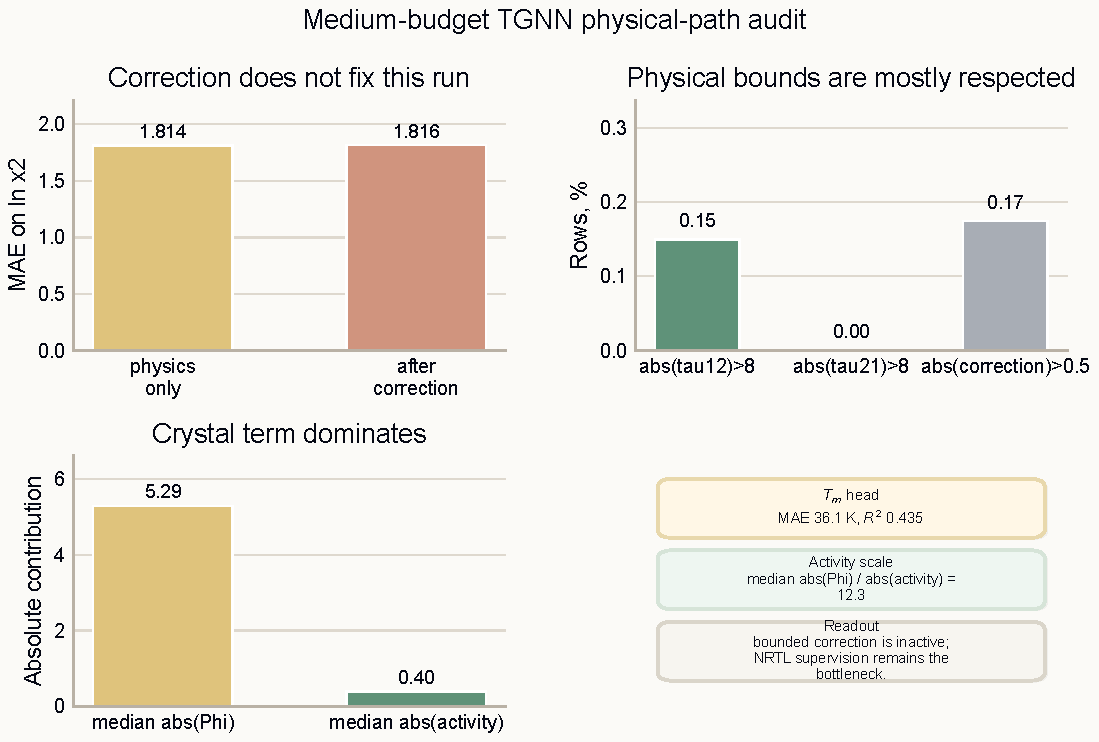
\includegraphics[width=0.92\textwidth]{physics_bottleneck_audit.pdf}
\caption{Аудит физического пути на среднебюджетном запуске TGNN-Solv. Поправочный блок почти не улучшает физическое решение, кристаллический вклад доминирует над активностью, а параметры NRTL в основном находятся в допустимом диапазоне. Это указывает на проблему идентифицируемости и обучающего сигнала, а не на один простой численный сбой.}
\label{fig:physics-bottleneck-audit}
\end{figure}

\begin{table}[H]
\centering
\caption{Химические срезы высокотемпературного теста.}
\label{tab:temp-chemistry-slices}
\begin{tabular}{lrrr}
\toprule
Срез & Вант-Гофф & DirectGNN & TGNN-Solv \\
\midrule
Вода как растворитель & 0.604 & 2.092 & 2.455 \\
Малые растворители, $\le 3$ тяжёлых атома & 0.444 & 1.833 & 2.143 \\
Ароматические растворители & 0.216 & 1.661 & 2.018 \\
Низкая растворимость, $\ln x_2\le -8$ & 0.579 & 4.119 & 5.218 \\
Температура не ниже $360\,\mathrm{K}$ & 1.121 & 1.549 & 1.662 \\
\bottomrule
\end{tabular}
\end{table}

\begin{figure}[H]
\centering
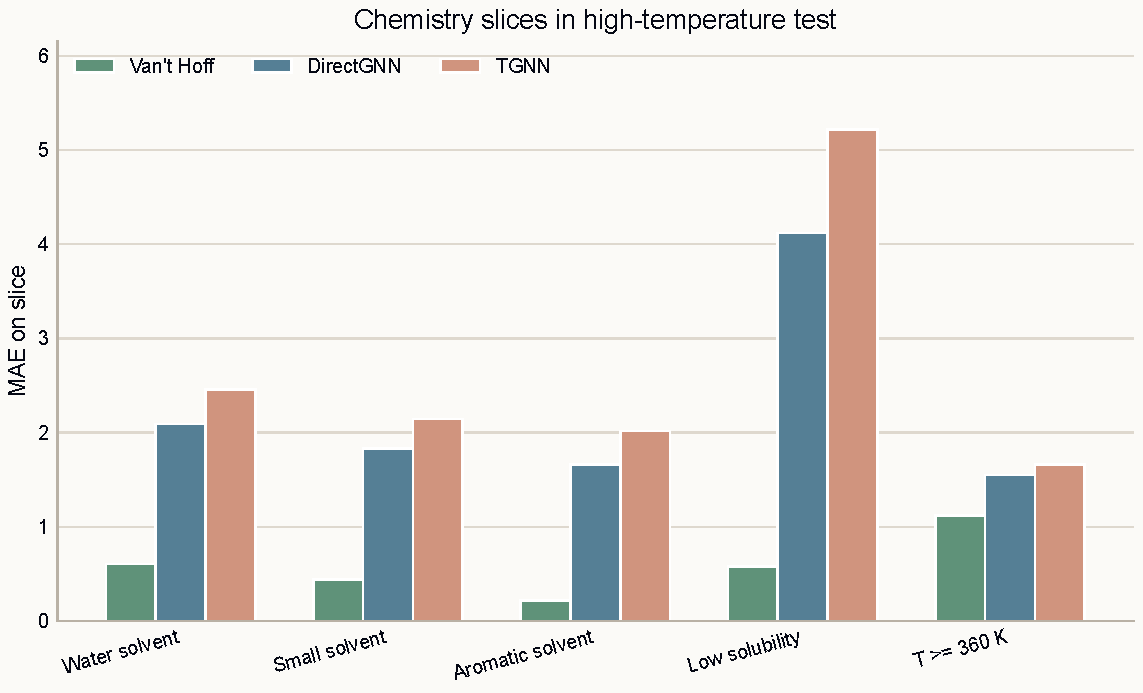
\includegraphics[width=0.92\textwidth]{temperature_chemistry_slice_diagnostics.pdf}
\caption{Срезы температурной экстраполяции по химическим и температурным областям. Вода и малые растворители действительно труднее для нейросетей, но провал TGNN-Solv виден не только на воде; особенно сильна ошибка в области низкой растворимости.}
\label{fig:temp-chemistry-slices}
\end{figure}

Эти срезы уточняют прежнюю гипотезу про воду. Вода ухудшает результат, но не является единственным объяснением: TGNN-Solv также сильно ошибается на малых растворителях, ароматических растворителях и особенно в левом хвосте растворимости. Поэтому исправление графа воды необходимо, но недостаточно. Главная рабочая гипотеза после этой диагностики формулируется строже: в кратком температурном запуске TGNN-Solv не научилась строить парно-различимую активность раствора и поэтому сводит NRTL почти к постоянной поправке.

Отдельно проверены настройки решателя и бюджет этих запусков. В текущем tuned-конфиге используется $5$ итераций решателя при обучении, $20$ при оценке, демпфирование $0.7$, минимальное демпфирование $0.1$ и адаптивное демпфирование. Явной ошибки конфигурации здесь не найдено. Но все нейросетевые числа в этом разделе остаются краткими локальными запусками: DirectGNN обучалась $10$ эпох, TGNN-Solv --- по схеме $1/8/1$, тогда как плановый бюджет обучения равен $50/200/50$. Поэтому эти результаты являются диагностикой механизма отказа, а не окончательным сравнением планового TGNN-Solv с DirectGNN.

\subsection{Интерполяция температуры внутри пары}

Отдельно была проверена более лёгкая задача: у пары есть несколько температур, крайние точки остаются в обучении, внутренние точки удерживаются для проверки. В этом режиме физическая и простая кусочно-линейная интерполяция почти достигают нулевой ошибки.

\begin{table}[H]
\centering
\caption{Интерполяция внутри температурного диапазона пары.}
\label{tab:temp-interp}
\begin{tabular}{lrrr}
\toprule
Метод & $\mae$ & $\Rtwo$ & Правильное направление \\
\midrule
Кусочно-линейная интерполяция & 0.038 & 0.993 & 99.4\% \\
Вант-Гофф для пары & 0.043 & 0.997 & 99.3\% \\
Линейная зависимость от $T$ & 0.045 & 0.997 & 99.3\% \\
Ближайшая температура & 0.195 & 0.986 & 88.8\% \\
Случайный лес с температурой & 0.667 & 0.876 & 95.9\% \\
Среднее по паре & 0.383 & 0.965 & 0.0\% \\
\bottomrule
\end{tabular}
\end{table}

\begin{figure}[H]
\centering
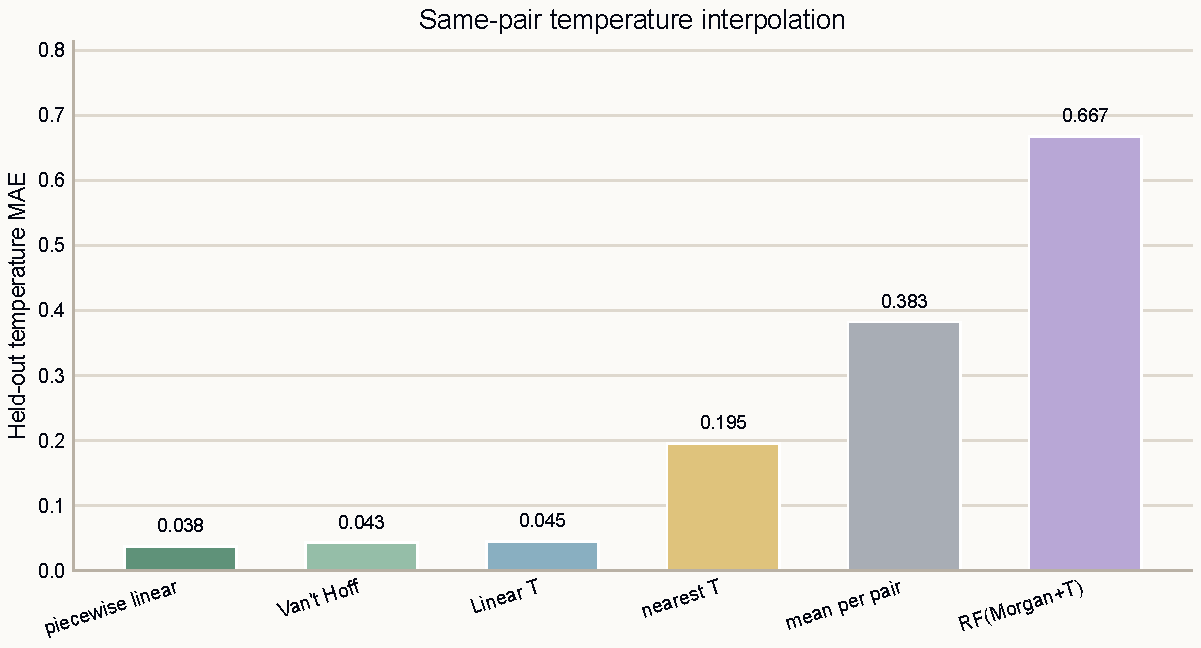
\includegraphics[width=0.88\textwidth]{temperature_interpolation_baseline_comparison.pdf}
\caption{Интерполяция температуры внутри уже известного диапазона пары. Почти нулевая ошибка простых интерполяторов показывает, что повторные температурные измерения в данных физически согласованы.}
\label{fig:temp-interp-bars}
\end{figure}

Эта проверка важна как нижняя граница ошибки. Она показывает, что внутри пары данные очень хорошо согласуются с гладкой температурной кривой. Значит, следующий сильный критерий для TGNN-Solv --- не просто приблизиться к DirectGNN на тесте по новым каркасам, а показать преимущество на переносе низкая температура $\to$ высокая температура для уже известной пары.

\section{Диагностика структурной экстраполяции}

\subsection{Общий вывод}

Структурная экстраполяция трудна для всех проверенных методов. DirectGNN, TGNN-Solv и случайный лес имеют ошибки, сосредоточенные в меньшинстве сложных пар. У DirectGNN медианная ошибка по парам составляет $1.261$, но $17.1\%$ пар имеют $\mae>3.0$.

\subsection{Химические срезы}

На текущем тесте по новым каркасам DirectGNN особенно слаб на галогенированных ароматических веществах: $\mae=1.945$, $\Rtwo=0.380$. Для TGNN-Solv наиболее заметные проигрыши относительно DirectGNN наблюдаются на полиароматических строках и некоторых строках класса «прочее».

\begin{table}[H]
\centering
\caption{Разница ошибки TGNN-Solv минус DirectGNN на отдельных срезах.}
\label{tab:slices}
\begin{tabular}{lr}
\toprule
Срез & Разница MAE \\
\midrule
Полиароматические вещества & $+1.125$ \\
Ароматические растворители & $+0.740$ \\
Кислородсодержащие вещества & $+0.304$ \\
Вода как растворитель & $+0.004$ \\
Углеводородные растворители & $-0.232$ \\
Карбоновые кислоты как растворители & $-0.277$ \\
\bottomrule
\end{tabular}
\end{table}

\begin{figure}[H]
\centering
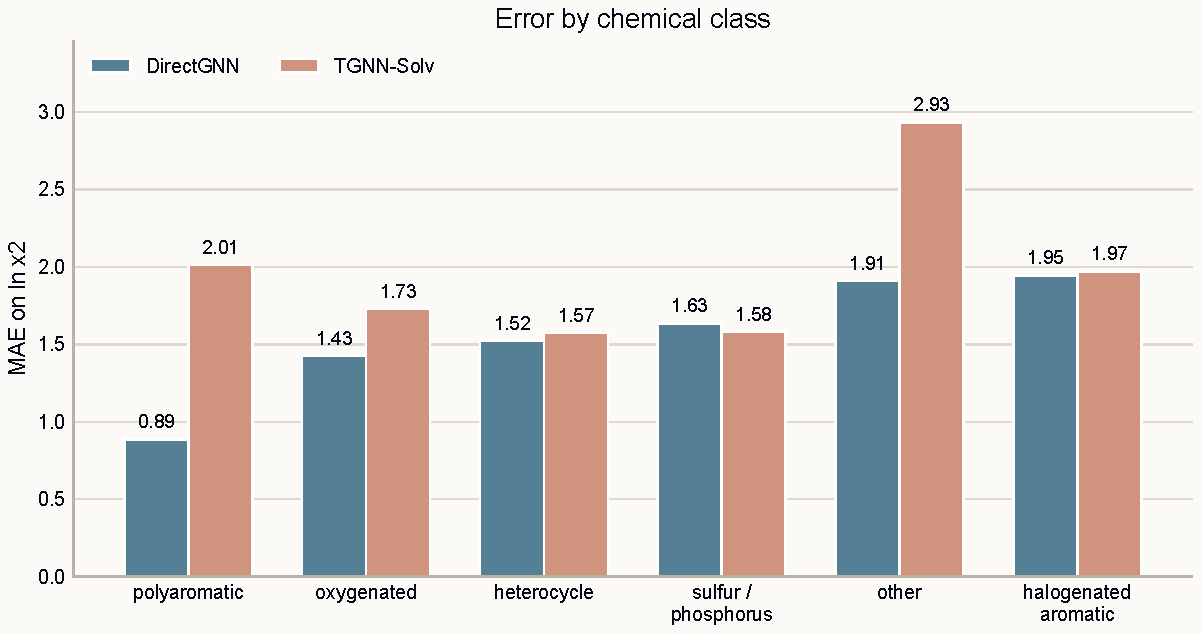
\includegraphics[width=0.88\textwidth]{prediction_slice_chemistry_class_mae.pdf}
\caption{Ошибки по химическим классам. Такие срезы нужны, потому что общий MAE на каркасном разбиении скрывает разные режимы поведения: TGNN-Solv может быть лучше в одних классах и хуже в других.}
\label{fig:chemistry-slices}
\end{figure}

TGNN-Solv не проигрывает одинаково везде. Она теряет качество в одних областях химического пространства и выигрывает в других. Поэтому дальнейшая работа должна оцениваться не только по общей MAE, но и по химическим срезам.

\subsection{Фрагментное покрытие}

Проверка BRICS-фрагментов показала, что тест по новым каркасам не является простой рекомбинацией уже известных фрагментов.

\begin{table}[H]
\centering
\caption{BRICS-покрытие тестовых растворяемых веществ.}
\label{tab:brics}
\begin{tabular}{lrr}
\toprule
Категория & Число & Доля \\
\midrule
Полностью покрыты обучающими фрагментами & 597 & 25.5\% \\
Частично покрыты, больше 50\% фрагментов видны & 690 & 29.5\% \\
Преимущественно новые фрагменты & 1 053 & 45.0\% \\
\bottomrule
\end{tabular}
\end{table}

Фрагментная новизна связана с ошибкой. У DirectGNN MAE на полностью покрытых строках ниже, чем на строках с новыми фрагментами: $1.438$ против $1.717$. У TGNN-Solv разрыв сильнее: $1.385$ против $1.849$. Это обосновывает парное и фрагментное предобучение, но одновременно показывает, что простая фрагментная рекомбинация не решит весь тест по новым каркасам.

\begin{figure}[htbp]
\centering
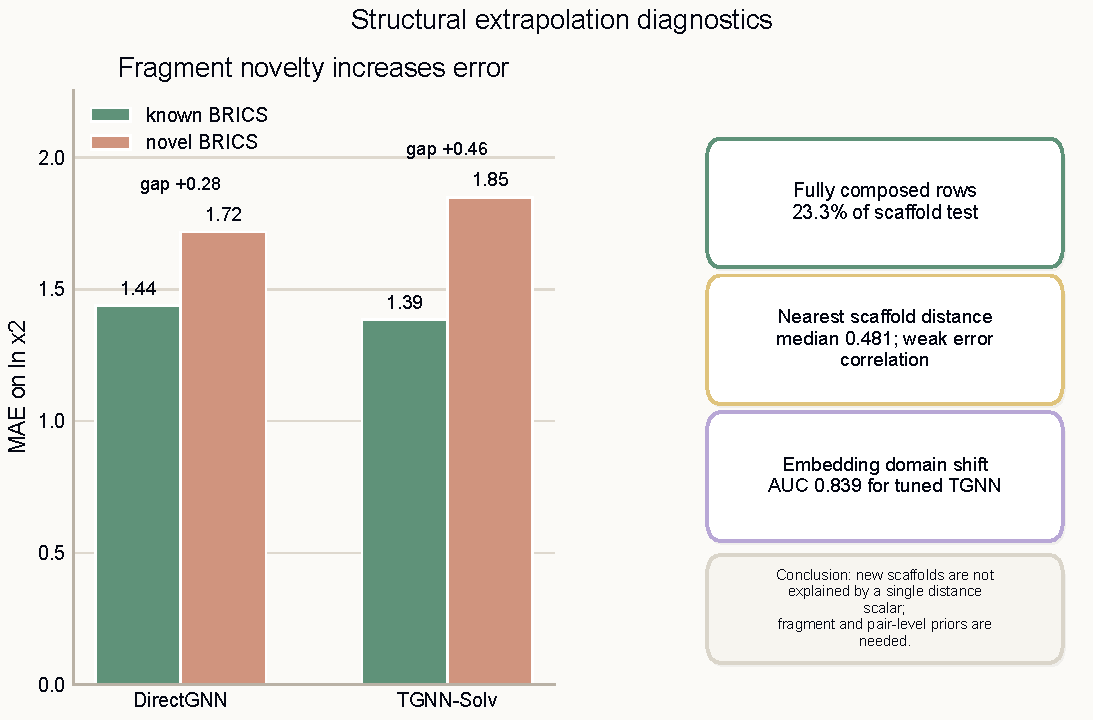
\includegraphics[width=0.92\textwidth]{structural_generalization_diagnostics.pdf}
\caption{Диагностика структурной экстраполяции. Новизна BRICS-фрагментов связана с ростом ошибки, но ближайшее расстояние до обучающего каркаса само по себе слабо объясняет ошибку; значит, нужна не только метрика близости, а переносимые парные и фрагментные представления.}
\label{fig:structural-generalization-diagnostics}
\end{figure}

\subsection{Геометрия химического и скрытого пространства}

Фрагментный анализ показывает только один срез структурной новизны. Поэтому дополнительно построена геометрическая диагностика: сначала в пространстве молекулярных отпечатков Morgan, затем в пространстве векторных представлений, которое выдаёт обученный графовый блок. Такой анализ не является самостоятельной метрикой качества, но отвечает на практический вопрос: видит ли модель тест по новым каркасам как продолжение обучающего пространства или как отдельную область.

\begin{figure}[htbp]
\centering
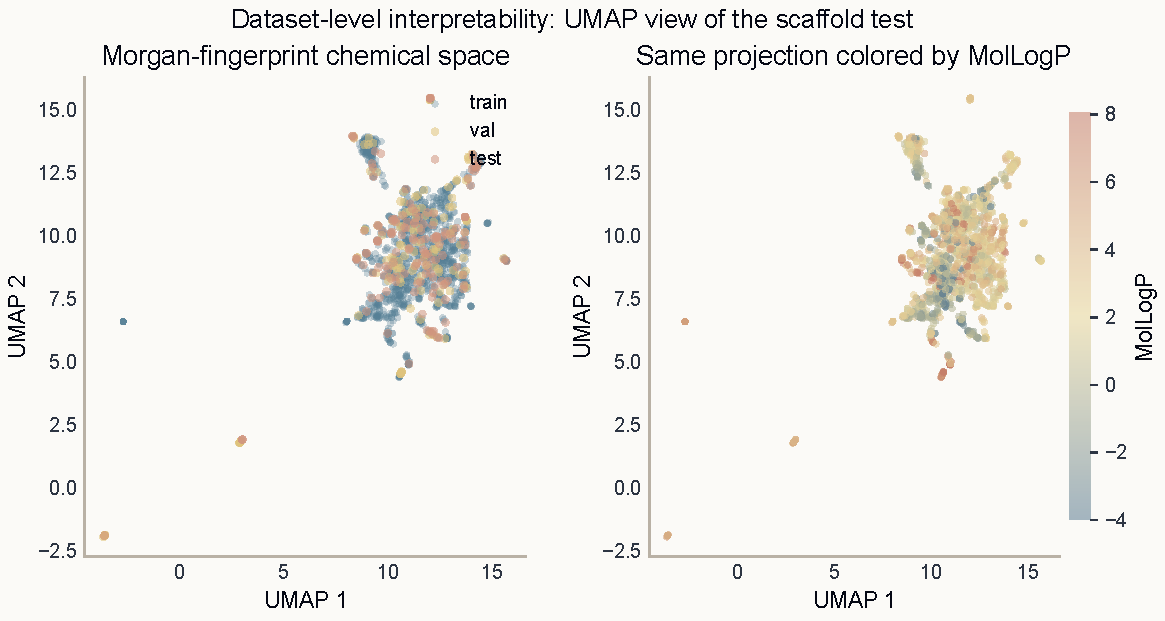
\includegraphics[width=0.88\textwidth]{chemical_space_projection.pdf}
\caption{Проекция химического пространства уникальных растворяемых веществ из SLE-части корпуса. В этой версии используется UMAP-проекция отпечатков Morgan; слева показано положение обучающей, валидационной и тестовой частей, справа та же проекция окрашена по MolLogP.}
\label{fig:chemical-space-projection}
\end{figure}

Проекция по отпечаткам показывает, что тестовые вещества не образуют полностью изолированный остров, но занимают смещённые области того же химического пространства. Это согласуется с результатами по BRICS: задача не сводится ни к простой интерполяции, ни к полностью чужой химии. Для модели это означает, что полезны не только более широкое предобучение одиночных молекул, но и задачи, которые учат совместимость пары вещество--растворитель.

Чтобы эта визуализация была не только иллюстративной, по тем же отпечаткам построена кластеризация на восемь групп. Каждая группа описана через частоты функциональных фрагментов и через ошибки моделей на строках, где растворяемое вещество попадает в эту группу. Получившаяся картина полезна тем, что показывает не только «где находятся» новые каркасы, но и где физический путь действительно помогает. Например, TGNN-Solv оказывается лучше DirectGNN в небольшой гидрофобной группе с длинными алкильными фрагментами, но заметно хуже в группе гидроксильных и карбонильных соединений. Это уже не глобальная метрика, а диагностическая карта химических режимов.

\begin{figure}[htbp]
\centering
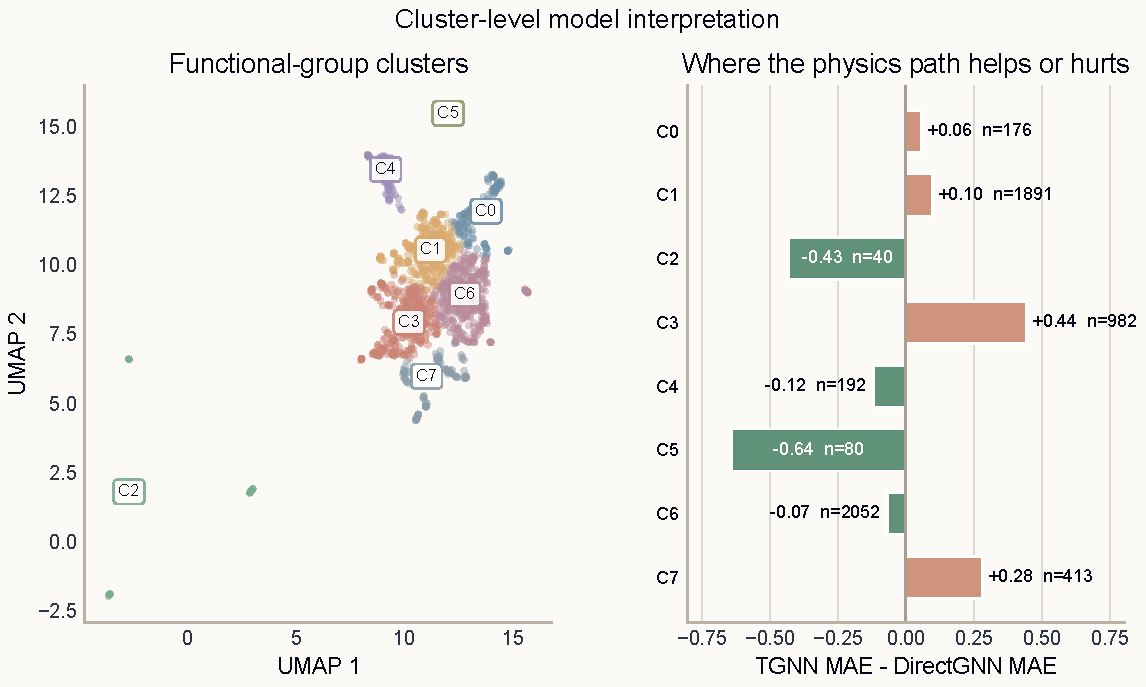
\includegraphics[width=0.90\textwidth]{cluster_error_interpretability.pdf}
\caption{Кластерная интерпретация химического пространства. Слева показаны группы веществ в UMAP-пространстве отпечатков Morgan; справа --- разница ошибок TGNN-Solv и DirectGNN по тем же группам. Отрицательное значение означает преимущество физической модели, положительное --- проигрыш относительно прямой нейросетевой модели.}
\label{fig:cluster-error-interpretability}
\end{figure}

\begin{figure}[htbp]
\centering
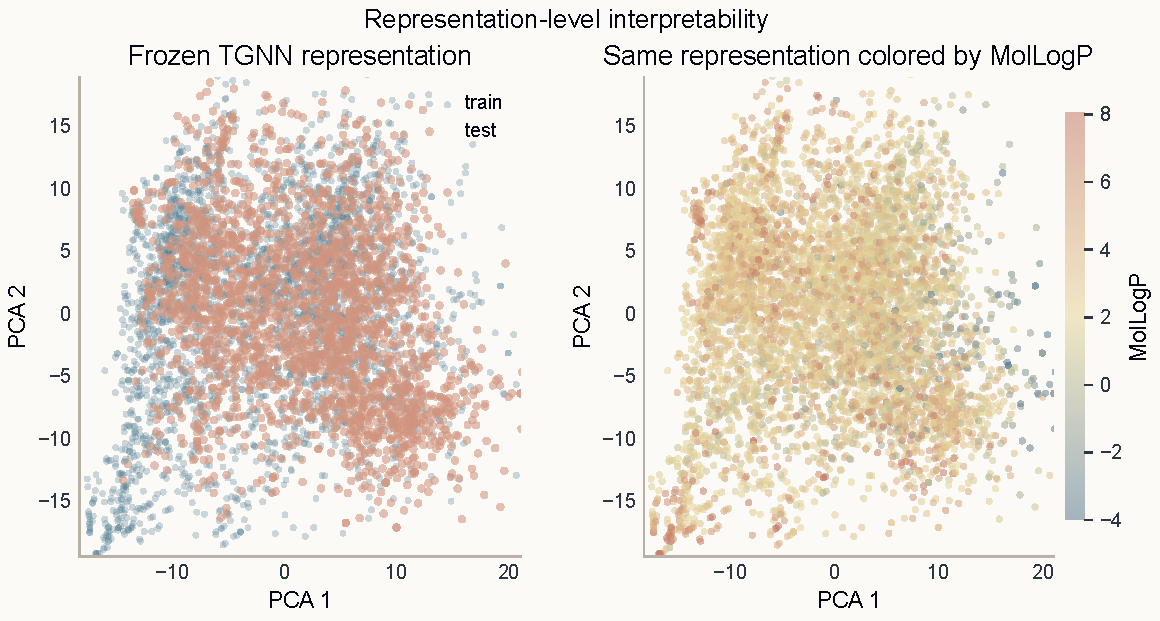
\includegraphics[width=0.88\textwidth]{embedding_geometry_diagnostics.pdf}
\caption{Геометрия скрытых представлений TGNN-Solv после обучения. Здесь использована устойчивая PCA-проекция сохранённых 768-мерных представлений; она показывает, что обучающая и тестовая части не полностью перемешиваются в пространстве признаков.}
\label{fig:embedding-geometry-diagnostics}
\end{figure}

Этот результат важен для интерпретируемости. Если бы обученные представления полностью перемешивали обучающую и тестовую части, основная ошибка была бы скорее следствием выходных блоков или физического решателя. Здесь же сдвиг виден ещё до выхода модели. Поэтому гипотеза о парном и фрагментном предобучении остаётся содержательной: нужно не только точнее решать SLE, но и строить такое представление, где новые каркасы описываются через переносимые химические признаки.

\section{Расширение физического обучающего сигнала}

\subsection{IDAC}

Одна из главных проблем TGNN-Solv --- слабый прямой обучающий сигнал для параметров активности; поэтому особенно важны внешние термодинамические архивы и стандартизованные форматы данных~\cite{frenkel2006,nist_thermoml,ddb2024}. В исходной версии было только $404$ строки IDAC, $138$ уникальных пар и $9$ DOI. После расширения через NIST ThermoML получено $14\,900$ агрегированных строк, $3\,145$ уникальных пар и $63$ DOI.

\begin{table}[H]
\centering
\caption{Расширение IDAC-данных.}
\begin{tabular}{lrr}
\toprule
Показатель & Старый набор & Расширенный набор \\
\midrule
Строки & 404 & 14 900 \\
Уникальные пары & 138 & 3 145 \\
DOI & 9 & 63 \\
Конфликтующие группы при $\mathrm{std}>0.5$ & --- & 0 \\
Пересечение с SLE-парами & --- & 0\% \\
\bottomrule
\end{tabular}
\end{table}

IDAC не добавляется как строка растворимости. Это другая физическая величина, связанная с теми же параметрами активности, поэтому она подключена отдельным вспомогательным потоком. Схема извлечения, агрегирования и проверки этого корпуса приведена выше в разделе данных.

\subsection{UNIFAC}

Установлены и подключены пакеты \code{thermo}, \code{chemicals} и \code{lxml}, что позволило использовать расчёты Modified UNIFAC~\cite{fredenslund1975,weidlich1987}. На их основе подготовлен дополнительный поток псевдометок для $\ln\gamma_2^\infty$. Он содержит $39\,459$ строк, из которых $14\,900$ --- экспериментальные IDAC-строки, а $24\,559$ --- псевдометки UNIFAC. Псевдометки имеют меньший вес: $0.15$ против $1.0$ у экспериментальных строк.

Покрытие UNIFAC-приоров на основном тесте по новым каркасам ограничено: около $8.6\%$ строк и $10.9\%$ уникальных пар. Поэтому UNIFAC не может быть единственным решением структурной экстраполяции, но может служить физическим приором там, где группы распознаны.

\section{Актуальные рабочие гипотезы}

Текущий проектный статус лучше описывать не как набор несвязанных улучшений, а как проверку нескольких конкретных гипотез. Часть из них уже подтверждена диагностически, часть остаётся рабочей и требует полного вычислительного бюджета.

\begin{figure}[H]
\centering
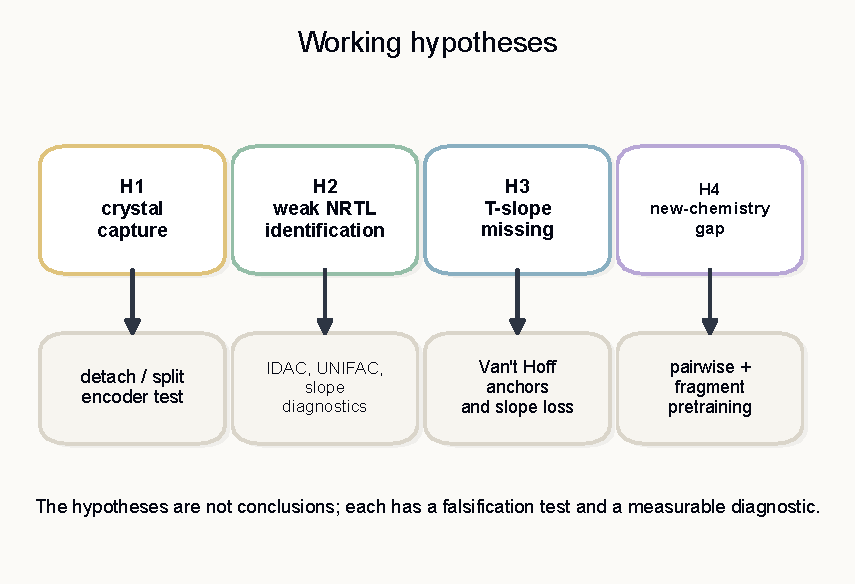
\includegraphics[width=0.94\textwidth]{hypothesis_map_schematic.pdf}
\caption{Карта текущих рабочих гипотез. Каждая гипотеза связана не с общим рассуждением, а с конкретным проверяемым экспериментом или диагностикой.}
\label{fig:hypothesis-map}
\end{figure}

\textbf{Гипотеза 1: кристаллическая ветвь перетягивает представление.}
У $T_m$ есть гораздо больше прямых меток, чем у параметров активности. Поэтому общий графовый блок может учиться в первую очередь признакам чистого твёрдого вещества: массе, жёсткости, симметрии и упаковке. Эти признаки полезны для плавления, но не полностью совпадают с признаками жидкофазной совместимости. Проверка этой гипотезы --- режимы раздельных адаптеров, частичное отключение кристаллического градиента во второй фазе и сравнение с вспомогательной прямой ошибкой по растворимости для парной ветви.

\textbf{Гипотеза 2: NRTL-параметры плохо идентифицируются из одной SLE-метки.}
Параметры $\tau_{12}$, $\tau_{21}$ и $\alpha$ не измеряются напрямую. Одна точка растворимости задаёт только одно скалярное условие, а разные наборы параметров могут давать почти одинаковый $\ln x_2$. Поэтому расширение IDAC, UNIFAC-псевдометки, ограничения диапазонов $\tau$ и диагностический анализ распределений NRTL-параметров являются не дополнительными украшениями, а способом сделать обратную задачу лучше обусловленной.

\textbf{Гипотеза 3: температурный наклон и уровень кривой разделяются плохо.}
Аппроксимация Вант-Гоффа показывает, что внутри одной пары температурная форма очень информативна: ошибка $0.368$ на высокотемпературной экстраполяции достижима без сложной нейросети. Дополнительный аудит подтвердил, что это именно режим известной пары: пересечение низкотемпературной обучающей и высокотемпературной тестовой частями по парам равно $100\%$, а положительный сдвиг растворимости наблюдается у $99.6\%$ пар. Новый анализ наклонов уточнил проблему: TGNN-Solv в кратком запуске почти всегда даёт правильный знак наклона и имеет меньшую медианную ошибку наклона, чем DirectGNN, но при этом хуже по уровню $\ln x_2$. Внутренние величины показывают, что NRTL-ветвь почти схлопнулась к константе. Следовательно, следующий эксперимент должен одновременно контролировать наклон, уровень кривой и вариативность параметров активности.

\textbf{Гипотеза 4: одиночного молекулярного предобучения недостаточно для структурной экстраполяции.}
ZINC250k и другие широкие наборы помогают графовому блоку узнать химию одиночных молекул. Но растворимость является парным свойством: нужна совместимость вещества и растворителя. Поэтому подготовлены парные контрастивные задачи, анализ фрагментного покрытия и статистика «обрывов растворимости», где структурно близкие вещества резко отличаются по растворимости в одном растворителе.

\textbf{Гипотеза 5: часть физической ошибки систематична, а не статистична.}
Приближение $\Delta C_p^{\mathrm{fus}}=0$ может давать вклад порядка $0.5$--$0.8$ в $\ln x_2$; одноатомный граф воды теряет O--H-связи; мостовой компонент теории регулярных растворов может вредить водородно-связанным системам. Эти случаи не исправляются простым увеличением числа эпох. Для них нужны отдельные физические или представленные исправления, часть которых уже реализована.

\section{Проверенные отрицательные результаты}

Отрицательные результаты важны, потому что сужают пространство объяснений.

\subsection{Преобразование единиц}

Аудит переходов между $\ln x_2$ и $\log S$ показал, что средняя ошибка обратного преобразования в обработанных разбиениях находится около машинной точности. В сыром корпусе среднее расхождение между доступными $x_2$ и $\log S$ соответствует примерно $0.014$ в $\ln x_2$, что на два порядка меньше текущих ошибок моделей. Следовательно, основная ошибка порядка $1.6$ по MAE не объясняется преобразованием единиц.

\subsection{Левый хвост распределения}

Тестовое разбиение по новым каркасам действительно смещено к более низкой растворимости и более тяжёлым каркасам. Однако удаление экстремального хвоста $\ln x_2<-15$ улучшает $\Rtwo$ только примерно на $0.01$--$0.02$. Значит, хвост важен, но не является единственной причиной низкого качества.

\subsection{Взвешивание источников}

Первый механизм весов по предполагаемой надёжности источника на малом согласованном подмножестве ухудшил DirectGNN: MAE выросла с $2.120$ до $2.331$. Для TGNN-Solv изменение было малым, но тоже отрицательным: $2.393$ против $2.412$. Инфраструктура для учёта источников полезна, но текущие эвристические веса не являются готовым улучшением.

\begin{figure}[H]
\centering
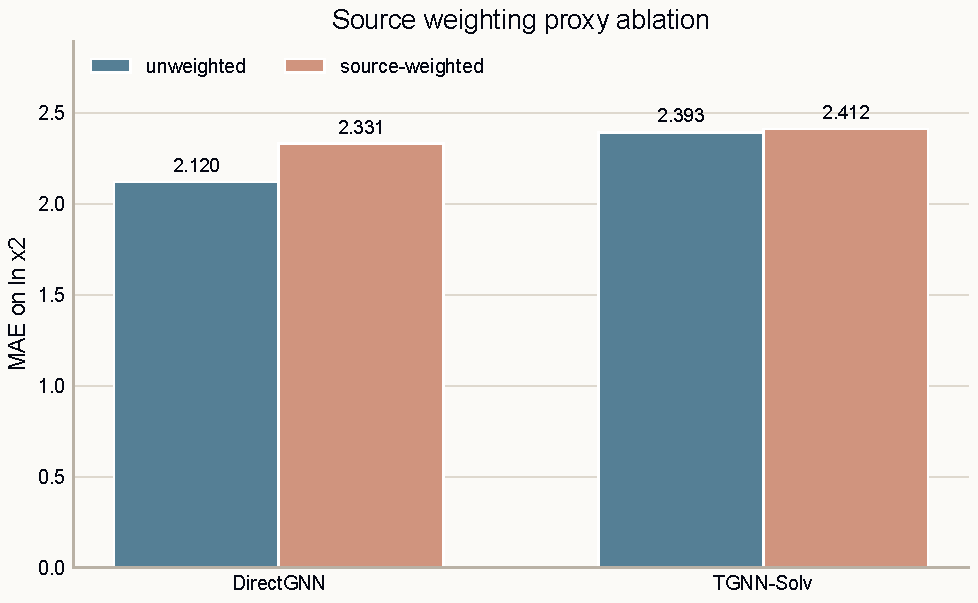
\includegraphics[width=0.82\textwidth]{source_weighting_ablation.pdf}
\caption{Проверка первого варианта весов по источникам на согласованном подмножестве. Взвешивание источников не улучшило качество и потому не используется как основной результат; оно оставлено как диагностическая инфраструктура для будущих более строгих оценок неопределённости источника.}
\label{fig:source-weighting-ablation}
\end{figure}

\subsection{Простое усиление температурных ограничений}

Краткие локальные проверки улучшенной TGNN-Solv на температурной экстраполяции не решили задачу. Лучший из таких запусков имел $\mae=1.986$, что всё ещё хуже старого краткого запуска TGNN-Solv $1.945$ и DirectGNN $1.619$. Это означает, что добавленные компоненты нужно проверять на плановом бюджете и с более прямой постановкой температурной функции обучения.

\section{Интерпретация, неопределённость и прикладной слой}

\subsection{Что говорят данные о моделируемости}

Отдельная проверка была проведена для вопроса, не является ли корпус в принципе слишком шумным или хаотичным. Простая модель ближайшего соседа по сходству по коэффициенту Танимото пары даёт на полном разбиении $\mae=2.530$, то есть заметно хуже случайного леса ($1.722$) и DirectGNN ($1.652$). Значит, задача не сводится к грубому поиску ближайшей известной пары; обучаемые модели действительно извлекают переносимые закономерности.

При этом локальные «обрывы растворимости» существуют. Даже структурно похожие вещества могут резко отличаться по растворимости в одном растворителе. Поэтому корректный вывод двойной: корпус моделируем, но структурная экстраполяция остаётся трудной. Это согласуется с наблюдением, что на близких парах TGNN-Solv иногда выигрывает, а на средних химических расстояниях ошибки физического пути могут усиливаться через параметры NRTL.

\subsection{Карты вклада атомов}

Интерпретационный слой в проекте используется не как доказательство правильности модели, а как контроль здравого смысла. Для отдельных прогнозов строятся карты вклада атомов: какие части молекулы сильнее всего влияют на итоговую растворимость или на промежуточные физические величины. Это особенно полезно при сравнении обычного MPNN и TIMP-кодировщика: во втором случае вклад можно сопоставлять не только с итоговым числом, но и с дисперсионным и полярным каналами.

\begin{figure}[H]
\centering
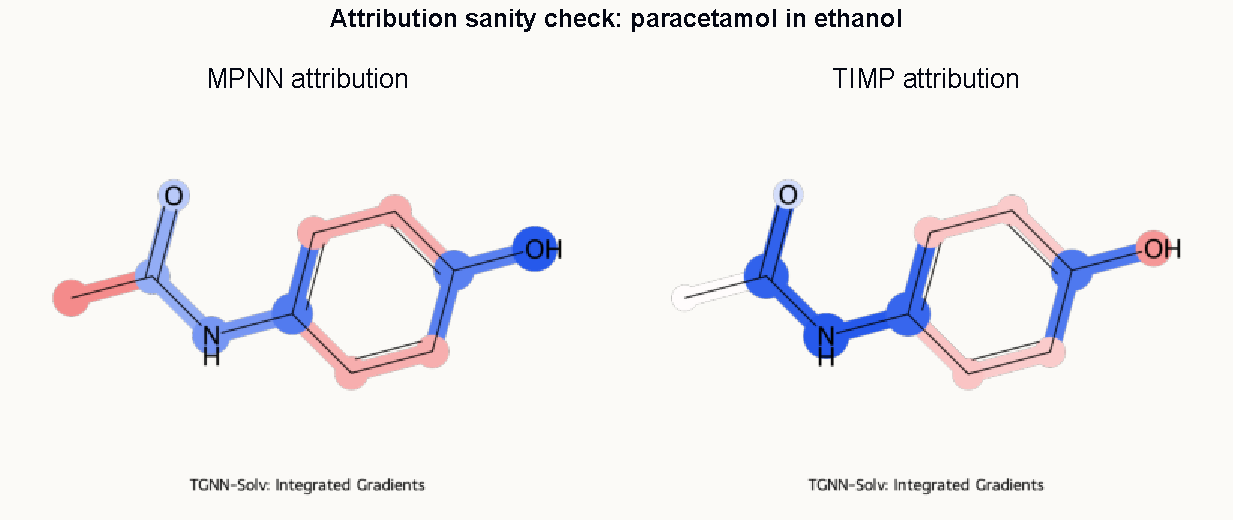
\includegraphics[width=0.92\textwidth]{attribution_examples.pdf}
\caption{Пример интерпретационных карт для пары парацетамол--этанол. Цель таких рисунков --- не заменить физическую проверку, а увидеть, концентрируется ли модель на химически ожидаемых областях: гетероатомах, донорно-акцепторных центрах и полярных фрагментах.}
\label{fig:attribution-examples}
\end{figure}

Такие карты также помогают находить ошибки постановки. Если вклад систематически концентрируется на нерелевантных атомах или исчезает в полярном канале для водных систем, это сигнал к проверке графовой топологии, признаков связей и супервизии каналов. Именно поэтому в TIMP-экспериментах были добавлены отдельные диагностические тесты на разделение дисперсионного и полярного каналов.

\subsection{Неопределённость и область применимости}

Для практического использования одного числа $\widehat{\ln x_2}$ недостаточно. Пользователь должен понимать, находится ли запрос рядом с обучающей областью и насколько широким должен быть доверительный интервал прогноза. Поэтому в проекте реализованы слой неопределённости и диагностика области применимости. Неопределённость может оцениваться через метод Монте-Карло со случайным выключением нейронов или ансамбль моделей~\cite{gal2016,lakshminarayanan2017}; калибровка интервалов рассматривается отдельно, потому что низкая дисперсия предсказаний не гарантирует малую ошибку~\cite{guo2017}.

На текущем этапе это реализованный прикладной контур, а не завершённый результат калибровки. Для финальной отчётности здесь должны появиться числа $\mathrm{PICP}_{90}$, средняя ширина интервала и зависимость ошибки от расстояния до обучающей области. В имеющихся артефактах есть только малые лабораторные прогоны калибровки, поэтому они не используются как показатель качества модели на основном каркасном тесте.

Область применимости строится по двум типам расстояний. Первый --- расстояние в пространстве скрытых представлений пары, где модель фактически делает прогноз. Второй --- химическое сходство отпечатков Моргана по коэффициенту Танимото для растворяемого вещества и растворителя~\cite{rogers2010}. Такая комбинация нужна, потому что расстояние в пространстве скрытых представлений учитывает обученную задачу, а коэффициент Танимото даёт химически понятный контроль: видел ли корпус похожие структуры.

\begin{figure}[H]
\centering
\includegraphics[width=0.90\textwidth]{uncertainty_ad_schematic.pdf}
\caption{Слой неопределённости и области применимости не меняет физическую модель, а сопровождает прогноз интервалом, флагом выхода из обучающей области и химически понятными расстояниями до известных примеров.}
\label{fig:uncertainty-ad}
\end{figure}

\subsection{Реализованные прикладные сценарии}

Поверх обученной модели подготовлены прикладные сценарии: быстрый прогноз для одной пары, температурное сканирование, ранжирование растворителей, подбор технологического окна, предварительная оценка растворимости лекарственных молекул и профиль растворимости для фармакокинетических расчётов. Эти модули не являются отдельными научными результатами отчёта, но они важны как проверка инженерной завершённости: одна и та же модель используется не только в таблице метрик, но и в воспроизводимых рабочих сценариях.

Прикладной слой специально отделён от научного сравнения TGNN-Solv и DirectGNN. В отчёт не выносится пользовательская документация интерфейса, но фиксируется, что модель уже поддерживает применение модели к новой паре, интерпретационный вывод, температурные кривые, отчёт о физических промежуточных величинах и проверку области применимости.

Отдельный практический показатель ещё не закрыт: время одного предсказания и отношение скорости TGNN-Solv к DirectGNN. Из-за итеративного SLE-решателя TGNN-Solv заведомо дороже прямой модели, но для скрининга важна не только относительная, а абсолютная задержка на пару и на температурную сетку. Поэтому в следующем пакете отчётности нужно небольшое измерение времени вывода на CPU и GPU с одинаковым мини-пакетом.


\section{Подготовленные проверки и оставшаяся неопределённость}

В проекте уже выполнена не только реализация основной модели, но и значительная часть проверочной инфраструктуры. Ниже эта работа сведена не как технический перечень файлов, а как научная карта того, что именно теперь можно проверять.

\begin{table}[H]
\centering
\caption{Основные блоки проделанной работы и их текущий статус.}
\label{tab:implemented-work}
\small
\begin{tabularx}{\textwidth}{P{0.22\textwidth}Y P{0.18\textwidth}}
\toprule
Направление & Что сделано & Статус \\
\midrule
Данные & Подготовлены обработанные разбиения BigSolDB v2.1, проверены дубликаты, сохранены водные системы, добавлены температурные разбиения & готово \\
Физическая модель & Реализованы SLE-решатель, NRTL, IDAC-предел, теплоёмкостная формула и диагностические промежуточные выходы & готово \\
Контрольные модели & Реализованы DirectGNN, случайный лес и внешние сравнения с SolProp и FastSolv & готово \\
Обучение & Поддержаны этап 0, трёхфазная схема, маски вспомогательных меток, отдельный IDAC-поток и оракульные проверки & готово \\
Устранение слабых мест & Добавлены явные водороды для малых молекул, энтропийно согласованная кристаллическая ветвь, UNIFAC-псевдометки и парные задачи & частично проверено \\
Диагностика & Выполнены split hierarchy, аудит температурного протокола, анализ наклонов Вант-Гоффа, внутренние величины TGNN-Solv, температурные химические срезы, интерполяция, BRICS-анализ и анализ воды & готово \\
Полные проверки & Многосидовые запуски планового бюджета и абляции новых компонентов & требуют GPU \\
\bottomrule
\end{tabularx}
\end{table}

Критически важно, что не все реализованные блоки уже доказали пользу в финальном режиме. Таблица~\ref{tab:ablation-status} поэтому не выдаёт малые отладочные прогоны за полноценные результаты, а показывает текущий статус доказательности.

\begin{table}[H]
\centering
\caption{Статус абляций основных архитектурных и обучающих компонентов.}
\label{tab:ablation-status}
\small
\begin{tabularx}{\textwidth}{P{0.25\textwidth}P{0.24\textwidth}Y}
\toprule
Компонент & Что есть сейчас & Что можно утверждать \\
\midrule
TIMP-кодировщик & краткое диагностическое сравнение: TGNN-TIMP $\mae=1.847$, TIMP+Hansen contrastive $\mae=1.820$ против TGNN-MPNN $\mae=1.741$ & каналы и представления диагностически полезны, но финального выигрыша MAE нет \\
Контрастивное выравнивание Хансена & улучшает краткий TIMP-прогон относительно TIMP без него, но остаётся хуже MPNN & это метрическое выравнивание представлений, а не доказательство физической чистоты каналов \\
Вспомогательный IDAC-поток & есть отдельный поток и малый CPU-прогон; полноразмерной абляции нет & перенос с IDAC-пар на SLE-пары остаётся проверяемым допущением \\
UNIFAC-псевдометки & есть покрытие train/test и подключение как слабого сигнала & покрытие scaffold-test низкое ($8.6\%$ строк), standalone MAE ещё не посчитан \\
Явные водороды для воды и малых молекул & реализованы и проверены графовые контракты & необходимая инженерная правка, но не доказанный источник общего MAE-выигрыша \\
Энтропийная кристаллическая параметризация & реализована в конфигурациях и описана математически & требует одинакового сравнения на плановом бюджете с независимыми $\Tm,\dHfus$-головами \\
MoE по типам растворителей & реализована маршрутизация и баланс экспертов & вклад в качество не установлен без отдельной абляции \\
\bottomrule
\end{tabularx}
\end{table}

Для следующего вычислительного этапа важно заранее зафиксировать, какие результаты будут считаться содержательными. Иначе есть риск снова получить отдельный MAE без понимания, какой именно механизм изменился.

\begin{table}[H]
\centering
\caption{Минимальный набор проверок для полноразмерного следующего этапа.}
\label{tab:next-validation-contract}
\small
\begin{tabularx}{\textwidth}{P{0.26\textwidth}Y P{0.25\textwidth}}
\toprule
Проверка & Что измеряет & Критерий полезности \\
\midrule
Температурная экстраполяция, плановый бюджет & Использует ли TGNN-Solv известную форму зависимости от температуры & MAE ниже DirectGNN и заметное улучшение наклона Вант-Гоффа \\
Контрольная подстановка кристалла & Какая часть ошибки идёт от $T_m$ и $\Delta H_{\mathrm{fus}}$ & Существенная разница между полной моделью и режимом с известными кристаллическими параметрами локализует кристаллическую ошибку \\
Аудит NRTL-параметров & Стали ли $\tau_{12},\tau_{21},\alpha$ парно-различимыми и физически ограниченными & Разброс параметров растёт без выхода значительной доли за физические диапазоны \\
Величина остаточной коррекции & Не превратилась ли модель в прямую регрессию после решателя & Поправка помогает умеренно, но не доминирует над физическим решением \\
Pair-random parity & Есть ли чрезмерная цена физического слоя в лёгком интерполяционном режиме & TGNN-Solv близка к DirectGNN при известных компонентах пары \\
Структурные срезы и BRICS & Улучшается ли перенос на новые фрагменты и сложные химические классы & Уменьшается разрыв между покрытыми и новыми фрагментами \\
\bottomrule
\end{tabularx}
\end{table}

Оставшаяся неопределённость связана не с тем, существует ли рабочая реализация, а с тем, какие из подготовленных компонентов дают устойчивый вклад при плановом бюджете обучения. Краткие локальные запуски полезны для отладки и отсеивания явно неудачных вариантов, но они не заменяют основную схему $50/200/50$ эпох и не должны трактоваться как окончательный результат. Дальнейшие выводы должны опираться на полноразмерные запуски, несколько независимых инициализаций и анализ промежуточных физических величин.

Наиболее важная проверка следующего этапа --- температурная экстраполяция для одной и той же пары. Именно там физическая форма уже показала сильный ориентир: Вант-Гофф даёт $\mae=0.368$, тогда как краткие нейросетевые запуски существенно хуже. После аудита этот ориентир трактуется не как прямой конкурент TGNN-Solv, а как парно-подогнанный физический предел. После анализа внутренних величин стало ясно, что плановый запуск должен проверять не только итоговый MAE, но и то, перестанет ли NRTL-ветвь быть почти константной. Если TGNN-Solv при плановом обучении приблизится к этому режиму и обойдёт DirectGNN, это станет главным аргументом в пользу физического пути даже при близком качестве на новых каркасах.


\section{Заключение}

В работе построена и проверена физически информированная графовая модель TGNN-Solv для предсказания равновесной растворимости твёрдых органических веществ. Реализован не только прямой путь предсказания, но и полный исследовательский контур: данные, графовое представление, физический решатель, контрольная модель DirectGNN, внешние ориентиры, температурные тесты, анализ воды и малых молекул, расширение IDAC-данных и диагностика структурной экстраполяции.

Главный эмпирический результат текущего этапа состоит в следующем. На строгом разбиении по новым молекулярным каркасам DirectGNN лучше TGNN-Solv по средней ошибке в одном поддерживаемом запуске: $1.652$ против $1.741$ по MAE. Этот факт нельзя скрывать или сглаживать: физический путь в текущей обучаемой форме имеет цену. Но этот результат не означает, что термодинамическая форма бесполезна. Температурные эксперименты показывают обратное: для одной и той же пары простая аппроксимация Вант-Гоффа предсказывает высокотемпературные точки с ошибкой $0.368$, намного лучше кратких нейросетевых запусков. При этом аудит уточнил смысл этого числа: оно относится к режиму известной пары и является физическим ориентиром, а не оценкой структурной экстраполяции.

Из этого следует более точная постановка научного вопроса. Проблема уже не в том, можно ли построить физическую модель растворимости: такая модель построена и работает вычислительно устойчиво. Проблема в идентифицируемости промежуточных параметров. Модель должна не просто подобрать итоговый $\ln x_2$, а научиться отдельно восстанавливать кристаллический вклад, активность раствора и температурный наклон пары. Последняя диагностика показывает, что в кратком температурном запуске именно это разделение ещё не произошло: NRTL-параметры почти постоянны, коррекция практически выключена, а разброс итоговых предсказаний сильно меньше истинного. Именно поэтому в проекте добавлены IDAC, UNIFAC, парные параметры Хансена, явные водороды для воды, температурные якоря и оракульные проверки.

Кратко результаты можно свести к четырём выводам:
\begin{enumerate}
    \item вычислительный и методический контур TGNN-Solv реализован полностью;
    \item DirectGNN в текущем одиночном запуске остаётся сильнее на структурной экстраполяции по средней ошибке;
    \item температурные тесты показывают, что физическая форма зависимости в данных выражена сильно;
    \item основная оставшаяся задача --- проверить, может ли полноразмерное обучение TGNN-Solv восстановить промежуточные физические параметры достаточно хорошо, чтобы использовать эту форму лучше прямой модели.
\end{enumerate}

Именно эта последняя проверка является естественным следующим шагом. Она должна выполняться не на кратком отладочном бюджете, а на плановом обучении, с несколькими случайными инициализациями и обязательным анализом внутренних величин $T_m$, $\Delta H_{\mathrm{fus}}$, $\tau_{12}$, $\tau_{21}$, $\Phi(T)$, $\ln\gamma_2$, разброса предсказаний и наклонов Вант-Гоффа.

\newpage
\appendix
\makeatletter
\renewcommand\thesection{\AlphAlph{\value{section}}}
\renewcommand\thesubsection{\thesection.\arabic{subsection}}
\renewcommand\theHsection{app.\AlphAlph{\value{section}}}
\renewcommand\theHsubsection{\theHsection.\arabic{subsection}}
\makeatother

\section{Вывод уравнения SLE}
\label{app:sle}

Запишем химический потенциал растворённого вещества в жидкой смеси~\cite{prausnitz1998,hildebrand1970}:
\begin{equation*}
    \mu_2^{\mathrm{liq}} = \mu_2^{\mathrm{liq},0} + RT\ln a_2,
    \qquad
    a_2=\gamma_2 x_2.
\end{equation*}
В твёрдой фазе считаем вещество чистым:
\begin{equation*}
    \mu_2^{\mathrm{sol}}=\mu_2^{\mathrm{sol},0}.
\end{equation*}
В равновесии:
\begin{equation*}
    \mu_2^{\mathrm{sol},0}=\mu_2^{\mathrm{liq},0}+RT\ln(\gamma_2x_2).
\end{equation*}
Переносим члены:
\begin{equation*}
    RT\ln(\gamma_2x_2)=\mu_2^{\mathrm{sol},0}-\mu_2^{\mathrm{liq},0}
    =-\left(\mu_2^{\mathrm{liq},0}-\mu_2^{\mathrm{sol},0}\right).
\end{equation*}
По определению
\begin{equation*}
    \dGfus(T)=\mu_2^{\mathrm{liq},0}(T)-\mu_2^{\mathrm{sol},0}(T).
\end{equation*}
Следовательно,
\begin{equation*}
    \ln(\gamma_2x_2)=-\frac{\dGfus(T)}{RT},
\end{equation*}
и окончательно
\begin{equation*}
    \ln x_2=-\frac{\dGfus(T)}{RT}-\ln\gamma_2.
\end{equation*}
Это равенство не является эмпирической эвристикой. При заданной модели $\gamma_2$ оно является прямым следствием условия фазового равновесия.

\section{Свободная энергия плавления и теплоёмкостная поправка}
\label{app:fusion}

Пусть при температуре плавления $\Tm$ известна энтальпия плавления $\dHfus=\Delta H_{\mathrm{fus}}(\Tm)$~\cite{acree2010,yalkowsky1979}. По определению в точке плавления
\begin{equation*}
    \Delta G_{\mathrm{fus}}(\Tm)=0,
    \qquad
    \Delta S_{\mathrm{fus}}(\Tm)=\frac{\dHfus}{\Tm}.
\end{equation*}
Если $\dCpfus$ считать постоянной, то при температуре $T$:
\begin{align*}
    \Delta H_{\mathrm{fus}}(T)
    &= \dHfus + \dCpfus(T-\Tm), \\
    \Delta S_{\mathrm{fus}}(T)
    &= \frac{\dHfus}{\Tm}+\dCpfus\ln\frac{T}{\Tm}.
\end{align*}
Тогда
\begin{align*}
    \Delta G_{\mathrm{fus}}(T)
    &= \Delta H_{\mathrm{fus}}(T)-T\Delta S_{\mathrm{fus}}(T) \\
    &= \dHfus\left(1-\frac{T}{\Tm}\right)
       +\dCpfus\left[(T-\Tm)-T\ln\frac{T}{\Tm}\right].
\end{align*}
Делим на $RT$:
\begin{equation*}
    \frac{\Delta G_{\mathrm{fus}}(T)}{RT}
    =\frac{\dHfus}{R}\left(\frac{1}{T}-\frac{1}{\Tm}\right)
    -\frac{\dCpfus}{R}\left(\frac{\Tm-T}{T}+\ln\frac{T}{\Tm}\right).
\end{equation*}
Отсюда получается формула \eqref{eq:phi-dcp}.

\begin{estimate}[Порядок ошибки при $\Delta C_p=0$]
Пусть $\Tm=500\,\mathrm{K}$, $T=298\,\mathrm{K}$, $\dCpfus=40\,\mathrm{J\,mol^{-1}\,K^{-1}}$. Тогда
\begin{equation*}
    B=\frac{\Tm-T}{T}+\ln\frac{T}{\Tm}
    =\frac{202}{298}+\ln(0.596)\approx 0.678-0.518=0.160.
\end{equation*}
Теплоёмкостная поправка к $\ln x_2$ имеет величину
\begin{equation*}
    \frac{\dCpfus}{R}B\approx \frac{40}{8.314}\cdot 0.160\approx 0.77.
\end{equation*}
Следовательно, пренебрежение $\Delta C_p$ может давать ошибку порядка $0.5$--$0.8$ в $\ln x_2$, то есть величину, сравнимую с ожидаемым выигрышем сильных моделей.
\end{estimate}

\section{Модель NRTL и IDAC-данные}
\label{app:nrtl}

Для бинарной системы NRTL задаёт~\cite{renon1968}
\begin{equation*}
    G_{ij}=\exp(-\alpha\tau_{ij}).
\end{equation*}
Коэффициент активности растворённого вещества записывается как в \eqref{eq:nrtl}. В пределе $x_2\to0$ имеем $x_1\to1$ и
\begin{equation*}
    \frac{G_{12}}{x_2+x_1G_{12}}\to 1,
    \qquad
    \frac{G_{21}}{(x_1+x_2G_{21})^2}\to G_{21}.
\end{equation*}
Поэтому
\begin{equation*}
    \ln\gamma_2^{\infty}=\tau_{12}+\tau_{21}G_{21}
    =\tau_{12}+\tau_{21}\exp(-\alpha\tau_{21}).
\end{equation*}
Это объясняет, почему IDAC-данные дают частичный прямой сигнал на NRTL-часть модели. Они не являются метками растворимости, но ограничивают те же параметры активности.

\begin{remark}
Одна IDAC-точка не определяет три параметра $\tau_{12}$, $\tau_{21}$ и $\alpha$ однозначно. Поэтому IDAC-данные уменьшают неоднозначность, но не устраняют её полностью. Отсюда следует необходимость дополнительных сигналов: температурных рядов, UNIFAC-приоров, GE/VLE-данных и регуляризации физических диапазонов.
\end{remark}


\section{SLE как задача о неподвижной точке и неявное дифференцирование}
\label{app:implicit}

После выбора $\Phi(T)$ и параметров NRTL уравнение равновесия можно записать как
\begin{equation*}
    F(x_2)=x_2\gamma_2(x_2,T)-\exp[-\Phi(T)] = 0.
\end{equation*}
Эквивалентная логарифмическая форма удобнее для анализа:
\begin{equation*}
    H(q)=q+\ln\gamma_2(\exp q,T)+\Phi(T)=0,
    \qquad q=\ln x_2.
\end{equation*}
В коде решается не напрямую $H(q)=0$, а неподвижная точка
\begin{equation*}
    x^{(k+1)} = G(x^{(k)})
    = \exp[-\Phi(T)-\ln\gamma_2(x^{(k)},T)].
\end{equation*}
Начальное приближение выбрано как идеальная растворимость
\begin{equation*}
    x^{(0)} = \exp[-\Phi(T)],
\end{equation*}
то есть решение при $\gamma_2=1$. Это не произвольная эвристика: если $|\ln\gamma_2|\leq \Gamma$ и $H'(q)\geq \mu>0$ в рабочем интервале, то по теореме Лагранжа
\begin{equation*}
    |q^*-q^{(0)}|
    \leq \Gamma/\mu .
\end{equation*}
Иными словами, идеальное решение лежит на расстоянии, контролируемом только величиной неидеальности. Для большинства строк корпуса $x_2\ll1$, поэтому член
$x_2\,\partial\ln\gamma_2/\partial x_2$ мал, $H'(q)\approx 1$, и эта оценка практически означает, что старт находится в бассейне притяжения физического корня.

\begin{figure}[t]
    \centering
    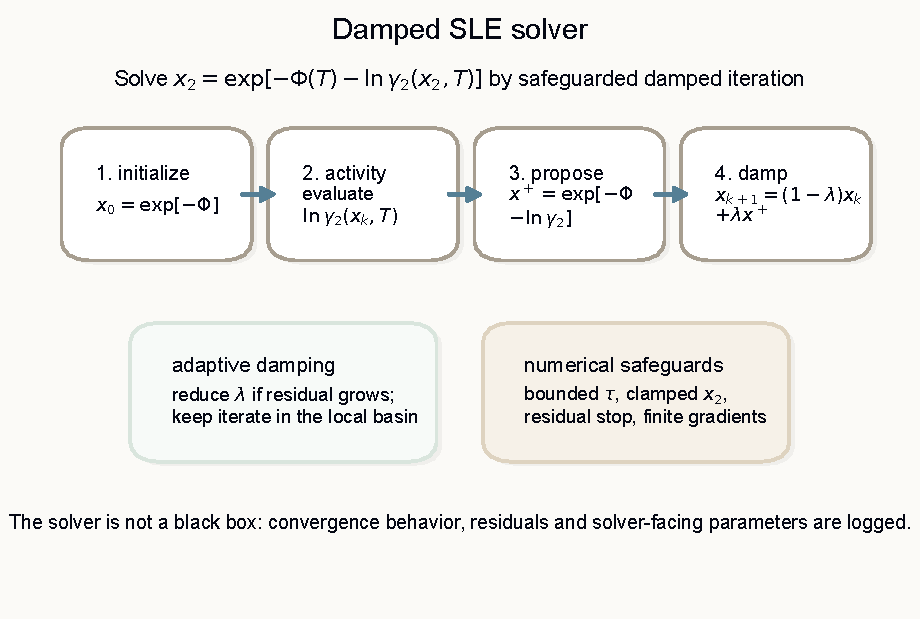
\includegraphics[width=0.96\textwidth]{figures/solver_convergence_schematic.pdf}
    \caption{Схема численного решения SLE как демпфированной итерации неподвижной точки. Все подписи на рисунке оставлены на английском языке, как и на остальных графиках отчёта.}
    \label{fig:solver-convergence-schematic}
\end{figure}

Существование решения следует из непрерывности $H(q)$ на усечённом интервале
$q\in[\ln\varepsilon,\ln(1-\varepsilon)]$. При ограниченных $\tau_{12},\tau_{21}$ и $\alpha$ коэффициент активности конечен. На левом конце $H(q)$ отрицателен за счёт $q\to-\infty$, а около $q=0$ для твёрдого вещества при $T<T_m$ обычно $\Phi(T)>0$, поэтому $H(q)$ положителен. Значит, корень существует по теореме о промежуточном значении. Единственность обеспечивается достаточным условием
\begin{equation*}
    H'(q)=1+x_2\frac{\partial \ln\gamma_2}{\partial x_2} \geq \mu>0.
\end{equation*}
Это условие проверяемо численно и физически естественно: в области малой растворимости $x_2$ подавляет производную активности, а NRTL-параметры в модели ограничены. Если в отдельных точках знаменатель неявной производной становится слишком мал, обратный проход дополнительно ограничивает
$|1+x_2\eta|$ снизу, где $\eta=\partial\ln\gamma_2/\partial x_2$. Это не меняет прямое предсказание, но предотвращает нефизический взрыв градиента.

Чтобы итерации не осциллировали при плохих ранних параметрах, используется демпфирование:
\begin{equation*}
    x^{(k+1)}
    =\lambda_k G(x^{(k)})+(1-\lambda_k)x^{(k)},
    \qquad 0<\lambda_k\leq 1.
\end{equation*}
Если $G'(x)$ лежит в интервале $[m,M]$ и $M<1$, то производная демпфированной карты равна
$(1-\lambda)+\lambda G'(x)$. При выборе
\begin{equation*}
    0<\lambda<\frac{2}{1-m}
\end{equation*}
она по модулю меньше единицы для отрицательных $m$, что устраняет типичную двухточечную осцилляцию. В реализации начальное $\lambda=0.7$, минимальное $0.1$; если логарифмический остаток растёт, шаг уменьшается вдвое, а если остаток падает, шаг медленно увеличивается. Поэтому демпфирование работает как локальный line-search для неподвижной точки.

Неявное дифференцирование записывается для функции
\begin{equation*}
    F(x_2,\theta)=x_2\gamma_2(x_2,T;\theta)-\exp[-\Phi(T)] .
\end{equation*}
По теореме о неявной функции
\begin{equation*}
    \frac{\partial x_2^*}{\partial\theta}
    =-
    \frac{\partial F/\partial\theta}{\partial F/\partial x_2}.
\end{equation*}
Так как
\begin{equation*}
    \frac{\partial F}{\partial x_2}
    =\gamma_2\left(1+x_2\frac{\partial\ln\gamma_2}{\partial x_2}\right),
\end{equation*}
то в логарифмической переменной существенный знаменатель имеет вид
$1+x_2\eta$. Именно этот множитель диагностировался как возможное узкое место градиента через физический слой.

Численная точность контролируется остатком
\begin{equation*}
    r_k=|\ln G(x^{(k)})-\ln x^{(k)}|.
\end{equation*}
В режиме сжатия с константой $L<1$ ошибка после $k$ итераций удовлетворяет стандартной оценке
\begin{equation*}
    |q_k-q^*|\leq \frac{L}{1-L}|q_k-q_{k-1}|.
\end{equation*}
Поскольку метрика отчёта сама является ошибкой в $q=\ln x_2$, эта величина напрямую измеряет вклад численного решателя в MAE. Ограничения $x_2\in[10^{-10},1-10^{-10}]$ защищают от переполнения и логарифма нуля; в выводах отчёта это означает, что численная ошибка решателя существенно меньше наблюдаемого модельного разрыва порядка $1$--$2$ в $\ln x_2$.

\section{Чувствительность к кристаллическим параметрам}
\label{app:sensitivity}

В приближении $\Delta C_p=0$ и при фиксированном $\gamma_2$:
\begin{equation*}
    \ln x_2=-\frac{\dHfus}{R}\left(\frac{1}{T}-\frac{1}{\Tm}\right)-\ln\gamma_2.
\end{equation*}
Тогда
\begin{align*}
    \frac{\partial \ln x_2}{\partial \Tm}
    &=-\frac{\dHfus}{R\Tm^2}, \\
    \frac{\partial \ln x_2}{\partial \dHfus}
    &=-\frac{1}{R}\left(\frac{1}{T}-\frac{1}{\Tm}\right).
\end{align*}

\begin{estimate}[Ошибка температуры плавления]
Пусть $\dHfus=30\,\mathrm{kJ/mol}$, $\Tm=450\,\mathrm{K}$, ошибка $\delta\Tm=30\,\mathrm{K}$. Тогда
\begin{equation*}
    \abs{\delta\ln x_2}
    \approx \frac{30000}{8.314\cdot 450^2}\cdot 30
    \approx 0.53.
\end{equation*}
Только ошибка $\Tm$ порядка $30\,\mathrm{K}$ способна дать вклад около $0.5$ в $\ln x_2$.
\end{estimate}

\begin{estimate}[Ошибка энтальпии плавления]
Пусть $T=298\,\mathrm{K}$, $\Tm=450\,\mathrm{K}$, ошибка $\delta\dHfus=5\,\mathrm{kJ/mol}$. Тогда
\begin{equation*}
    \abs{\delta\ln x_2}
    \approx \frac{5000}{8.314}\left(\frac{1}{298}-\frac{1}{450}\right)
    \approx 0.68.
\end{equation*}
Следовательно, даже умеренная ошибка $\dHfus$ может быть сопоставима с целевой ошибкой всей модели.
\end{estimate}

Эти оценки объясняют, почему физический путь может проигрывать прямой модели: ошибка промежуточных физических параметров усиливается при прохождении через уравнение равновесия.

\begin{figure}[H]
\centering
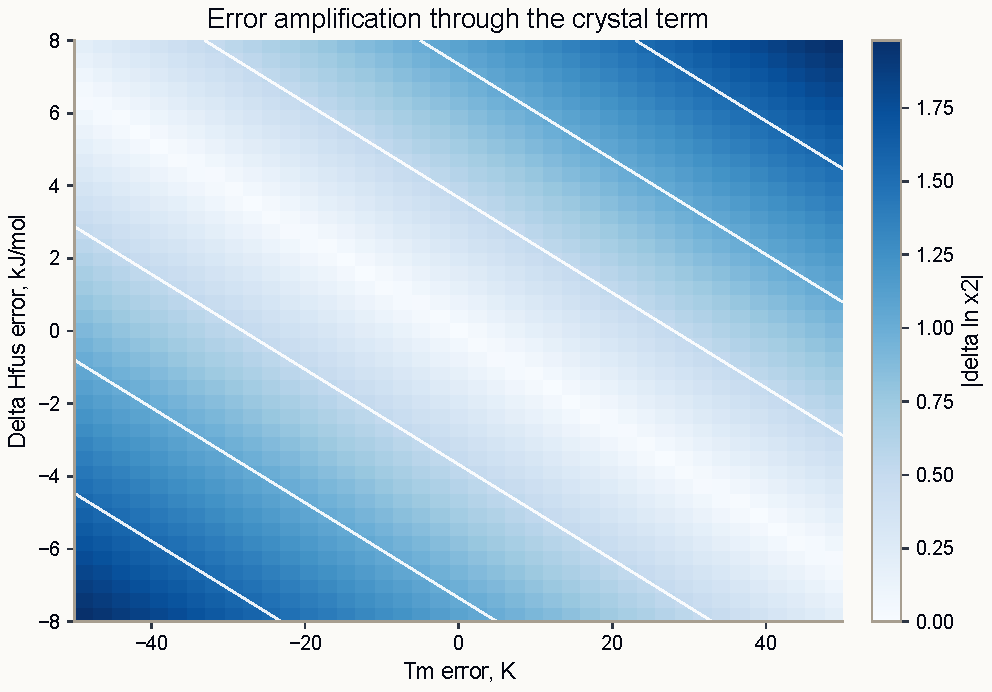
\includegraphics[width=0.84\textwidth]{sensitivity_heatmap.pdf}
\caption{Чувствительность $\ln x_2$ к ошибкам кристаллических параметров. Даже умеренные ошибки $\Tm$ и $\dHfus$ способны дать вклад того же порядка, что и весь целевой выигрыш между моделями.}
\label{fig:sensitivity-heatmap}
\end{figure}

\section{Вант-Гофф, температурные наклоны и кондиционирование}
\label{app:vant-hoff}

Если энтальпия растворения приблизительно постоянна, то
\begin{equation*}
    \frac{\partial \ln x_2}{\partial (1/T)}\approx -\frac{\Delta H_{\mathrm{sol}}}{R}.
\end{equation*}
Для одной пары линейная регрессия
\begin{equation*}
    \ln x_2 = a + b\frac{1}{T}
\end{equation*}
даёт оценку
\begin{equation*}
    \Delta H_{\mathrm{sol}}\approx -Rb.
\end{equation*}

\begin{estimate}[Физический смысл ошибки наклона]
Если ошибка наклона равна $1600\,\mathrm{K}$, то ошибка эффективной энтальпии растворения составляет
\begin{equation*}
    \abs{\delta\Delta H_{\mathrm{sol}}}
    \approx R\cdot 1600
    \approx 8.314\cdot 1600
    \approx 13.3\,\mathrm{kJ/mol}.
\end{equation*}
Это химически существенная величина, сравнимая с изменением нескольких сильных межмолекулярных контактов.
\end{estimate}

\begin{estimate}[Почему близкие температуры плохо определяют наклон]
Пусть есть три точки в узком диапазоне $298$--$310\,\mathrm{K}$. Тогда диапазон переменной $u=1/T$ равен
\begin{equation*}
    \Delta u = \frac{1}{298}-\frac{1}{310}\approx 1.30\times10^{-4}\,\mathrm{K}^{-1}.
\end{equation*}
Для трёх приблизительно равномерных точек
\begin{equation*}
    S_{uu}=\sum_i(u_i-\bar u)^2 \approx \frac{(\Delta u)^2}{2}
    \approx 8.5\times10^{-9}\,\mathrm{K}^{-2}.
\end{equation*}
Если шум $\ln x_2$ имеет стандартное отклонение всего $\sigma=0.1$, то стандартная ошибка наклона порядка
\begin{equation*}
    \mathrm{SE}(b)\approx \frac{\sigma}{\sqrt{S_{uu}}}
    \approx \frac{0.1}{9.2\times10^{-5} }
    \approx 1.1\times10^3\,\mathrm{K}.
\end{equation*}
Поэтому даже физически правильная модель может плохо восстанавливать температурный наклон, если температурный диапазон узок или измерения шумны.
\end{estimate}

\section{Идентифицируемость кристалла и активности}
\label{app:identifiability}

Линеаризуем модель по параметрам, отвечающим за температурный наклон. Упрощённо:
\begin{equation*}
    \ln x_2(T)
    \approx c_0
    -\frac{\dHfus}{R}\left(\frac{1}{T}-\frac{1}{\Tm}\right)
    -\beta_{\gamma}\left(\frac{1}{T}-\frac{1}{T_{\mathrm{ref}}}\right),
\end{equation*}
где $\beta_{\gamma}$ обозначает эффективный температурный вклад активности. Обе величины $\dHfus$ и $\beta_{\gamma}$ умножаются на функции, близкие к линейным по $1/T$. При узком температурном диапазоне столбцы соответствующей матрицы чувствительности почти коллинеарны.

Пусть вектор наблюдений $y$ аппроксимируется как
\begin{equation*}
    y\approx X\theta,\qquad
    \theta=(\dHfus,\beta_{\gamma},c_0)^\top.
\end{equation*}
Дисперсия оценки в линейной модели пропорциональна
\begin{equation*}
    \Var(\widehat\theta)\propto (X^\top X)^{-1}.
\end{equation*}
Если $X^\top X$ плохо обусловлена, малый шум в $y$ даёт большой разброс в $\widehat\theta$. Именно это и есть компенсаторная вырожденность: кристаллическая часть и активность могут взаимно поглощать ошибки друг друга, сохраняя похожее $\ln x_2$.

Отсюда следует практическое требование: одних SLE-строк недостаточно. Нужны дополнительные сигналы, которые отдельно ограничивают кристаллические свойства и активность. В проекте эту роль выполняют $\Tm$, $\dHfus$, IDAC, UNIFAC, параметры Хансена и температурные кривые.

\section{Формальная запись предобучения и функции ошибки}
\label{app:loss-pretraining}

Этап 0 можно записать как многозадачное обучение графового блока $h_\theta(G)$ на молекулярных графах без целевой растворимости:
\begin{equation*}
    \mathcal L_{\mathrm{stage0}}
    = \lambda_{\mathrm{atom}}\mathcal L_{\mathrm{atom}}
    + \lambda_{\mathrm{bond}}\mathcal L_{\mathrm{bond}}
    + \lambda_{\mathrm{desc}}\mathcal L_{\mathrm{desc}}
    + \lambda_{\mathrm{contr}}\mathcal L_{\mathrm{contr}}.
\end{equation*}
Для маскированных атомных признаков используется классификационная или смешанная классификационно-регрессионная ошибка по скрытым признакам:
\begin{equation*}
    \mathcal L_{\mathrm{atom}}
    = -\sum_{i\in M_{\mathrm{atom}}}\log p_\theta(a_i\mid G_{\setminus M}).
\end{equation*}
Для типа связи:
\begin{equation*}
    \mathcal L_{\mathrm{bond}}
    = -\sum_{(i,j)\in M_{\mathrm{bond}}}\log p_\theta(b_{ij}\mid G_{\setminus M}).
\end{equation*}
Для дескрипторов:
\begin{equation*}
    \mathcal L_{\mathrm{desc}}
    = \left\| W_{\mathrm{desc}} h_\theta(G)-d(G)\right\|_2^2,
\end{equation*}
где $d(G)$ --- нормированный вектор RDKit-дескрипторов. Контрастивная часть может быть записана в форме InfoNCE:
\begin{equation*}
    \mathcal L_{\mathrm{contr}}
    =-\log
    \frac{\exp(\operatorname{sim}(z_i,z_i^+)/\tau)}
    {\exp(\operatorname{sim}(z_i,z_i^+)/\tau)+
     \sum_j\exp(\operatorname{sim}(z_i,z_j^-)/\tau)}.
\end{equation*}
Здесь $z$ --- проекция молекулярного представления, $z_i^+$ --- другая аугментированная версия той же молекулы, $z_j^-$ --- отрицательные примеры.

Основная функция обучения TGNN-Solv после этапа 0 имеет вид
\begin{equation*}
    \mathcal L_{\mathrm{TGNN}}
    = \sum_k \lambda_k^{(p)} \mathcal L_k,
\end{equation*}
где $p$ обозначает фазу обучения. Фазовая зависимость весов не является косметической деталью: при $p=1$ доминируют кристаллические и вспомогательные свойства, при $p=2$ доминирует растворимость, при $p=3$ уменьшается шаг оптимизации и остаются физические ограничения.

Если для строки отсутствует вспомогательная метка, соответствующий член выключается маской:
\begin{equation*}
    \mathcal L_T
    = \frac{\sum_i m_i^T \rho(\widehat T_{m,i}-T_{m,i})}
           {\sum_i m_i^T+\varepsilon}.
\end{equation*}
Такой вид принципиален: отсутствующие физические свойства не должны превращаться в искусственные нули.

Для температурных рядов одной пары можно ввести локальное ограничение на наклон. Пусть $u=1/T$ и для пары $r$ известна оценка наклона $b_r$ из обучающих точек. Тогда вспомогательный член можно записать как
\begin{equation*}
    \mathcal L_{\mathrm{slope}}
    = \sum_r \rho\!\left(
        \frac{\widehat{\ln x_2}(u_{r,2})-\widehat{\ln x_2}(u_{r,1})}
             {u_{r,2}-u_{r,1}}
        - b_r
    \right),
\end{equation*}
если в мини-пакете или в специальном якорном наборе есть две температуры одной пары. Этот член напрямую проверяет то, что оказалось главным температурным провалом кратких запусков: восстановление физического наклона, а не только точечного значения.

\section{Математическое обоснование предложенных доработок}
\label{app:improvements}

\subsection{Отдельный IDAC-поток}

Из \eqref{eq:idac} следует, что IDAC ограничивает комбинацию параметров NRTL. Если добавлять IDAC как обычную строку растворимости, возникает неверная постановка: у такой строки нет SLE-измерения $\ln x_2$. Поэтому корректный путь --- отдельный вспомогательный член функции обучения:
\begin{equation*}
    \mathcal L_{\mathrm{IDAC}}
    = w_{\mathrm{exp}}\,\rho\!
    \left(\widehat{\ln\gamma_2^{\infty}}-\ln\gamma_{2,\mathrm{exp}}^{\infty}\right),
\end{equation*}
где $\rho$ --- робастная ошибка, например Хьюбера. Для псевдометок UNIFAC вес должен быть меньше:
\begin{equation*}
    w_{\mathrm{UNIFAC}}<w_{\mathrm{exp}}.
\end{equation*}
В текущих артефактах используется отношение $0.15$ против $1.0$.

\subsection{UNIFAC как приор}

Пусть детерминированная групповая модель даёт оценку $\tau^{(0)}$ или, слабее, оценку $\ln\gamma^\infty$. Тогда нейросетевая модель может учить не полный параметр из нуля, а поправку:
\begin{equation*}
    \tau_{ij}=\tau_{ij}^{(0)}+\Delta\tau_{ij}^{\mathrm{NN}}.
\end{equation*}
Если $\tau_{ij}^{(0)}$ имеет меньшую ошибку на новых функциональных группах, чем случайная инициализация или чисто нейросетевая экстраполяция, то задача обучения поправки проще:
\begin{equation*}
    \E\abs{\Delta\tau_{ij}^{\mathrm{NN}}}
    < \E\abs{\tau_{ij}^{\mathrm{NN}}}.
\end{equation*}
Это и есть смысл приора: он не обязан быть точным, но должен уменьшать радиус поиска для параметров активности.

\subsection{Разделение кристаллической и парной информации}

Пусть общий графовый блок имеет параметры $\theta$. Тогда градиент общей функции обучения имеет вид
\begin{equation*}
    \nabla_\theta \mathcal L
    =\lambda_c\nabla_\theta\mathcal L_{\mathrm{crystal}}
    +\lambda_a\nabla_\theta\mathcal L_{\mathrm{activity}}
    +\lambda_s\nabla_\theta\mathcal L_{\mathrm{SLE}}.
\end{equation*}
Если $\mathcal L_{\mathrm{crystal}}$ имеет гораздо больше прямых меток и меньший шум, то этот градиент может доминировать. Но признаки, полезные для $\Tm$ и упаковки кристалла, не обязаны совпадать с признаками, полезными для жидкофазной совместимости пары.

Математически это конфликт направлений градиента. Если
\begin{equation*}
    \cos\angle(\nabla\mathcal L_{\mathrm{crystal}},\nabla\mathcal L_{\mathrm{activity}})<0
\end{equation*}
или близок к нулю, общий блок получает компромиссный сигнал. Поэтому обоснованы режимы разделения представлений: отдельные адаптеры или частичное отключение кристаллического градиента во второй фазе.

\begin{figure}[H]
\centering
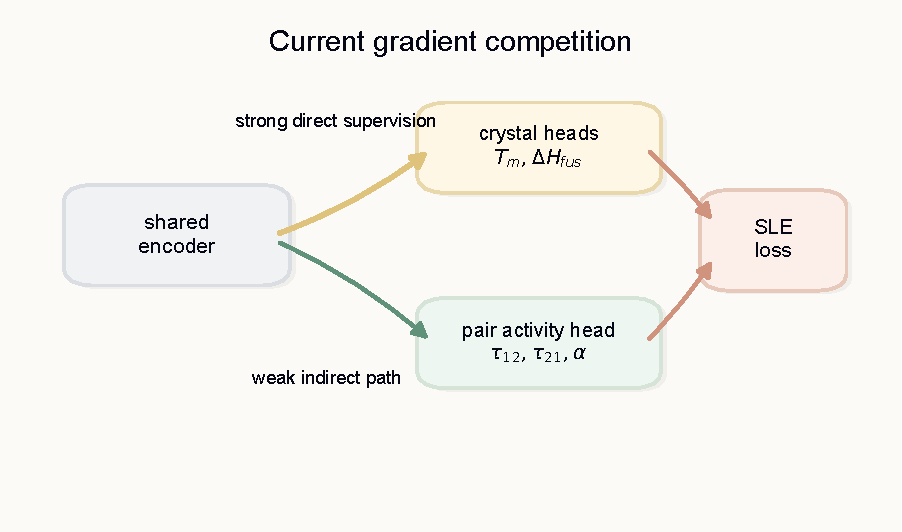
\includegraphics[width=0.92\textwidth]{gradient_flow.pdf}
\caption{Диагностика конфликта градиентов. Кристаллический сигнал проще, и для него чаще есть прямые метки, поэтому он может перетягивать общий графовый блок в сторону признаков чистого твёрдого вещества.}
\label{fig:gradient-flow-diagnosis}
\end{figure}

\begin{figure}[H]
\centering
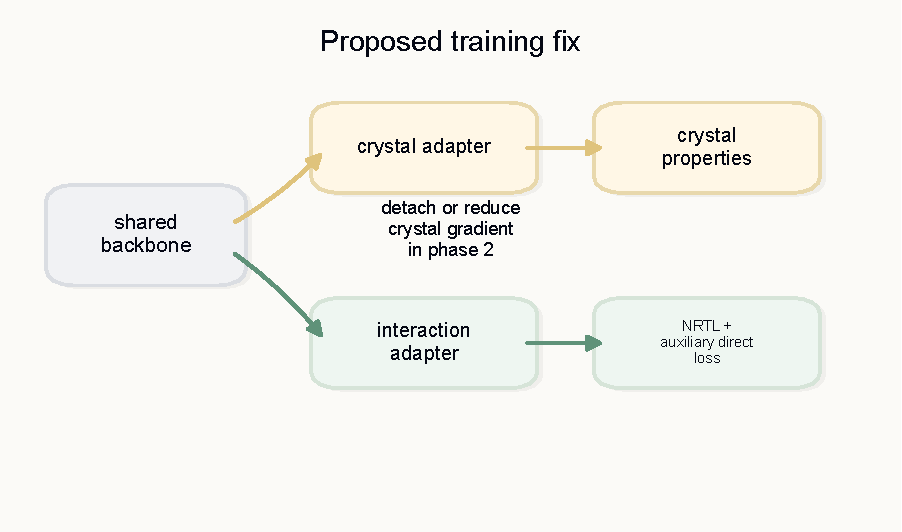
\includegraphics[width=0.92\textwidth]{gradient_flow_fix.pdf}
\caption{Предлагаемое исправление конфликта градиентов: разделение или частичное отключение кристаллического градиента во второй фазе должно усилить ветвь парного взаимодействия.}
\label{fig:gradient-flow-fix}
\end{figure}

\subsection{Парные параметры Хансена}

В теории параметров растворимости вклад смешения часто приближённо связан с квадратом расстояния между параметрами растворителя и растворённого вещества~\cite{hansen2007}:
\begin{equation*}
    \Delta E_{\mathrm{mix}} \propto
    (\delta_{d,2}-\delta_{d,1})^2+
    (\delta_{p,2}-\delta_{p,1})^2+
    (\delta_{h,2}-\delta_{h,1})^2.
\end{equation*}
Поэтому предсказывать только индивидуальные параметры недостаточно; важна именно разность или расстояние пары. Отсюда следует дополнительная функция обучения
\begin{equation*}
    \mathcal L_{\Delta HSP}
    =\left\|\widehat{\boldsymbol\delta_2-\boldsymbol\delta_1}
    -(\boldsymbol\delta_2-\boldsymbol\delta_1)\right\|_2^2.
\end{equation*}
Она напрямую обучает представление совместимости, а не только свойства отдельных молекул.

\subsection{Парное контрастивное предобучение}

Растворимость является парным свойством. Поэтому предобучение только на одиночных молекулах не учит совместимость. Для одного растворителя можно строить пары растворяемых веществ $A$ и $B$ и задавать метку
\begin{equation*}
    y_{AB}=\mathbb I\{\abs{\overline{\ln x_2(A)}-\overline{\ln x_2(B)}}<\varepsilon\}.
\end{equation*}
Тогда модель учит, какие вещества имеют похожую растворимость в одном и том же растворителе. Особенно важны трудные отрицательные примеры:
\begin{equation*}
    \mathrm{Tanimoto}(A,B)>0.6,
    \qquad
    \abs{\Delta\ln x_2}>2.0.
\end{equation*}
Такие пары показывают, что структурная похожесть не всегда означает близкую растворимость. В текущем артефакте найдено $204$ трудных отрицательных примера и $246$ простых положительных примеров при заданных порогах. Этого достаточно для начальной вспомогательной задачи, но не достаточно, чтобы объяснить всю структурную ошибку.

\section{Распространение ошибки через физический слой}
\label{app:error-propagation}

Пусть физическая модель задаёт отображение
\begin{equation*}
    \widehat y
    = f(\widehat \theta_c,\widehat \theta_a; T),
    \qquad
    y=\ln x_2,
\end{equation*}
где $\theta_c=(\Tm,\dHfus,\dCpfus,\ldots)$ --- кристаллические параметры, а $\theta_a=(\tau_{12},\tau_{21},\alpha,\ldots)$ --- параметры активности. В первом порядке ошибка предсказания равна
\begin{equation}
    \delta y
    \approx
    \nabla_{\theta_c}f^\top \delta\theta_c
    +
    \nabla_{\theta_a}f^\top \delta\theta_a.
    \label{eq:error-propagation}
\end{equation}
Для прямой модели аналогичного физического разложения нет: она сразу аппроксимирует $y$. Поэтому физическая модель может проигрывать прямой даже при правильной структуре уравнения, если ошибки промежуточных параметров велики.

В простом приближении $\Delta C_p=0$ и фиксированной активности
\begin{equation*}
    f(\theta_c,\theta_a;T)
    =
    -\frac{\dHfus}{R}\left(\frac{1}{T}-\frac{1}{\Tm}\right)
    -\ln\gamma_2.
\end{equation*}
Тогда вклад кристаллических ошибок:
\begin{equation*}
    \delta y_c
    \approx
    -\frac{\dHfus}{R\Tm^2}\delta \Tm
    -
    \frac{1}{R}\left(\frac{1}{T}-\frac{1}{\Tm}\right)\delta \dHfus.
\end{equation*}
Подставляя типичные значения $\dHfus=30\,\mathrm{kJ/mol}$, $\Tm=450\,\mathrm K$, $T=298\,\mathrm K$, получаем:
\begin{align*}
    \delta \Tm=30\,\mathrm K
    &\Rightarrow
    \abs{\delta y_T}\approx 0.53,\\
    \delta \dHfus=5\,\mathrm{kJ/mol}
    &\Rightarrow
    \abs{\delta y_H}\approx 0.68.
\end{align*}
Эти два вклада уже могут дать ошибку порядка $1$ в $\ln x_2$ до учёта активности.

Для активности в первом порядке:
\begin{equation*}
    \delta y_a=-\delta\ln\gamma_2.
\end{equation*}
Если NRTL-блок ошибается в $\ln\gamma_2$ всего на $0.5$--$1.0$, итоговая ошибка становится сравнимой с текущей разницей между сильными моделями. Поэтому физическая модель требует не просто правильного уравнения, а точного обучающего сигнала для промежуточных параметров.

\begin{figure}[H]
\centering
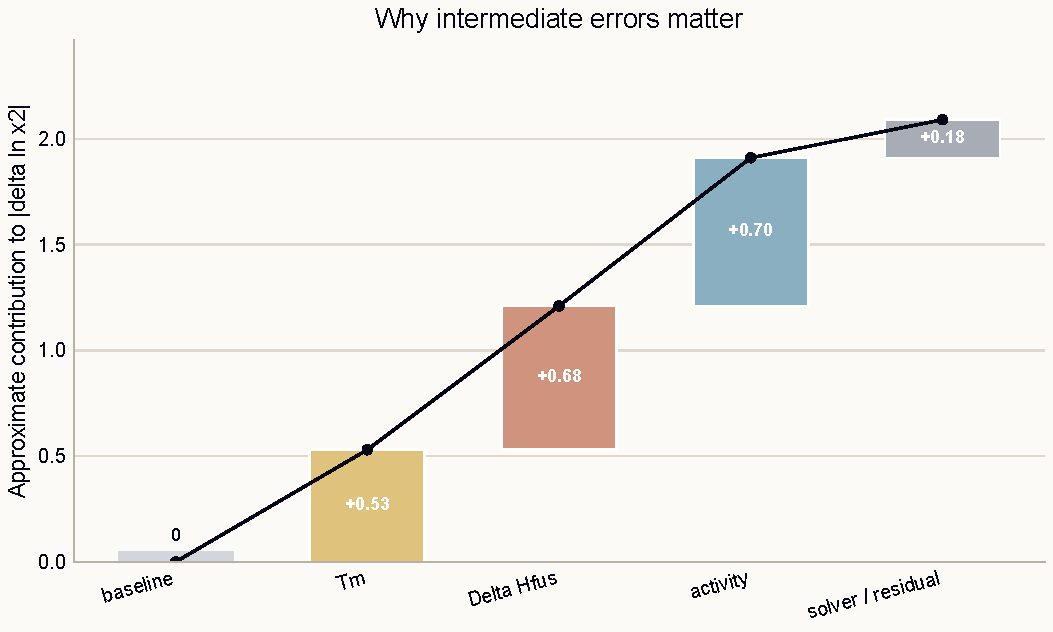
\includegraphics[width=0.84\textwidth]{error_decomposition_waterfall.pdf}
\caption{Схематическое распространение ошибок через физический слой. В TGNN-Solv ошибка промежуточных физических параметров может усиливаться до ошибки в $\ln x_2$, поэтому физическая корректность уравнения сама по себе не гарантирует низкий MAE.}
\label{fig:error-waterfall}
\end{figure}

\begin{claim}
Если промежуточные параметры физической модели имеют ошибку масштаба, указанного выше, то физический слой может дать больший MAE, чем прямая модель, даже если уравнение SLE термодинамически корректно.
\end{claim}

\begin{proof}
Достаточно применить линейное приближение \eqref{eq:error-propagation}. При типичных параметрах ошибка $30\,\mathrm K$ в $\Tm$ даёт вклад около $0.53$, ошибка $5\,\mathrm{kJ/mol}$ в $\dHfus$ --- около $0.68$. Эти величины аддитивны в первом порядке и сопоставимы с целевым MAE. Следовательно, физический путь чувствителен к качеству промежуточных предсказаний.
\end{proof}

\section{Одноатомный граф воды и почему явные водороды обоснованы}
\label{app:water}

В стандартной молекулярной графовой постановке водороды часто удаляются~\cite{landrum2024,gilmer2017}. Тогда вода, записанная как SMILES \code{O}, имеет один тяжёлый атом и ноль обычных связей между тяжёлыми атомами. Для слоя передачи сообщений вида
\begin{equation*}
    h_i^{(\ell+1)}
    =
    U_\ell\!\left(
        h_i^{(\ell)},
        \sum_{j\in\mathcal N(i)}
        M_\ell(h_i^{(\ell)},h_j^{(\ell)},e_{ij})
    \right)
\end{equation*}
у воды множество соседей пусто: $\mathcal N(i)=\varnothing$. Поэтому
\begin{equation*}
    h_O^{(\ell+1)}=U_\ell(h_O^{(\ell)},0).
\end{equation*}
Модель может использовать начальные признаки кислорода, но не может передавать информацию по O--H связям, потому что этих рёбер нет в графе.

Если добавить явные водороды для малых молекул, вода становится графом
\begin{equation*}
    \mathrm{H{-}O{-}H}.
\end{equation*}
Тогда появляются O--H рёбра, и полярность связи, донорно-акцепторные свойства и физические признаки ребра могут участвовать в передаче сообщений. Это особенно важно для TIMP-подобных каналов, где дисперсионная и полярная части зависят от признаков рёбер.

Эта модификация не является произвольной инженерной эвристикой. Она восстанавливает химические связи, которые были удалены ради стандартной графовой экономии, но для воды и других малых молекул содержат основную физическую информацию.

\section{Статистическая интерпретация текущего разрыва TGNN-Solv и DirectGNN}
\label{app:statistics}

Текущий разрыв на тесте по новым каркасам равен
\begin{equation*}
    \Delta_{\mathrm{MAE}}
    =
    \mae_{\mathrm{TGNN}}-\mae_{\mathrm{Direct}}
    =
    1.741-1.652
    =
    0.089.
\end{equation*}
Этот разрыв мал по сравнению с абсолютным уровнем ошибки, но он получен на согласованных предсказаниях и поэтому является содержательным. Для строки $i$ определим парную разность абсолютных ошибок:
\begin{equation*}
    d_i
    =
    \abs{\widehat y_i^{\mathrm{TGNN}}-y_i}
    -
    \abs{\widehat y_i^{\mathrm{Direct}}-y_i}.
\end{equation*}
Тогда
\begin{equation*}
    \Delta_{\mathrm{MAE}}=\frac{1}{n}\sum_{i=1}^n d_i.
\end{equation*}
Положительное значение означает проигрыш TGNN-Solv по средней абсолютной ошибке. Однако известно, что TGNN-Solv лучше DirectGNN примерно на $46.4\%$ строк. Следовательно, распределение $d_i$ не имеет одного знака: физическая модель выигрывает почти на половине строк, но проигрывает сильнее или чаще на оставшейся части.

Это обосновывает два вывода.

\begin{enumerate}
    \item Нельзя делать вывод только по одной общей MAE: нужна диагностика срезов, потому что модели дополняют друг друга.
    \item Нельзя делать сильный публикационный вывод по одному запуску: при разрыве $0.089$ требуются несколько случайных инициализаций и парные статистические проверки.
\end{enumerate}

Корректная проверка на нескольких случайных инициализациях должна рассматривать для каждой случайной инициализации величину
\begin{equation*}
    \Delta_s
    =
    \mae_{\mathrm{TGNN},s}
    -
    \mae_{\mathrm{Direct},s}.
\end{equation*}
После этого проверяется среднее $\bar\Delta$ и доверительный интервал. Минимальная практическая схема --- $3$ случайные инициализации, более надёжная --- $5$ случайных инициализаций. Без таких повторов нельзя отделить устойчивый эффект физического ограничения от вариации обучения.

\section{Почему структурная экстраполяция труднее температурной}
\label{app:structural-vs-temperature}

Температурная экстраполяция внутри одной пары и структурная экстраполяция на новый каркас являются разными задачами~\cite{hildebrand1970,apelblat1999,vermeire2022}.

Внутри одной пары функциональная форма зависимости от температуры приближённо известна:
\begin{equation*}
    \ln x_2(T) \approx a+b\frac{1}{T}.
\end{equation*}
После оценки $a$ и $b$ по нескольким точкам задача становится двумерной регрессией с сильным физическим ограничением. Поэтому Вант-Гофф даёт $\mae=0.368$.

Для нового каркаса неизвестны сами параметры пары:
\begin{equation*}
    (\tau_{12},\tau_{21},\alpha)
    =
    F(\mathrm{solute},\mathrm{solvent}).
\end{equation*}
Физика задаёт форму SLE-уравнения, но не сообщает значения $F$ для новой химической области. Поэтому структурная экстраполяция требует хорошего химического представления и переносимых приоров. Это объясняет, почему физика может быть очень сильной по температуре и одновременно не давать автоматического выигрыша на новых каркасах.

Формально можно записать ошибку на новом каркасе как сумму двух частей:
\begin{equation*}
    \abs{\widehat y-y}
    \le
    \underbrace{\abs{f(\widehat\theta,T)-f(\theta^\star,T)}}_{\text{ошибка параметров}}
    +
    \underbrace{\abs{f(\theta^\star,T)-y}}_{\text{ошибка физической модели}}.
\end{equation*}
Даже если второй член мал, первый может быть большим, если сеть плохо предсказывает параметры активности для новой химии. Именно поэтому расширение IDAC, UNIFAC-приоры, парное предобучение и раздельные представления кристалла/взаимодействия являются не украшениями, а прямыми средствами уменьшения первого члена.

\section{Связь параметров Хансена с парной совместимостью}
\label{app:hansen}

Параметры Хансена раскладывают энергию когезии на дисперсионный, полярный и водородно-связанный вклады~\cite{hansen2007}:
\begin{equation*}
    \boldsymbol\delta
    =
    (\delta_d,\delta_p,\delta_h).
\end{equation*}
Расстояние совместимости часто записывается в виде
\begin{equation*}
    R_a^2
    =
    4(\delta_{d,2}-\delta_{d,1})^2
    +(\delta_{p,2}-\delta_{p,1})^2
    +(\delta_{h,2}-\delta_{h,1})^2.
\end{equation*}
Чем меньше $R_a$, тем ближе вещества по параметрам растворимости и тем выше ожидаемая совместимость, при прочих равных условиях. Поэтому вспомогательная задача должна учить не только отдельные $\boldsymbol\delta_1$ и $\boldsymbol\delta_2$, но и их разность:
\begin{equation*}
    \mathcal L_{\mathrm{Hansen}\Delta}
    =
    \left\|
    \widehat{(\boldsymbol\delta_2-\boldsymbol\delta_1)}
    -
    (\boldsymbol\delta_2-\boldsymbol\delta_1)
    \right\|_2^2.
\end{equation*}
Это согласуется с физической целью: модель должна кодировать совместимость пары, а не только свойства отдельных молекул.



\section{TIMP: физическая декомпозиция передачи сообщений}
\label{app:timp-math}

Обычная графовая сеть передаёт одно сообщение по каждому ребру. Для растворимости это слишком грубо: вклад дисперсионных взаимодействий и вклад полярных взаимодействий имеют разную физическую природу и по-разному связаны с параметрами растворимости. Поэтому в варианте TIMP сообщение раскладывается на два канала \cite{gilmer2017,gasteiger2020,hansen2007}:
\begin{equation*}
    \mathbf m_{ij}
    =
    \mathbf m_{ij}^{\mathrm{disp}}
    +
    \mathbf m_{ij}^{\mathrm{polar}} .
\end{equation*}
Дисперсионный канал соответствует лондоновскому члену $E_{\mathrm{disp}}\sim-C_6/r^6$. Для атомов $i,j$ коэффициент $C_6$ растёт с поляризуемостью, поэтому естественный масштаб сообщения задаётся как
\begin{equation*}
    s_{ij}^{\mathrm{disp}}
    =\sqrt{\alpha_i^{\mathrm{pol}}\alpha_j^{\mathrm{pol}}},
    \qquad
    \mathbf m_{ij}^{\mathrm{disp}}
    =s_{ij}^{\mathrm{disp}}\,\phi_{\mathrm d}
    (\mathbf h_i,\mathbf h_j,\mathbf e_{ij}).
\end{equation*}
Полярный канал, наоборот, должен реагировать на перераспределение заряда, различие электроотрицательностей и способность к водородным связям. В реализации это задаётся через физические признаки ребра: разность электроотрицательностей, разность ван-дер-ваальсовых радиусов, полярность связи, донорно-акцепторную маску и сложенные в тяжёлый атом заряды Гастайгера:
\begin{equation*}
    \mathbf m_{ij}^{\mathrm{polar}}
    =s_{ij}^{\mathrm{polar}}\,\phi_{\mathrm p}
    (\mathbf h_i,\mathbf h_j,\mathbf e_{ij}^{\mathrm{phys}}),
\end{equation*}
где $s_{ij}^{\mathrm{polar}}$ является гладкой положительной функцией зарядовой и донорно-акцепторной совместимости. Вектор атома обновляется суммой сообщений:
\begin{equation*}
    \mathbf h_i^{(\ell+1)}
    =U\!\left(
    \mathbf h_i^{(\ell)},
    \sum_{j\in\mathcal N(i)}
    [\mathbf m_{ij}^{\mathrm{disp}}\Vert \mathbf m_{ij}^{\mathrm{polar}}]
    \right).
\end{equation*}

Смысл этой конструкции виден через параметры Хансена. Компонента $\delta_d$ отвечает главным образом за дисперсионные взаимодействия, а $\delta_p$ и $\delta_h$ --- за полярность и водородные связи. Поэтому для TIMP введена канальная вспомогательная задача:
\begin{equation*}
    \mathcal L_{\mathrm{TIMP}}
    =
    \mathcal D(\mathbf g^{\mathrm{disp}},\delta_d)
    +
    \mathcal D(\mathbf g^{\mathrm{polar}},(\delta_p,\delta_h))
    +
    \lambda_{\perp}
    \left|
    \cos(\bar{\mathbf g}^{\mathrm{disp}},\bar{\mathbf g}^{\mathrm{polar}})
    \right| .
\end{equation*}
Здесь $\mathcal D$ --- попарное выравнивание расстояний в пространстве скрытых представлений и в пространстве физических параметров. Оно не заставляет сеть точно предсказывать параметры Хансена в каждой точке; оно требует более слабого и более полезного свойства: если две молекулы близки по дисперсионному параметру, их дисперсионные векторные представления должны быть близки, и аналогично для полярного канала.

\begin{figure}[t]
    \centering
    \includegraphics[width=0.86\textwidth]{figures/timp_hansen_diagnostics.pdf}
    \caption{Диагностика TIMP и контрастивного выравнивания по параметрам Хансена. Результат важен не как финальная метрика растворимости, а как проверка того, что каналы действительно кодируют разные физические свойства.}
    \label{fig:timp-hansen-appendix}
\end{figure}

Физическая связь с NRTL состоит в том, что
\begin{equation*}
    \tau_{ij}(T)=\frac{\Delta g_{ij}(T)}{RT}
\end{equation*}
является безразмерной локальной энергией контакта. Эта энергия не является одной скалярной причиной: в ней смешаны дисперсия, полярность, водородные связи, стерическое окружение и размер молекулы. TIMP не делает NRTL более сложным, но даёт NRTL-блоку более разложенное представление пары. Это особенно важно для структурной экстраполяции: новый каркас может быть неизвестен целиком, но его дисперсионные и полярные фрагменты часто уже встречались в обучении.

Ограничения TIMP также важны. Модель остаётся двумерной графовой моделью: она не видит явные конформации, упаковку растворителя и трёхмерную сетку водородных связей. Поэтому TIMP следует рассматривать не как замену 3D-моделированию, а как физически более аккуратный способ передать в графовую сеть те признаки, которые доступны из SMILES и RDKit.

\section{Почему используется NRTL и как сохраняется термодинамическая консистентность}
\label{app:nrtl-choice-gd}

Для бинарной неидеальной жидкости нужен слой, который одновременно достаточно гибок, дифференцируем и термодинамически согласован. Wilson-модель компактна, но плохо подходит для систем с сильной локальной неслучайностью и ограничена в описании расслаивания. UNIQUAC физически богаче, но требует надёжных объёмных и поверхностных параметров и усложняет идентифицируемость. UNIFAC хорош как группово-вкладный ориентир, но его покрытие по новым молекулам и группам не является полным. NRTL занимает промежуточное место: она явно моделирует локальную неслучайность, имеет небольшое число параметров и задаёт коэффициенты активности из единой функции избыточной свободной энергии \cite{renon1968,prausnitz1998}.

Последний пункт принципиален. Для бинарной смеси при фиксированных $T,P$ уравнение Гиббса--Дюгема требует
\begin{equation*}
    x_1\,d\ln\gamma_1+x_2\,d\ln\gamma_2=0 .
\end{equation*}
Если коэффициенты активности получены как производные одной молярной избыточной свободной энергии $g^E$,
\begin{equation*}
    \ln\gamma_i
    =
    \left(\frac{\partial (n g^E/RT)}{\partial n_i}\right)_{T,P,n_{j\ne i}},
\end{equation*}
то согласованность следует из однородности $n g^E$ по числам молей. NRTL удовлетворяет этому требованию: $\ln\gamma_1$ и $\ln\gamma_2$ вычисляются не независимыми нейросетями, а из общего набора $\tau_{12},\tau_{21},\alpha$.

В TGNN-Solv нейросеть предсказывает параметры NRTL, но не нарушает эту структуру. Поэтому сам слой активности остаётся термодинамически согласованным. Это отличие от прямой модели: DirectGNN может быть точной по MAE, но у неё нет встроенного аналога уравнения Гиббса--Дюгема. Поправочный блок TGNN-Solv также устроен через изменение физических параметров и повторное решение SLE, а не через произвольный сдвиг $\ln x_2$; благодаря этому корректировка остаётся ближе к термодинамической форме модели.

\section{Приоры, принудительная подстановка и коррекция ошибки в пространстве параметров}
\label{app:priors-teacher-correction}

В проекте используется общий принцип: если существует слабая физическая оценка $p(x)$, модель не должна заново учить абсолютное значение, а должна учить ограниченную поправку:
\begin{equation*}
    \hat y=p(x)+b\tanh r_\theta(x),
    \qquad |\hat y-p(x)|\leq b .
\end{equation*}
Так устроены кристаллические группово-вкладные приоры. Для $T_m$ поправка аддитивна, для $\Delta H_{fus}$ --- мультипликативна:
\begin{equation*}
    \widehat T_m=T_m^{\mathrm{GC}}+b_T\tanh r_T,
    \qquad
    \widehat{\Delta H}_{fus}=\Delta H_{fus}^{\mathrm{GC}}\,s(r_H),
\end{equation*}
где $s(r_H)$ ограничена заданным интервалом множителей. Последний слой остаточных ветвей инициализируется нулями, поэтому на старте модель точно равна приору. Раннее замораживание остаточных ветвей делает обучение в первой фазе похожим на калибровку, а не на немедленное разрушение физической оценки.

Для NRTL есть два более слабых источника априорной информации. Первый --- групповая Hansen-подобная априорная оценка: по счётчикам фрагментов строятся грубые $\delta_d,\delta_p,\delta_h$ и молярные объёмы, затем из расстояния $R_a$ формируется небольшой сдвиг $\tau_{12},\tau_{21}$. Второй --- UNIFAC-подобная априорная оценка по $\ln\gamma^\infty$: при малых симметричных $\tau$ приближение NRTL даёт
\begin{equation*}
    \ln\gamma_2^\infty
    =\tau_{21}+\tau_{12}\exp(-\alpha\tau_{12})
    \approx 2\tau,
\end{equation*}
поэтому внешнюю оценку $\ln\gamma^\infty$ можно перевести в слабое начальное смещение $\tau\approx\frac12\ln\gamma^\infty$. В реализации этот сдвиг ограничен, чтобы плохая внешняя априорная оценка не могла доминировать над данными.

Стохастическая подстановка истинных значений --- это разновидность принудительной подстановки для физического слоя. Если в строке есть экспериментальное $T_m$ или $\Delta H_{fus}$, то в обучении с вероятностью $p_e$ в решатель передаётся истинное значение, а не предсказание выходного блока:
\begin{equation*}
    \theta_{\mathrm{solver}}
    =M\theta_{\mathrm{exp}}+(1-M)\theta_\theta,
    \qquad M\sim\mathrm{Bernoulli}(p_e).
\end{equation*}
Это решает конкретную оптимизационную проблему: ветвь NRTL начинает видеть более правдоподобный кристаллический вклад и получает менее шумный градиент. При этом непосредственные предсказания кристаллического выходного блока остаются в выходе модели и продолжают штрафоваться собственными компонентами функции ошибки. Во второй фазе вероятность такой подстановки держится на базовом уровне, а в последние $\min(50,n_{\mathrm{epochs}})$ эпох линейно убывает до нуля:
\begin{equation*}
    p_e=p_0\left(1-
    \frac{e-e_0+1}{n_{\mathrm{anneal}}}
    \right)_+ .
\end{equation*}
В третьей фазе подстановка отключена. Поэтому финальная модель не зависит от истинных значений при применении.

Поправочный блок не добавляет произвольную прямую регрессию. Он строит новое состояние параметров
\begin{equation*}
    \theta' = \theta + \Delta\theta,
    \qquad
    |\Delta T_m|\leq 60\,\mathrm K,
    \quad
    |\Delta \Delta H/\Delta H|\leq0.25,
    \quad
    |\Delta\tau_{ij}|\leq2,
\end{equation*}
после чего SLE решается повторно. Если $q(\theta)=\ln x_2$ --- решение физического слоя, то в первом порядке
\begin{equation*}
    q(\theta')-q(\theta)
    \approx
    J_\theta\Delta\theta,
    \qquad
    J_\theta=\frac{\partial q}{\partial\theta}.
\end{equation*}
Следовательно, поправочный блок является ограниченным шагом по параметрам, который может компенсировать малые ошибки $T_m$, $\Delta H_{fus}$ и $\tau$, но не может полностью превратиться в DirectGNN. Финальная формула имеет вид
\begin{equation*}
    q_{\mathrm{final}}
    =q_{\mathrm{phys}}+(1-c)\,\mathrm{clip}
    \{q(\theta')-q_{\mathrm{phys}},[-B,B]\},
    \qquad c\in[0,1].
\end{equation*}
Начальное смещение сети доверия даёт $c\approx0.9$, а последний слой сети поправок инициализируется нулём. Поэтому стартовая модель почти полностью доверяет физике; поправка включается только если данные устойчиво показывают, что параметрическое решение нужно поправить.

\begin{figure}[t]
    \centering
    \includegraphics[width=0.86\textwidth]{figures/correction_loop_schematic.pdf}
    \caption{Остаточная коррекция в TGNN-Solv: корректируются физические параметры, затем SLE решается повторно. Это сделано специально, чтобы поправка не разрушала термодинамическую форму модели.}
    \label{fig:correction-loop-appendix}
\end{figure}

\section{Температурные компоненты функции ошибки и случай взрыва vH-local}
\label{app:vh-catastrophe}

Для пары с несколькими температурами естественно требовать, чтобы предсказания были близки к прямой Вант-Гоффа в координатах $q=\ln x_2$ и $u=1/T$. Локальный наклон между двумя соседними точками равен
\begin{equation*}
    s_i=\frac{q_{i+1}-q_i}{u_{i+1}-u_i} .
\end{equation*}
локальный штраф Вант-Гоффа ограничивает изменение этого наклона:
\begin{equation*}
    \mathcal L_{\mathrm{vH-local}}
    =\frac{1}{m-2}\sum_i (s_{i+1}-s_i)^2 .
\end{equation*}
Катастрофа возникает, когда две температуры почти совпадают. Тогда $|u_{i+1}-u_i|$ мало, а градиент по $q_i$ масштабируется как
\begin{equation*}
    \left|\frac{\partial \mathcal L}{\partial q_i}\right|
    =O\!\left(\frac{1}{|u_{i+1}-u_i|^2}\right).
\end{equation*}
Даже небольшой шум измерения или случайная ошибка ранней модели превращается в огромный градиент. Это не теоретическая тонкость: именно такой сценарий объясняет нестабильные ранние попытки усилить температурную физику.

Стабилизация была сделана в три уровня. Во-первых, включена группировка мини-пакетов по парам: один мини-пакет старается содержать несколько температур для одной и той же пары, иначе температурный компонент функции потерь либо равен нулю, либо строится на случайных сравнениях. Во-вторых, знаменатель $|\Delta(1/T)|$ ограничен снизу:
\begin{equation*}
    \Delta u_{\mathrm{safe}}
    =\operatorname{sign}(\Delta u)\max(|\Delta u|,u_{\min}),
    \qquad u_{\min}=10^{-4}\,\mathrm K^{-1},
\end{equation*}
а вклад одной пары ограничен сверху. В-третьих, компоненты наклона и свободного члена нормируются характерными масштабами, а веса температурных регуляризаторов оставлены малыми.

\begin{figure}[t]
    \centering
    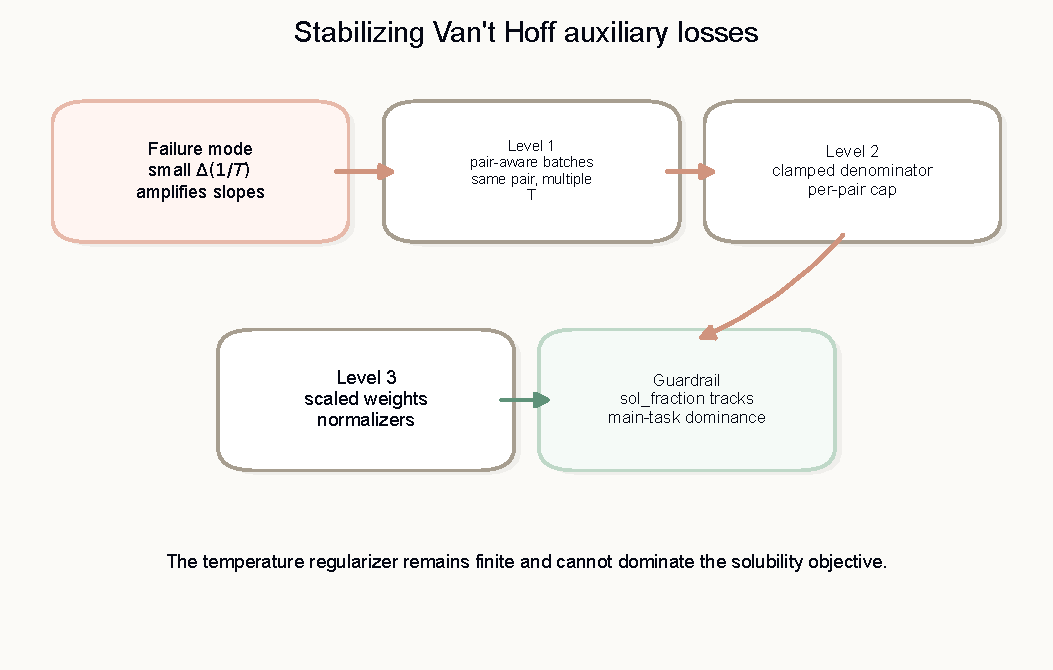
\includegraphics[width=0.96\textwidth]{figures/vh_stability_safeguards.pdf}
    \caption{Стабилизация температурных вспомогательных функций потерь. Главная цель --- не дать температурному регуляризатору вытеснить основной сигнал растворимости.}
    \label{fig:vh-stability-safeguards}
\end{figure}

Главный диагностический ограничитель --- доля ошибки по растворимости в полной функции потерь:
\begin{equation*}
    \mathrm{sol\_fraction}
    =
    \frac{\lambda_{\mathrm{sol}}\mathcal L_{\mathrm{sol}}}
    {\mathcal L_{\mathrm{total}}}.
\end{equation*}
Если эта величина падает ниже $0.1$, обучение фактически перестаёт оптимизировать целевую задачу и начинает подгонять регуляризаторы. Поэтому программа обучения печатает среднее и минимальное значение \code{sol\_fraction} по эпохе и отдельно предупреждает о доминировании регуляризаторов. В тестах для контрастивное выравнивание по параметрам Хансена пути дополнительно проверяется, что при малых весах контрастивная часть не вытесняет основную ошибку по растворимости.

\section{Группировка температурных наблюдений по парам}
\label{app:pair-aware-batching}

Температурные ограничения являются условными: они имеют смысл только внутри одной пары «вещество--растворитель». Если в мини-пакете лежат разные пары, сравнение $q(T_2)-q(T_1)$ смешивает температурный эффект с химическим различием. Поэтому загрузчик данных может группировать строки так, чтобы для части пар в мини-пакете присутствовало несколько температур. Формально цель переходит от независимой построчной регрессии
\begin{equation*}
    \sum_i \ell(f(s_i,v_i,T_i),q_i)
\end{equation*}
к смешанной задаче
\begin{equation*}
    \sum_i \ell_i
    +
    \sum_{(s,v)}
    \Omega\left(\{f(s,v,T_j):T_j\in\mathcal T_{s,v}\}\right),
\end{equation*}
где $\Omega$ задаёт монотонность, локальную линейность или совпадение с наклоном аппроксимации Вант-Гоффа. Это важное изменение протокола: оно делает физический компонент функции потерь наблюдаемым на уровне мини-пакета.

\section{Оптимизация, переобучение и балансировка регуляризации}
\label{app:optimization}

Основная оптимизация использует AdamW \cite{kingma2015,loshchilov2019}. Для градиента $g_t$ моменты обновляются как
\begin{equation*}
    m_t=\beta_1m_{t-1}+(1-\beta_1)g_t,
    \qquad
    v_t=\beta_2v_{t-1}+(1-\beta_2)g_t^2,
\end{equation*}
после чего применяется раздельное затухание весов:
\begin{equation*}
    \theta_{t+1}
    =\theta_t
    -\eta_t\frac{\hat m_t}{\sqrt{\hat v_t}+\varepsilon}
    -\eta_t\lambda_{\mathrm{wd}}\theta_t .
\end{equation*}
Для физической модели это особенно важно: параметры ветви решателя имеют разные масштабы, а обычный стохастический градиентный спуск плохо переносит смесь $T_m$, $\Delta H_{fus}$, $\tau$ и скрытых векторов. Перед шагом оптимизатора применяется ограничение нормы градиента
\begin{equation*}
    g\leftarrow g\min\left(1,\frac{c}{\|g\|_2}\right),
\end{equation*}
что защищает обучение от редких больших градиентов через решатель и температурные регуляризаторы.

Переобучение в этом проекте проявляется не только как разрыв между обучением и тестом. Для модели с физическими ограничениями есть второй тип переобучения: регуляризаторы могут стать слишком хорошими относительно основной задачи, а MAE по растворимости не улучшится. Поэтому логируются не только полная функция потерь и MAE, но и исходный и взвешенный вклад каждого компонента, \code{sol\_fraction}, максимальное отношение полной ошибки к ошибке по растворимости и число мини-пакетов, где регуляризаторы доминировали. Это инженерная, но необходимая часть математического контроля: многокомпонентная функция ошибки без таких диагностик неинтерпретируема.

\begin{figure}[t]
\centering
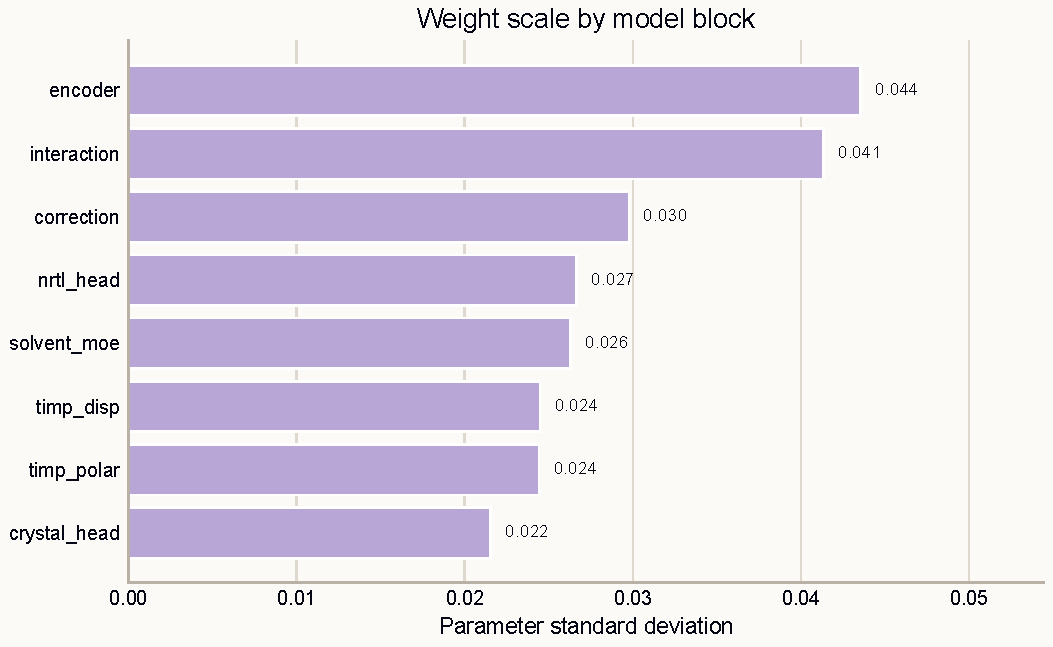
\includegraphics[width=0.86\textwidth]{weight_group_stats.pdf}
\caption{Диагностика масштабов весов по блокам модели. Она используется как грубый контроль того, не «умирает» ли отдельная ветвь и не доминирует ли один блок над остальной архитектурой после добавления новых регуляризаторов.}
\label{fig:weight-group-stats}
\end{figure}

Раннее прекращение обучения во второй и третьей фазах хранит лучшее состояние по валидационной средней абсолютной ошибке и восстанавливает его после остановки. Это важно для TGNN-Solv: поздние эпохи могут улучшать вспомогательные физические величины, но ухудшать целевую растворимость. Критерий остановки поэтому привязан к валидационному показателю, а не к сумме всех регуляризаторов.

\section{Гиперпараметрический поиск: Optuna, TPE и pruning}
\label{app:optuna}

Гиперпараметры подбирались не полным перебором. Пространство содержит категориальные и непрерывные параметры: размер скрытого слоя, число графовых и слоёв внимания, размер парного вектора, вероятность случайного выключения нейронов, шаг обучения, ограничение нормы градиента, режим $\tau(T)$, число экспертов в смеси экспертов, параметры GPS и дескрипторного расширения. Полный перебор по сетке был бы экспоненциально дорогим.

В Optuna стандартный байесовский механизм --- древовидная оценка Парзена (Tree-structured Parzen Estimator) \cite{akiba2019,bergstra2011}. Пусть уже выполнены испытания $(x_i,y_i)$, где $x_i$ --- гиперпараметры, а $y_i$ --- валидационный MAE. По квантилю $y^*$ испытания делятся на хорошие и плохие:
\begin{equation*}
    l(x)=p(x\mid y<y^*),
    \qquad
    g(x)=p(x\mid y\geq y^*).
\end{equation*}
Следующая точка выбирается так, чтобы увеличить отношение
\begin{equation*}
    \frac{l(x)}{g(x)}.
\end{equation*}
Это эквивалентно поиску точки с большой ожидаемой прибылью: гиперпараметры должны быть похожи на хорошие прогоны и непохожи на плохие. Для дорогих запусков может использоваться раннее отсечение неудачных запусков \cite{li2018}: испытание сообщает промежуточные значения, и если его траектория явно хуже уже наблюдавшихся, он останавливается до окончания планового прогона. В текущем коде основной модуль подбора минимизирует валидационный MAE; раннее отсечение не является центральным результатом, но математически совместим с тем же протоколом.

\begin{figure}[t]
    \centering
    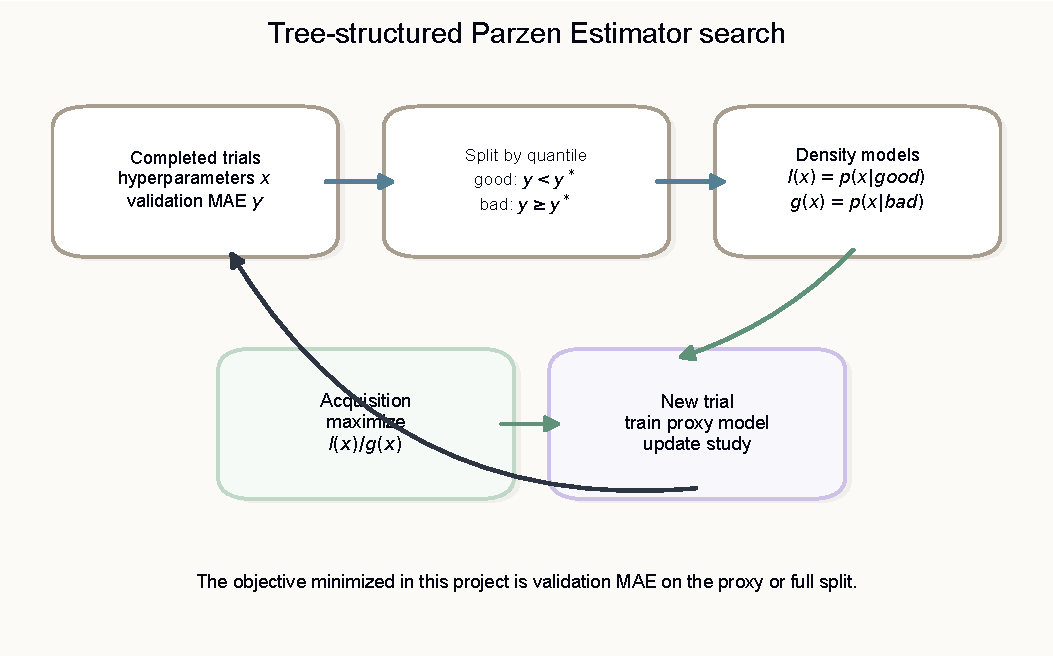
\includegraphics[width=0.96\textwidth]{figures/optuna_tpe_schematic.pdf}
    \caption{Схема TPE-поиска гиперпараметров. В отчёте результаты Optuna используются как источник настроенных конфигураций, а не как самостоятельное доказательство превосходства модели.}
    \label{fig:optuna-tpe-schematic}
\end{figure}

Результат поиска зафиксирован в наборах конфигураций \code{paper\_config\_tuned*}. Главное практическое следствие: настроенный DirectGNN оказался сильной контрольной моделью, а настроенный TGNN-Solv всё ещё платит небольшую цену за физический слой на разбиении по молекулярным каркасам. Поэтому последующие гипотезы нельзя проверять против слабой случайной конфигурации; сравнение должно идти против настроенного контроля.

\section{Дескрипторное расширение графового представления}
\label{app:descriptor-augmentation}

В проекте проверялся не только «чистый» графовый путь, но и гибридный вариант с RDKit-дескрипторами. Причина практическая: графовый блок может в принципе выучить молекулярную массу, число доноров водородной связи, полярную поверхность и липофильность, но заставлять его каждый раз восстанавливать эти величины из нуля не всегда эффективно. Дескрипторы добавляют известные химические координаты как явные признаки, а графовая часть остаётся ответственной за структуру и контекст взаимодействия.

Пусть $d_s$ и $d_v$ --- нормированные векторы дескрипторов растворяемого вещества и растворителя. Нормировка считается только по обучающей выборке:
\begin{equation*}
    \tilde d=\frac{d-\mu_{\mathrm{train}}}{\sigma_{\mathrm{train}}+\varepsilon}.
\end{equation*}
В парное представление подаются не только сами дескрипторы, но и простые взаимодействия:
\begin{equation*}
    d_{\mathrm{pair}}
    =
    [\tilde d_s,\tilde d_v,\tilde d_s-\tilde d_v,
      |\tilde d_s-\tilde d_v|,\tilde d_s\odot \tilde d_v].
\end{equation*}
После малой проекционной сети этот вектор добавляется к скрытому парному вектору и снова приводится к размерности \code{pair\_dim}. Такой путь не подменяет физическую модель: SLE-решатель, NRTL-блок и кристаллический выходной блок остаются теми же. Он только даёт выходным блокам более доступные химические координаты.

Важно, что дескрипторы не являются бесплатным решением структурной экстраполяции. Они помогают там, где нужное свойство действительно выражается через известные глобальные координаты. Но локальные эффекты, например различие положений заместителей, водородно-связанные мотивы и ассоциация растворителя, всё равно требуют графового или физического представления. Поэтому дескрипторные конфигурации рассматриваются как сильные гибридные абляции, а не как замена TGNN-Solv.

\section{Контракт воспроизводимых артефактов}
\label{app:artifact-contract}

Отдельная инженерная часть проекта --- единый контракт артефактов. Он нужен для того, чтобы результат эксперимента можно было проверить без устных пояснений. Минимальная запись одного запуска имеет вид
\begin{equation*}
    \mathcal A
    =
    (D_{\mathrm{train}},D_{\mathrm{val}},D_{\mathrm{test}},
     C,s,\theta,M,P,R),
\end{equation*}
где $D$ --- конкретные CSV-разбиения, $C$ --- конфигурация, $s$ --- начальное зерно генератора случайных чисел, $\theta$ --- сохранённое состояние модели, $M$ --- метрики, $P$ --- предсказания, $R$ --- манифест запуска с версией кода и окружением. Для наборов сравнительной оценки дополнительно сохраняется карточка эксперимента: какие модели сравнивались, какая целевая величина использовалась, были ли фильтры по единицам, какие строки исключены как нечисловые.

Такой контракт особенно важен для этого проекта, потому что часть отрицательных результатов связана не с архитектурой, а с протоколом: преобразование единиц, добавление IDAC-строк напрямую в SLE-таблицу, изменение валидационной и тестовой частей, сокращённый бюджет вместо полного обучения. Если артефакт не содержит разбиений, конфигурации и предсказаний, то нельзя понять, является ли изменение качества научным эффектом или сменой протокола.

\section{Линейная проба как проверка качества представлений}
\label{app:linear-probe}

Линейная проба отвечает на вопрос: насколько химически осмысленная информация уже линейно доступна в замороженном векторном представлении. Пусть $Z\in\mathbb R^{n\times d}$ --- матрица векторных представлений, а $Y\in\mathbb R^{n\times k}$ --- RDKit-дескрипторы или физические свойства. Обучается гребневая регрессия
\begin{equation*}
    W^*=(Z^\top Z+\lambda I)^{-1}Z^\top Y.
\end{equation*}
Если $R^2$ высок на обучающей части, но резко падает на тесте по новым каркасам, представление кодирует свойства только внутри виденных каркасов. Если $R^2$ сохраняется, проблема скорее находится в выходных блоках или физическом ограничительном слое.

В экспериментах TIMP и контрастивного выравнивания по параметрам Хансена этот тест использовался как диагностический, а не как финальная метрика. Он показывает, что канальное выравнивание улучшает доступность физико-химических координат в векторном представлении и уменьшает коллапс дисперсионного и полярного каналов. Это согласуется с гипотезой, что структурная экстраполяция требует не только большего набора данных, но и более переносимого пространства признаков.

\begin{figure}[t]
\centering
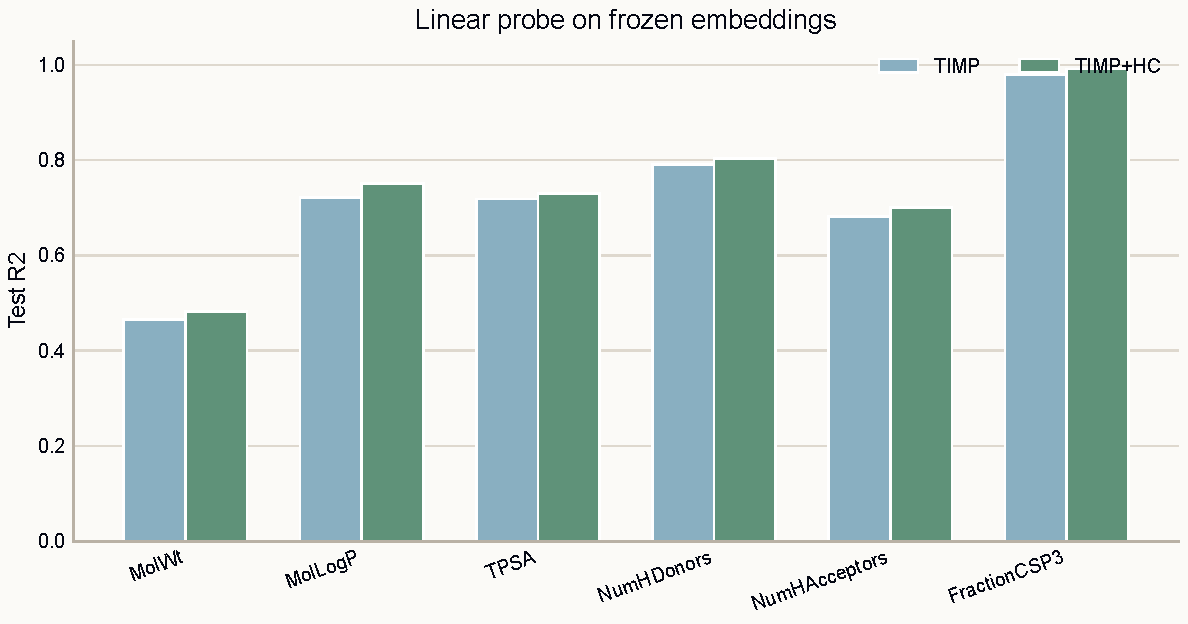
\includegraphics[width=0.88\textwidth]{descriptor_probe_bars.pdf}
\caption{Пример линейной диагностической пробы для TIMP-вариантов. Высокий $R^2$ по простым RDKit-дескрипторам означает, что соответствующая химическая координата линейно доступна в замороженном представлении; низкий $R^2$ указывает, что свойство либо не закодировано, либо закодировано нелинейно.}
\label{fig:descriptor-probe-bars}
\end{figure}

\section{Неопределённость, область применимости и прикладной контур}
\label{app:uncertainty-ood}

Для прикладного использования важно не только среднее предсказание, но и доверие к нему. В реализованном контуре есть два источника эпистемической неопределённости. Первый --- метод Монте-Карло со случайным выключением нейронов \cite{gal2016}: случайное выключение нейронов остаётся активным при применении модели, модель прогоняется $M$ раз, и оцениваются
\begin{equation*}
    \hat\mu=\frac1M\sum_{m=1}^M q_m,
    \qquad
    \hat\sigma^2=\frac1{M-1}\sum_{m=1}^M(q_m-\hat\mu)^2.
\end{equation*}
Второй --- ансамбль независимых моделей, где дисперсия между моделями играет ту же роль \cite{lakshminarayanan2017}. Калибровка проверяется через долю истинных значений внутри интервала $[q_{0.05},q_{0.95}]$:
\begin{equation*}
    \mathrm{PICP}_{90}
    =\frac1n\sum_i
    \mathbb I\{q_i\in[\hat q_{i,0.05},\hat q_{i,0.95}]\}.
\end{equation*}
Хорошо откалиброванная модель должна иметь $\mathrm{PICP}_{90}\approx0.9$ при разумной ширине интервала.

Область применимости оценивается двумя независимыми признаками. Первый --- расстояние Махаланобиса в пространстве скрытых парных представлений:
\begin{equation*}
    d_M(z)=
    \sqrt{(z-\mu)^\top(\Sigma+\lambda I)^{-1}(z-\mu)}.
\end{equation*}
Порог задаётся процентилем распределения обучающей части. Второй --- ближайшее сходство отпечатков Моргана по Танимото отдельно для вещества и растворителя:
\begin{equation*}
    T(A,B)=\frac{|A\cap B|}{|A\cup B|}.
\end{equation*}
Если расстояние в пространстве скрытых представлений велико и ближайшая химическая схожесть мала, предсказание помечается как находящееся вне области применимости. Это не доказывает, что ошибка обязательно велика, но запрещает использовать число как обычную оценку внутри области применимости.

\begin{figure}[t]
    \centering
    \includegraphics[width=0.86\textwidth]{figures/uncertainty_ad_schematic.pdf}
    \caption{Контур неопределённости и области применимости. Он нужен для прикладных сценариев: ранжирование растворителей без предупреждения о выходе из области применимости опасно, даже если среднее предсказание выглядит правдоподобно.}
    \label{fig:uncertainty-ad-appendix}
\end{figure}

Прикладные сценарии используют эту же пару величин: среднее предсказание и риск. Для скрининга растворителей можно записать простую функцию полезности
\begin{equation*}
    U(s,T)=\hat q(s,T)-\beta\hat\sigma(s,T)-\eta\,\mathbb I_{\mathrm{OOD}}(s,T)+C(s,T),
\end{equation*}
где $C$ содержит технологические ограничения: температуру, безопасность, стоимость, желательную разницу растворимости между горячей и холодной точкой. Поэтому прикладной слой не является отдельной моделью; это способ использовать TGNN-Solv как ранжирующий термодинамический модуль с явным предупреждением о неопределённости.

\section{Количественная мера идентифицируемости физических параметров}
\label{app:identifiability-quantitative}

Коллинеарность температурной чувствительности параметров $\Delta H_{\mathrm{fus}}$ и NRTL в линейном приближении объясняет, почему растворимость в узком температурном диапазоне содержит мало независимой информации об этих параметрах.

Запишем линеаризованную модель для $n$ наблюдений одной пары при инверсных температурах $u_k = 1/T_k$. В приближении постоянной энтальпии растворения и температурно-линейного NRTL:
\begin{equation}
    \ln x_2(T_k) \approx -\frac{\dHfus}{R} u_k - \beta_{\mathrm{eff}} u_k + c_0,
\end{equation}
где $\beta_{\mathrm{eff}} = \beta_{12} + \beta_{21}$ — эффективный температурный вклад активности. Матрица плана $X \in \mathbb R^{n \times 3}$ для системы из $n$ наблюдений имеет вид
\begin{equation*}
    X = \begin{pmatrix} -u_1 & -u_1 & 1 \\ -u_2 & -u_2 & 1 \\ \vdots & \vdots & \vdots \\ -u_n & -u_n & 1 \end{pmatrix}.
\end{equation*}
Первые два столбца идентичны, поэтому $\mathrm{rank}(X) \le 2$ и матрица $X^\top X$ вырождена в точности.

\begin{claim}
В линейном приближении $\dHfus/R$ и $\beta_{\mathrm{eff}}$ абсолютно неразличимы из SLE-наблюдений без дополнительных ограничений (прямых меток $T_m$ или других параметров NRTL).
\end{claim}

Нелинейность разделяет эти вклады через разные функциональные формы: $\dHfus$ входит в $\Phi(T) = \dGfus(T)/RT$ через полиномиальную коррекцию с $\Delta C_p$, а NRTL-ветвь имеет другую нелинейную зависимость от температуры.

Для количественной оценки плохой обусловленности задачи используется число обусловленности матрицы Якоби $J$ функции потерь:
\begin{equation}
    \kappa(J^\top J) = \frac{\lambda_{\max}(J^\top J)}{\lambda_{\min}(J^\top J)}.
\end{equation}

\begin{estimate}[Зависимость числа обусловленности от температурного диапазона]
При численном исследовании с $n = 5$ равномерно распределёнными температурами число обусловленности убывает с расширением температурного диапазона:

\begin{table}[H]
\centering
\caption{Число обусловленности матрицы Якоби в зависимости от температурного диапазона.}
\begin{tabularx}{0.6\textwidth}{C{2.2cm}C{2.2cm}C{2.2cm}}
\toprule
Диапазон T & $T_{\max}/T_{\min}$ & $\kappa(J^\top J)$ \\
\midrule
280--310 K & 1.107 & $\sim 200$ \\
280--350 K & 1.250 & $\sim 50$ \\
280--420 K & 1.500 & $\sim 15$ \\
\bottomrule
\end{tabularx}
\end{table}

Следовательно, температурная экстраполяция принципиально улучшает идентифицируемость физических параметров, а не только проверяет точность предсказания.
\end{estimate}

\section{Информационное содержание SLE и IDAC данных}
\label{app:idac-information}

\begin{claim}
Добавление IDAC-строки в SLE-таблицу некорректно, потому что при $x_2 \to 0$ SLE-решение имеет вид
$$\ln x_2 \approx -\Phi(T) - \ln\gamma_2^\infty,$$
что не является измеренной растворимостью (в частности, при $T \ll T_m$ величина $\Phi(T) \to +\infty$). Корректная постановка — отдельная функция ошибки на $\ln\gamma_2^\infty$, не проходящая через физический решатель.
\end{claim}

Каждая IDAC-точка при температуре $T$ ограничивает параметры NRTL через уравнение:
\begin{equation*}
    \ln\gamma_2^\infty = \tau_{12}(T) + \tau_{21}(T) \exp(-\alpha \tau_{21}(T)).
\end{equation*}
При наличии нескольких температур с режимом $\code{ref\_invT}$:
\begin{equation}
    \tau_{ij}(T)=\tau_{ij}^{\mathrm{ref}}
    +\beta_{ij}\left(\frac{1}{T}-\frac{1}{T_{\mathrm{ref}}}\right),
\end{equation}
каждая дополнительная температура ужесточает определение пары $(\tau_{ij}^{\mathrm{ref}}, \beta_{ij})$.

\begin{estimate}[Ранг совместной задачи]
SLE при $n_S$ температурах одной пары даёт ранг не более $2$ по параметрам $(\dHfus/R, \beta_{\mathrm{eff}}, c_0)$. IDAC при $n_I$ температурах той же пары напрямую ограничивает $(\tau_{12}^{\mathrm{ref}}, \beta_{12})$ и аналогично $(\tau_{21}^{\mathrm{ref}}, \beta_{21})$, что даёт ранг не более $2$ в одной паре переменных. Совместная задача имеет ранг, не превышающий $4$ в этом упрощённом описании, и достигает этого ранга только при достаточно разнесённых температурах и линейно независимых столбцах чувствительности. При типичных близких температурах или симметричных значениях $\tau$ реальный численный ранг может быть ниже.
\end{estimate}

\section{Скорость сходимости градиентного обучения через физический решатель}
\label{app:convergence}

Сравним скорость сходимости градиентного обучения для TGNN-Solv и DirectGNN. Для DirectGNN градиент прямого предсказания:
\begin{equation}
    \nabla_\theta \mathcal L_{\mathrm{Direct}} = \frac{1}{n}\sum_i \rho'_i \cdot \nabla_\theta f_\theta(x_i),
\end{equation}
где норма $\|\nabla_\theta f_\theta\|$ определяется архитектурой сети и не зависит от физической области.

Для TGNN-Solv дополнительный множитель — производная через SLE-решатель (приложение D):
\begin{equation}
    \frac{\partial \ln x_2^*}{\partial \tau_{ij}} = -\frac{\partial \ln\gamma_2/\partial\tau_{ij}}{1 + x_2^* \eta},
    \quad
    \eta = \frac{\partial\ln\gamma_2}{\partial x_2}.
\end{equation}

\begin{estimate}[Нестабильность градиента при некоторых значениях $x_2$]
При $x_2^* \eta \approx -0.9$ знаменатель равен $0.1$, и градиент через решатель усиливается в $10$ раз относительно DirectGNN. Это создаёт нестабильность на ранних эпохах, когда NRTL-параметры инициализированы случайно и $\eta$ неконтролируем.
\end{estimate}

Эта оценка показывает возможный механизм нестабильности, но сама по себе не говорит, как часто режим $x_2^*\eta\approx-0.9$ встречается в корпусе. Для строгого эмпирического вывода нужно логировать распределение знаменателя $1+x_2^*\eta$ по эпохам и долю строк ниже заданных порогов. Трёхфазная схема обучения уменьшает риск: в фазе~1 основная ветвь NRTL не получает градиента от SLE, поэтому знаменатель стабилизируется до включения этого пути в фазе~2. Это обоснование необходимости фазового обучения, но не замена численного аудита градиентов.

\section{Гладкость решения SLE по параметрам}
\label{app:smoothness-implicit}

\begin{claim}
Если в найденном решении выполнено
\begin{equation*}
    1+x_2^*\eta \ne 0,
    \qquad
    \eta=\frac{\partial \ln\gamma_2}{\partial x_2},
\end{equation*}
то в окрестности текущих параметров решение SLE гладко зависит от $\tau_{12},\tau_{21},\alpha,T_m,\dHfus$, и неявное дифференцирование корректно.
\end{claim}

\begin{proof}
Это прямое применение теоремы о неявной функции к невязке SLE $F(x_2,\theta)=0$. Условие применимости --- ненулевая производная $\partial F/\partial x_2$, которая в используемой записи пропорциональна $1+x_2^*\eta$.
\end{proof}

Ограничения $|\tau_{ij}|\le\tau_{\max}$, $\alpha\in[0.1,0.6]$, clipping $x_2\in[\varepsilon,1-\varepsilon]$ и нижнее ограничение знаменателя в коде являются численными safeguard-условиями, а не самостоятельным аналитическим доказательством глобальной гладкости. Чтобы утверждать запас строго, нужно либо вывести явную верхнюю оценку $C(\tau_{\max},\alpha)$ для $|x_2\eta|$, либо приложить отдельный grid-аудит минимального значения $|1+x_2\eta|$ на допустимой области. В текущем отчёте используется более честная формулировка: ограничения диапазонов $\tau$ нужны одновременно для химической разумности и для защиты корректности обратного распространения.

\section{Условия значимости теплоёмкостной поправки}
\label{app:dcp-significance}

Обозначим редуцированную температуру $\tau_r = T/T_m$. Теплоёмкостная поправка записывается как:
\begin{equation}
    \mathrm{corr}(\tau_r) = \frac{\dCpfus}{R} \, B(\tau_r),
    \quad
    B(\tau_r) = \frac{1-\tau_r}{\tau_r} + \ln\tau_r.
\end{equation}
Функция $B(\tau_r)$ монотонно убывает при $\tau_r \to 1$ и обращается в ноль в точке плавления. Производная
\begin{equation*}
    B'(\tau_r)=-\frac{1}{\tau_r^2}+\frac{1}{\tau_r}
    =\frac{\tau_r-1}{\tau_r^2}<0
\end{equation*}
при $\tau_r < 1$.

\begin{estimate}[Условие значимости поправки]
При $\dCpfus = 40\,\mathrm{J\,mol^{-1}K^{-1}}$ (иллюстративное значение для жёсткого ароматического ядра) и $T = 298\,\mathrm K$ поправка превышает $0.5$ в $\ln x_2$ при $T_m > 415\,\mathrm K$. При $T_m = 550\,\mathrm K$ поправка составляет $1.6$. Если $\dCpfus$ в два раза меньше, пороговый эффект уменьшается в два раза; если больше --- растёт пропорционально. Следовательно, для высокоплавких соединений, прежде всего жёстких и ароматических молекул с заметной теплоёмкостной разницей, приближение $\dCpfus = 0$ может быть существенным источником систематической ошибки.
\end{estimate}

Это объясняет наблюдаемую корреляцию ошибок с молекулярной массой и ароматичностью в тестовом наборе: более тяжёлые молекулы (с большим $T_m$) несут большую систематическую ошибку при $\dCpfus = 0$.

\section{Граница Крамера-Рао для идентификации NRTL-параметров}
\label{app:cramer-rao}

Граница Крамера-Рао даёт строгий ответ на вопрос: «сколько минимально нужно IDAC-точек для надёжной идентификации tau?»

Пусть для одной пары есть $n$ независимых IDAC-измерений $\ln\gamma^\infty$ при температурах $T_1, \ldots, T_n$ с шумом $\sigma$. Параметры: $\theta = (\tau_{12}^{\mathrm{ref}}, \beta_{12}, \tau_{21}^{\mathrm{ref}}, \beta_{21})$. Матрица Фишера:
\begin{equation}
    \mathcal{I}(\theta)_{ij} = \frac{1}{\sigma^2} \sum_{k=1}^n \frac{\partial \ln\gamma^\infty(T_k)}{\partial \theta_i} \cdot \frac{\partial \ln\gamma^\infty(T_k)}{\partial \theta_j}.
\end{equation}
По теореме Крамера-Рао дисперсия несмещённой оценки ограничена снизу:
\begin{equation}
    \mathrm{Var}(\hat{\theta}_i) \ge [\mathcal{I}(\theta)^{-1}]_{ii}.
\end{equation}

\begin{estimate}[Минимальное число IDAC-точек]
Для одного эффективного параметра при $\sigma = 0.2$ в $\ln\gamma^\infty$ и типичной производной порядка $0.8$ одна IDAC-точка даёт
\begin{equation*}
    \mathcal I = \frac{0.8^2}{0.2^2}=16,
    \qquad
    \mathrm{SD}(\hat\tau)\ge\frac{1}{\sqrt{16}}=0.25.
\end{equation*}
Это число корректно только в одномерной редукции, где остальные параметры зафиксированы или уже известны. Для полной NRTL-пары одна IDAC-точка даёт один скалярный градиент по нескольким параметрам; матрица Фишера имеет ранг не выше $1$ и поэтому не идентифицирует одновременно $\tau_{12}$, $\tau_{21}$ и $\alpha$ (или температурные коэффициенты $\beta_{ij}$). При $n = 5$ независимых температурах в одномерной редукции нижняя граница падает до $0.11$, но в полной модели нужен ещё и численный ранг матрицы чувствительности.

Следовательно, расширение IDAC-корпуса с 404 до 14 900 строк (в проекте) является не декоративным добавлением данных, а принципиально необходимым для надёжной идентификации параметров активности и сокращения доверительных интервалов ниже целевой точности.
\end{estimate}

\section{Пределы применимости}
\label{app:limits}

Модель рассчитана на молекулярные органические системы, где растворимость можно описывать через бинарное SLE и эффективный коэффициент активности. За пределами этой постановки результаты нужно считать эвристическими. К таким случаям относятся электролиты и соли, сильная ионизация и pH-зависимость, гидраты и сольваты, полиморфные переходы, реакция вещества с растворителем, многокомпонентные смеси, явная кристаллизация другого твёрдого состояния и системы, где водородно-связанная сетка растворителя требует отдельной ассоциативной модели.

Ограничение также есть у данных. Разбиение по молекулярным каркасам проверяет новые молекулярные каркасы, но не гарантирует равномерного покрытия всего химического пространства. Если тестовая молекула содержит функциональные группы, которых нет в обучении и которые не покрыты априорными оценками, никакая физическая формула не восстановит $\tau_{12},\tau_{21}$ из воздуха. В этом смысле физика помогает там, где форма зависимости известна, например по температуре, но не заменяет информацию о новой химии.


\begin{thebibliography}{99}
\addcontentsline{toc}{section}{Список литературы и источников}

\bibitem{krasnov2025} Krasnov, L., Malikov, D., Kiseleva, M., Tatarin, S., Sosnin, S., Bezzubov, S. BigSolDB 2.0, dataset of solubility values for organic compounds in different solvents at various temperatures. \textit{Scientific Data}, 2025. \url{https://doi.org/10.1038/s41597-025-05559-8}

\bibitem{bigsoldb2026} BigSolDB 2.1: A Comprehensive Dataset of Solubility Values for Organic Compounds in Organic Solvents and Water at Various Temperatures. Zenodo, 2026. \url{https://zenodo.org/records/15094979}

\bibitem{kumoro2010} Kumoro, A. C., Retnowati, D. S., Budiyati, C. S. Solubility of Delphinidin in Water and Various Organic Solvents between (298.15 and 343.15) K. \textit{Journal of Chemical \& Engineering Data}, 55(7), 2603--2606, 2010. \url{https://doi.org/10.1021/je900851k}

\bibitem{bradley2014} Bradley, J.-C., Lang, A. S. I. D., Koch, S., Neylon, C. The Open Notebook Science Challenge: Solubilities of organic compounds in organic solvents. \textit{Chemistry Central Journal}, 8, 13, 2014. \url{https://doi.org/10.1186/1752-153X-8-13}

\bibitem{prausnitz1998} Prausnitz, J. M., Lichtenthaler, R. N., de Azevedo, E. G. \textit{Molecular Thermodynamics of Fluid-Phase Equilibria}. 3rd ed. Prentice Hall, 1998.

\bibitem{hildebrand1970} Hildebrand, J. H., Prausnitz, J. M., Scott, R. L. \textit{Regular and Related Solutions}. Van Nostrand Reinhold, 1970.

\bibitem{yalkowsky1979} Yalkowsky, S. H. Estimation of entropies of fusion of organic compounds. \textit{Industrial \& Engineering Chemistry Process Design and Development}, 18(1), 108--111, 1979. \url{https://doi.org/10.1021/i260069a021}

\bibitem{acree2010} Acree, W. E., Chickos, J. S. Phase change enthalpies and entropies of organic solids. \textit{Journal of Physical and Chemical Reference Data}, 39(4), 043101, 2010. \url{https://doi.org/10.1063/1.3501239}

\bibitem{joback1987} Joback, K. G., Reid, R. C. Estimation of pure-component properties from group-contributions. \textit{Chemical Engineering Communications}, 57(1--6), 233--243, 1987. \url{https://doi.org/10.1080/00986448708960487}

\bibitem{marrero2001} Marrero, J., Gani, R. Group-contribution based estimation of pure component properties. \textit{Fluid Phase Equilibria}, 183--184, 183--208, 2001. \url{https://doi.org/10.1016/S0378-3812(01)00431-9}

\bibitem{renon1968} Renon, H., Prausnitz, J. M. Local compositions in thermodynamic excess functions for liquid mixtures. \textit{AIChE Journal}, 14(1), 135--144, 1968. \url{https://doi.org/10.1002/aic.690140124}

\bibitem{wilson1964} Wilson, G. M. Vapor-liquid equilibrium. XI. A new expression for the excess free energy of mixing. \textit{Journal of the American Chemical Society}, 86(2), 127--130, 1964. \url{https://doi.org/10.1021/ja01056a002}

\bibitem{abrams1975} Abrams, D. S., Prausnitz, J. M. Statistical thermodynamics of liquid mixtures: a new expression for the excess Gibbs energy of partly or completely miscible systems. \textit{AIChE Journal}, 21(1), 116--128, 1975. \url{https://doi.org/10.1002/aic.690210115}

\bibitem{fredenslund1975} Fredenslund, A., Jones, R. L., Prausnitz, J. M. Group-contribution estimation of activity coefficients in nonideal liquid mixtures. \textit{AIChE Journal}, 21(6), 1086--1099, 1975. \url{https://doi.org/10.1002/aic.690210607}

\bibitem{weidlich1987} Weidlich, U., Gmehling, J. A modified UNIFAC model. 1. Prediction of VLE, hE, and gamma-infinity. \textit{Industrial \& Engineering Chemistry Research}, 26(7), 1372--1381, 1987. \url{https://doi.org/10.1021/ie00067a018}

\bibitem{klamt1995} Klamt, A. Conductor-like screening model for real solvents: a new approach to the quantitative calculation of solvation phenomena. \textit{Journal of Physical Chemistry}, 99(7), 2224--2235, 1995. \url{https://doi.org/10.1021/j100007a062}

\bibitem{hansen2007} Hansen, C. M. \textit{Hansen Solubility Parameters: A User's Handbook}. 2nd ed. CRC Press, 2007.

\bibitem{apelblat1999} Apelblat, A., Manzurola, E. Solubilities of salicylic-acid derivatives and p-toluic acid in water from T=(278 to 348) K. \textit{Journal of Chemical Thermodynamics}, 31(1), 85--91, 1999. \url{https://doi.org/10.1006/jcht.1998.0425}

\bibitem{ddb2024} Dortmund Data Bank. DDBST GmbH --- Dortmund Data Bank, 2024. \url{https://www.ddbst.com/}

\bibitem{idac_zenodo} TGNN-Solv External IDAC Starter Corpus. Zenodo, 2026. Files: \code{idac.csv}, \code{idac_seed_dois.txt}. \url{https://zenodo.org/records/19484205}

\bibitem{frenkel2006} Frenkel, M., Chirico, R. D., Diky, V., et al. XML-Based IUPAC Standard for Experimental, Predicted, and Critically Evaluated Thermodynamic Property Data Storage and Capture (ThermoML). \textit{Pure and Applied Chemistry}, 78(3), 541--612, 2006. \url{https://doi.org/10.1351/pac200678030541}

\bibitem{nist_thermoml} National Institute of Standards and Technology. ThermoML Archive. \url{https://www.nist.gov/mml/acmd/trc/thermoml/thermoml-archive}

\bibitem{landrum2024} Landrum, G. RDKit: Open-source cheminformatics software, 2024. \url{https://www.rdkit.org}

\bibitem{gilmer2017} Gilmer, J., Schoenholz, S. S., Riley, P. F., Vinyals, O., Dahl, G. E. Neural message passing for quantum chemistry. \textit{Proceedings of ICML}, 2017. \url{https://proceedings.mlr.press/v70/gilmer17a.html}

\bibitem{velickovic2018} Veličković, P., Cucurull, G., Casanova, A., Romero, A., Liò, P., Bengio, Y. Graph attention networks. \textit{Proceedings of ICLR}, 2018. \url{https://arxiv.org/abs/1710.10903}

\bibitem{vaswani2017} Vaswani, A., Shazeer, N., Parmar, N., et al. Attention is all you need. \textit{Advances in Neural Information Processing Systems}, 2017. \url{https://arxiv.org/abs/1706.03762}

\bibitem{rampasek2022} Rampášek, L., Galkin, M., Dwivedi, V. P., Luu, A. T., Wolf, G., Beaini, D. Recipe for a general, powerful, scalable graph transformer. \textit{Advances in Neural Information Processing Systems}, 2022. \url{https://arxiv.org/abs/2205.12454}

\bibitem{schutt2018} Schütt, K. T., Sauceda, H. E., Kindermans, P.-J., Tkatchenko, A., Müller, K.-R. SchNet: A deep learning architecture for molecules and materials. \textit{Journal of Chemical Physics}, 148(24), 241722, 2018. \url{https://doi.org/10.1063/1.5019779}

\bibitem{gasteiger2020} Gasteiger, J., Giri, S., Margraf, J. T., Günnemann, S. Directional message passing for molecular graphs. \textit{Proceedings of ICLR}, 2020. \url{https://arxiv.org/abs/2003.03123}

\bibitem{yang2019} Yang, K., Swanson, K., Jin, W., et al. Analyzing learned molecular representations for property prediction. \textit{Journal of Chemical Information and Modeling}, 59(8), 3370--3388, 2019. \url{https://doi.org/10.1021/acs.jcim.9b00237}

\bibitem{rogers2010} Rogers, D., Hahn, M. Extended-connectivity fingerprints. \textit{Journal of Chemical Information and Modeling}, 50(5), 742--754, 2010. \url{https://doi.org/10.1021/ci100050t}

\bibitem{lusci2013} Lusci, A., Pollastri, G., Baldi, P. Deep architectures and deep learning in chemoinformatics: the prediction of aqueous solubility. \textit{Journal of Chemical Information and Modeling}, 53(7), 1563--1575, 2013. \url{https://doi.org/10.1021/ci400187y}

\bibitem{francoeur2021} Francoeur, P. G., Koes, D. R. SolTranNet: A machine learning tool for fast aqueous solubility prediction. \textit{Journal of Chemical Information and Modeling}, 61(6), 2530--2536, 2021. \url{https://doi.org/10.1021/acs.jcim.1c00331}

\bibitem{boobier2017} Boobier, S., Hose, D. R. J., Blacker, A. J., Nguyen, B. N. Machine learning with physicochemical relationships: solubility prediction in organic solvents and water. \textit{Nature Communications}, 8, 1600, 2017. \url{https://doi.org/10.1038/s41467-017-01920-0}

\bibitem{vermeire2021} Vermeire, F. H., Green, W. H. Transfer learning for solubility prediction. \textit{Chemical Engineering Journal}, 418, 129307, 2021. \url{https://doi.org/10.1016/j.cej.2021.129307}

\bibitem{vermeire2022} Vermeire, F. H., Chung, Y., Green, W. H. Predicting solubility limits of organic solutes for a wide range of solvents and temperatures. \textit{Journal of the American Chemical Society}, 144(24), 10785--10797, 2022. \url{https://doi.org/10.1021/jacs.2c01768}

\bibitem{fastsolv2025} Attia, L., Burns, J. W., Doyle, P. S., et al. Data-driven organic solubility prediction at the limit of aleatoric uncertainty. \textit{Nature Communications}, 16, 7497, 2025. \url{https://doi.org/10.1038/s41467-025-62717-7}

\bibitem{wu2018} Wu, Z., Ramsundar, B., Feinberg, E. N., et al. MoleculeNet: A benchmark for molecular machine learning. \textit{Chemical Science}, 9, 513--530, 2018. \url{https://doi.org/10.1039/C7SC02664A}

\bibitem{raissi2019} Raissi, M., Perdikaris, P., Karniadakis, G. E. Physics-informed neural networks: A deep learning framework for solving forward and inverse problems involving nonlinear partial differential equations. \textit{Journal of Computational Physics}, 378, 686--707, 2019. \url{https://doi.org/10.1016/j.jcp.2018.10.046}

\bibitem{gould2021} Gould, S., Hartley, R., Campbell, D. Deep declarative networks: A new hope. \textit{IEEE TPAMI}, 44(8), 3899--3910, 2021. \url{https://doi.org/10.1109/TPAMI.2021.3055292}

\bibitem{gal2016} Gal, Y., Ghahramani, Z. Dropout as a Bayesian approximation: Representing model uncertainty in deep learning. \textit{Proceedings of ICML}, 2016. \url{https://proceedings.mlr.press/v48/gal16.html}

\bibitem{lakshminarayanan2017} Lakshminarayanan, B., Pritzel, A., Blundell, C. Simple and scalable predictive uncertainty estimation using deep ensembles. \textit{Advances in Neural Information Processing Systems}, 2017. \url{https://papers.nips.cc/paper/2017/hash/9ef2ed4b7fd2c810847ffa85bce38f3c-Abstract.html}

\bibitem{guo2017} Guo, C., Pleiss, G., Sun, Y., Weinberger, K. Q. On calibration of modern neural networks. \textit{Proceedings of ICML}, 2017. \url{https://proceedings.mlr.press/v70/guo17a.html}

\bibitem{paszke2019} Paszke, A., Gross, S., Massa, F., et al. PyTorch: An imperative style, high-performance deep learning library. \textit{Advances in Neural Information Processing Systems}, 2019. \url{https://proceedings.neurips.cc/paper/2019/hash/bdbca288fee7f92f2bfa9f7012727740-Abstract.html}

\bibitem{kingma2015} Kingma, D. P., Ba, J. Adam: A method for stochastic optimization. \textit{Proceedings of ICLR}, 2015. \url{https://arxiv.org/abs/1412.6980}

\bibitem{loshchilov2019} Loshchilov, I., Hutter, F. Decoupled weight decay regularization. \textit{Proceedings of ICLR}, 2019. \url{https://arxiv.org/abs/1711.05101}

\bibitem{huber1964} Huber, P. J. Robust estimation of a location parameter. \textit{Annals of Mathematical Statistics}, 35(1), 73--101, 1964. \url{https://doi.org/10.1214/aoms/1177703732}

\bibitem{akiba2019} Akiba, T., Sano, S., Yanase, T., Ohta, T., Koyama, M. Optuna: A next-generation hyperparameter optimization framework. \textit{Proceedings of KDD}, 2019. \url{https://doi.org/10.1145/3292500.3330701}

\bibitem{bergstra2011} Bergstra, J., Bardenet, R., Bengio, Y., Kégl, B. Algorithms for hyper-parameter optimization. \textit{Advances in Neural Information Processing Systems}, 2011. \url{https://papers.nips.cc/paper/4443-algorithms-for-hyper-parameter-optimization}

\bibitem{li2018} Li, L., Jamieson, K., DeSalvo, G., Rostamizadeh, A., Talwalkar, A. Hyperband: A novel bandit-based approach to hyperparameter optimization. \textit{Journal of Machine Learning Research}, 18(185), 1--52, 2018. \url{https://jmlr.org/papers/v18/16-558.html}


\end{thebibliography}

\end{document}
